%-----------------------------------------------------------------------------------------------%
%
% Maret 2019
% Template Latex untuk Tugas Akhir Program Studi Sistem informasi ini
% dikembangkan oleh Inggih Permana (inggihjava@gmail.com)
%
% Template ini dikembangkan dari template yang dibuat oleh Andreas Febrian (Fasilkom UI 2003).
%
% Orang yang cerdas adalah orang yang paling banyak mengingat kematian.
%
%-----------------------------------------------------------------------------------------------%

%-----------------------------------------------------------------------------------------------%
% Dilarang mengedit file ini, karena dapat merubah format penulisan
%-----------------------------------------------------------------------------------------------%

\documentclass[12pt, a4paper, onecolumn, oneside, final]{report}
\usepackage{kontrol/uinsuskatugasakhir}
%-----------------------------------------------------------------------------------------------%
%
% Maret 2019
% Template Latex untuk Tugas Akhir Program Studi Sistem informasi ini
% dikembangkan oleh Inggih Permana (inggihjava@gmail.com)
%
% Template ini dikembangkan dari template yang dibuat oleh Andreas Febrian (Fasilkom UI 2003).
%
% Orang yang cerdas adalah orang yang paling banyak mengingat kematian.
%
%-----------------------------------------------------------------------------------------------%

%-----------------------------------------------------------------------------------------------%
% Dilarang mengedit file ini, karena dapat merubah format penulisan
%-----------------------------------------------------------------------------------------------%

\var{\fakultas}{Fakultas Sains dan Teknologi}
\var{\fakultasInggris}{Faculty of Science and Technology}

\var{\programStudi}{Sistem Informasi}
\var{\programStudiInggris}{Information System}

\var{\gelar}{Sarjana Komputer}

\var{\universitas}{Universitas Islam Negeri Sultan Syarif Kasim Riau}
\var{\universitasInggris}{\emph{State Islamic University of Sultan Syarif Kasim Riau}}

\var{\kota}{Pekanbaru}

\var{\alamatUniversitas}{Jl. Soebrantas, No. 155, Pekanbaru}
\var{\alamatUniversitasInggris}{\emph{Soebrantas Street, No. 155, Pekanbaru}}

\var{\kaprodi}{Idria Maita, S.Kom., M.Sc.}
\var{\kaprodinip}{197905132007102005}

\var{\dekan}{Dr. Drs. Ahmad Darmawi, M.Ag.}
\var{\dekannip}{196606041992031004}

\var{\rektor}{Prof. Dr. H. Akhmad Mujahidin, S.Ag., M.Ag.}
\var{\rektorSatu}{Dr. Drs. H. Suryan A. Jamrah, MA.}
\var{\rektorDua}{Dr. H. Kusnadi, M.Pd.}
\var{\rektorTiga}{Drs. H. Promadi, MA., Ph.D.}

%-----------------------------------------------------------------------------%
% Judul BAB
%-----------------------------------------------------------------------------%
%

\Var{\lembarPersetujuan}{LEMBAR PERSETUJUAN}
\Var{\lembarPengesahan}{LEMBAR PENGESAHAN}
\Var{\kataPengantar}{Kata Pengantar}
\Var{\babSatu}{Pendahuluan}
\Var{\babDua}{Landasan Teori}
\Var{\babTiga}{Metodologi Penelitian}
\Var{\babEmpat}{Analisa dan Perancangan}
\Var{\babLima}{Implementasi dan Pengujian}
\Var{\babEnam}{Penutup}
%-----------------------------------------------------------------------------------------------%
%
% Maret 2019
% Template Latex untuk Tugas Akhir Program Studi Sistem informasi ini
% dikembangkan oleh Inggih Permana (inggihjava@gmail.com)
%
% Template ini dikembangkan dari template yang dibuat oleh Andreas Febrian (Fasilkom UI 2003).
%
% Orang yang cerdas adalah orang yang paling banyak mengingat kematian.
%
%-----------------------------------------------------------------------------------------------%
 
\var{\judul}{RANCANG BANGUN SISTEM INFORMASI TATAKELOLA SURAT BERBASIS WEBSITE PADA DINAS KESEHATAN KABUPATEN PELALAWAN}
\var{\judulkecil}{Rancang Bangun Sistem Informasi Tatakelola Surat Berbasis Website Pada Dinas Kesehatan Kabupaten Pelalawan}
\var{\judulInggris}{\textit {DESIGN AND DEVELOPMENT OF WEBSITE BASED LETTER MANAGEMENT INFORMATION SYSTEM IN PELALAWAN HEALTH SERVICES}}
\var{\rumusanmasalah}{Bagaimana Merancang Serta Membangun Sistem Informasi Tatakelola Surat Berbasis Website Pada Dinas Kesehatan Kabupaten Pelalawan}
\var{\namatempat}{Dinas Kesehatan Kabupaten Pelalawan}
\var{\namasistem}{Sistem Informasi Tatakelola Surat}
\var{\singkatansistem}{SISTASUR}
\var{\penulis}{ABDURRAHMAN}
\var{\penulisdua}{Abdurrahman}
\var{\inisial}{Penulis}
\var{\email}{11353100161@students.uin-suska.ac.id}
\var{\nohp}{085374835703}
\var{\nim}{11353100161}
\var{\tahun}{2020}
\var{\pengujipertama}{Anofrizen, M.Kom.}
\var{\pengujikedua}{Tengku Khairil Ahsyar, M.Kom.}


\var{\pembimbingpertama}{Eki Saputra, M.Kom.}
\var{\pembimbingpertamanip}{198307162011011008}
% Isi prefik pembimbing pertama dengan "NIP" atau "NIK", tanpa tanda kutip
% Silahkan tanya pembimbing anda
\var{\prefiknomorinduksatu}{NIP}

% Jika tidak ada pembimbing 2 silahkan isi dengan -- saja
\var{\pembimbingkedua}{M. Afdal, ST., M.Kom.}
\var{\pembimbingkeduanip}{151XXXXXX}
% Isi prefik pembimbing kedua dengan "NIP" atau "NIK", tanpa tanda kutip
% Silahkan tanya pembimbing anda
\var{\prefiknomorindukdua}{NIK}

\var{\ketuaSidang}{-}

\var{\tanggalPersetujuan}{30 Juni 2020}

\var{\tanggalSidang}{30 Desember 2020}
\var{\tanggalSidangInggris}{December 30$^{th}$ 2020}

% Tipe diisi dengan "TUGAS AKHIR" atau "PROPOSAL TUGAS AKHIR", tanpa tanda kutip
\var{\tipeta}{TUGAS AKHIR}

% Jumlah pembimbing, isi dengan kata "SATU" atau "DUA", tanpa tanda kutip
\var{\jumlahpembimbing}{SATU}

% Isi bidang TA dengan "SATU" atau "DUA", tanpa tanda kutip
% SATU untuk TA bidang RSI (6 BAB)
% DUA untuk TA bidang MSI, BSI, DAMING dan yang sejenis (5 BAB)
\var{\bidangta}{SATU}
%-----------------------------------------------------------------------------------------------%
%
% Maret 2019
% Template Latex untuk Tugas Akhir Program Studi Sistem informasi ini
% dikembangkan oleh Inggih Permana (inggihjava@gmail.com)
%
% Template ini dikembangkan dari template yang dibuat oleh Andreas Febrian (Fasilkom UI 2003).
%
% Orang yang cerdas adalah orang yang paling banyak mengingat kematian.
%
%-----------------------------------------------------------------------------------------------%

\hyphenation{
    % alphabhet A
    a-na-li-sa a-tur 
    a-pli-ka-si 
    % alphabhet B
    ba-ngun-an 
    be-be-ra-pa 
    ber-ge-rak
    ber-ke-lan-jut-an 
    ber-pe-nga-ruh 
    % alphabhet C
    ca-ri
    % alphabhet D    
    di-sim-pan di-pim-pin de-ngan da-e-rah di-ba-ngun da-pat di-nya-ta-kan 
    di-sim-bol-kan di-pi-lih di-li-hat de-fi-ni-si
    % alphabhet E
    e-ner-gi eks-klu-sif
    % alphabhet F
    fa-si-li-tas
    % alphabhet G
    ga-bung-an ge-rak
    % alphabhet H
    ha-lang-an
    % alphabhet I
    % alphabhet J
    % alphabhet K
    ke-hi-lang-an
    ku-ning 
    kua-li-tas ka-me-ra ke-mung-kin-an ke-se-pa-ham-an
    ka-la-ngan
    % alphabhet L
    ling-kung-an
    % alphabhet M
    me-neng-ah
    meng-a-tas-i me-mung-kin-kan me-nge-na-i me-ngi-rim-kan 
    meng-u-bah meng-a-dap-ta-si me-nya-ta-kan mo-di-fi-ka-si
    meng-a-tur
    me-min-jam-kan
    % alphabhet N
    nya-ta non-eks-klu-sif
    % alphabhet O
    % alphabhet P
	pe-nye-rap-an 
	pe-ngon-trol
    pe-mo-del-an
    pe-ran  pe-ran-an-nya
    pem-ba-ngun-an pre-si-den pe-me-rin-tah prio-ri-tas peng-am-bil-an 
    peng-ga-bung-an pe-nga-was-an pe-ngem-bang-an 
    pe-nga-ruh pa-ra-lel-is-me per-hi-tung-an per-ma-sa-lah-an 
    pen-ca-ri-an peng-struk-tur-an
    % alphabhet Q
    % alphabhet R
    ran-cang-an
    % alphabhet S
    si-mu-la-si sa-ngat
    % alphabhet T
    te-ngah
    ter-da-pat
    tri-yono
    % alphabhet U
    % alphabhet V
    % alphabhet W
    water-fall
    % alphabhet X
    % alphabhet Y
    % alphabhet Z
    % special
} 
%-----------------------------------------------------------------------------------------------%
%
% Maret 2019
% Template Latex untuk Tugas Akhir Program Studi Sistem informasi ini
% dikembangkan oleh Inggih Permana (inggihjava@gmail.com)
%
% Template ini dikembangkan dari template yang dibuat oleh Andreas Febrian (Fasilkom UI 2003).
%
% Orang yang cerdas adalah orang yang paling banyak mengingat kematian.
%
%-----------------------------------------------------------------------------------------------%

\var{\license}{\f{Creative Common License 1.0 Generic}}
\var{\bslash}{$\setminus$}

\begin{document}
\renewcommand{\BBAB}{dan}
\renewcommand{\BBAA}{dan}
\renewcommand{\BOthers}[1]{dkk.\hbox{}}
\renewcommand{\BOthersPeriod}[1]{dkk.\hbox{}}
\renewcommand{\BIn}{Dalam}
\renewcommand{\BPG}{hal.\hbox{}}
\renewcommand{\BPGS}{hal.\hbox{}} 

%-----------------------------------------------------------------------------------------------%
%
% Maret 2019
% Template Latex untuk Tugas Akhir Program Studi Sistem informasi ini
% dikembangkan oleh Inggih Permana (inggihjava@gmail.com)
%
% Template ini dikembangkan dari template yang dibuat oleh Andreas Febrian (Fasilkom UI 2003).
%
% Orang yang cerdas adalah orang yang paling banyak mengingat kematian.
%
%-----------------------------------------------------------------------------------------------%

%-----------------------------------------------------------------------------------------------%
% Dilarang mengedit file ini, karena dapat merubah format penulisan
%-----------------------------------------------------------------------------------------------%

\begin{titlepage}
    \begin{center}
    	\fontsize{14pt}{16.8pt}\selectfont\MakeUppercase{\bo{\judul}}\\
        \vspace{1.5cm}
        \fontsize{16pt}{19.2pt}\selectfont\MakeUppercase{\bo{\tipeta}}\\
        \vspace{1.5cm}
        \fontsize{11pt}{13.2pt}\selectfont Diajukan Sebagai Salah Satu Syarat\\
        untuk Memperoleh Gelar \gelar \space \normalfont{pada}\\
        Program Studi \programStudi\\
        \vspace{1.5cm}

        \fontsize{13.5pt}{16.2pt}\selectfont Oleh:\\
        \vspace{1.0cm}
        \MakeUppercase{\bo{\underline{\penulis}}}\\
        \MakeUppercase{\bo{\nim}}\\
       

       \vfill
       %\vspace{1.5cm}
       
\includegraphics[width=5.2cm, height=5.2cm]{kontrol/gambar/logouin.png}
       %\vspace{1.5cm}
       \vfill
 
         \fontsize{13.5pt}{16.2pt}\selectfont\MakeUppercase{\bo{\fakultas}}\\
         \MakeUppercase{\bo{\universitas}}\\
         \MakeUppercase{\bo{\kota}}\\
         \bo{\tahun}\\
    \end{center}
\end{titlepage}


\pagenumbering{roman}

\setcounter{page}{2}
\ifthenelse{\equal{\tipeta}{TUGAS AKHIR}}{
  \ifthenelse{\equal{\jumlahpembimbing}{SATU}}{
    \addChapter{\lembarPersetujuan}
    %-----------------------------------------------------------------------------------------------%
%
% Maret 2019
% Template Latex untuk Tugas Akhir Program Studi Sistem informasi ini
% dikembangkan oleh Inggih Permana (inggihjava@gmail.com)
%
% Template ini dikembangkan dari template yang dibuat oleh Andreas Febrian (Fasilkom UI 2003).
%
% Orang yang cerdas adalah orang yang paling banyak mengingat kematian.
%
%-----------------------------------------------------------------------------------------------%

%-----------------------------------------------------------------------------------------------%
% Dilarang mengedit file ini, karena dapat merubah format penulisan
%-----------------------------------------------------------------------------------------------%

\chapter*{\lembarPersetujuan}
\begin{center}
\fontsize{14pt}{16.8pt}\selectfont\MakeUppercase{\bo{\judul}}\\

      \vspace{1.5cm}
      \fontsize{14pt}{16.8pt}\selectfont\MakeUppercase{\bo {Tugas Akhir}}\\
      \vspace{1.5cm}

        Oleh:\\
        \vspace{1.0cm}
        \MakeUppercase{\bo{\underline{\penulis}}}\\
        \MakeUppercase{\bo{\nim}}\\
      \vspace{1.5cm}

      \fontsize{12pt}{14.4pt}\selectfont Telah diperiksa dan disetujui sebagai laporan tugas akhir\\
      \fontsize{12pt}{14.4pt}\selectfont di \kota, pada tanggal \tanggalPersetujuan\\
      \vspace{1.5cm}
  
    \begin{tabular}{lll}
      \bo{Ketua Program Studi} & \hspace{2cm} & \bo{Pembimbing} \\
      \vspace{0.5cm} & \vspace{0.5cm} & \vspace{0.5cm}\\
      \bo{\underline{\kaprodi}}& & \bo{\underline{\pembimbingpertama}} \\
      \bo {NIP. \kaprodinip} & & \bo {\prefiknomorinduksatu. \pembimbingpertamanip}    
    \end{tabular}
    \end{center}

    \addChapter{\lembarPengesahan}
    %-----------------------------------------------------------------------------------------------%
%
% Maret 2019
% Template Latex untuk Tugas Akhir Program Studi Sistem informasi ini
% dikembangkan oleh Inggih Permana (inggihjava@gmail.com)
%
% Template ini dikembangkan dari template yang dibuat oleh Andreas Febrian (Fasilkom UI 2003).
%
% Orang yang cerdas adalah orang yang paling banyak mengingat kematian.
%
%-----------------------------------------------------------------------------------------------%

%-----------------------------------------------------------------------------------------------%
% Dilarang mengedit file ini, karena dapat merubah format penulisan
%-----------------------------------------------------------------------------------------------%

\chapter*{\lembarPengesahan}
\begin{center}
    \fontsize{14pt}{16.8pt}\selectfont
    \MakeUppercase{\bo{\judul}}\\

      \vfill
      \MakeUppercase{\bo{Tugas Akhir}}\\
      \vfill

        Oleh:\\
        \vfill
        \MakeUppercase{\bo{\underline{\penulis}}}\\
        \MakeUppercase{\bo{\nim}}\\
      \vfill

      \fontsize{12pt}{14.4pt}\selectfont\normalfont Telah dipertahankan di depan sidang dewan penguji\\
      sebagai salah satu syarat untuk memperoleh gelar \gelar\\
      \fakultas \space \universitas\\
      di \kota, pada tanggal \tanggalSidang\\
      \vfill
  
  \begin{tabular}{l}
    \begin{tabular}{lll}
      & & \kota, \tanggalSidang \\
       & & Mengesahkan,\\
       & &  \\
      \bo{Dekan} & \hspace{2cm} & \bo{Ketua Program Studi} \\
      \vspace{0.5cm} & \vspace{0.5cm} & \vspace{0.5cm}\\
      \bo{\underline{\dekan}}& &
      \bo{\underline{\kaprodi}} \\
      \bo{NIP. \dekannip} & & \bo{NIP. \kaprodinip}    
    \end{tabular} \\ \\
    \normalfont{
  \begin{tabular}{llrr}
    \multicolumn{4}{l}{\bo{DEWAN PENGUJI:}}\\
    \bo{Ketua} & \bo{:} \bo{\ketuaSidang} & \underline{\space \space \space\space \space \space\space \space \space\space \space \space\space \space \space\space \space \space\space \space \space} & \\
    & & & \\
    \bo{Sekretaris} & \bo{:} \bo{\pembimbingpertama} & & \underline{\space \space \space\space \space \space\space \space \space\space \space \space\space \space \space\space \space \space\space \space \space}\\
    & & & \\
    \bo{Anggota 1} & \bo{:} \bo{\pengujipertama} & \underline{\space \space \space\space \space \space\space \space \space\space \space \space\space \space \space\space \space \space\space \space \space} & \\
    & & & \\
    \bo{Anggota 2} & \bo{:} \bo{\pengujikedua} & & \underline{\space \space \space\space \space \space\space \space \space\space \space \space\space \space \space\space \space \space\space \space \space}\\
   \end{tabular}
   }
   \end{tabular}

  \end{center}
  }
  {
    \addChapter{\lembarPersetujuan}
    %-----------------------------------------------------------------------------------------------%
%
% Maret 2019
% Template Latex untuk Tugas Akhir Program Studi Sistem informasi ini
% dikembangkan oleh Inggih Permana (inggihjava@gmail.com)
%
% Template ini dikembangkan dari template yang dibuat oleh Andreas Febrian (Fasilkom UI 2003).
%
% Orang yang cerdas adalah orang yang paling banyak mengingat kematian.
%
%-----------------------------------------------------------------------------------------------%

%-----------------------------------------------------------------------------------------------%
% Dilarang mengedit file ini, karena dapat merubah format penulisan
%-----------------------------------------------------------------------------------------------%

\chapter*{\lembarPersetujuan}
\begin{center}
\fontsize{14pt}{16.8pt}\selectfont\MakeUppercase{\bo{\judul}}\\

      \vspace{1.5cm}
      \fontsize{14pt}{16.8pt}\selectfont\MakeUppercase{\bo {Tugas Akhir}}\\
      \vspace{1.5cm}

        Oleh:\\
        \vspace{1.0cm}
        \MakeUppercase{\bo{\underline{\penulis}}}\\
        \MakeUppercase{\bo{\nim}}\\
      \vspace{1.5cm}

      \fontsize{12pt}{14.4pt}\selectfont Telah diperiksa dan disetujui sebagai laporan tugas akhir\\
      \fontsize{12pt}{14.4pt}\selectfont di \kota, pada tanggal \tanggalPersetujuan\\
      \vspace{1.5cm}
  
    \begin{tabular}{lll}
      \bo{Pembimbing I} & \hspace{2cm} & \bo{Pembimbing II} \\
      \vspace{0.5cm} & \vspace{0.5cm} & \vspace{0.5cm}\\
      \bo{\underline{\pembimbingpertama}}& & \bo{\underline{\pembimbingkedua}} \\
      \bo {\prefiknomorinduksatu . \pembimbingpertamanip} & & \bo {\prefiknomorindukdua . \pembimbingkeduanip}    
    \end{tabular}

    \vspace{1cm}
    \begin{tabular}{l}
      \bo{Ketua Program Studi}\\
      \vspace{1.5cm}\\
      \bo{\underline{\kaprodi}}\\
      \bo {NIP. \kaprodinip}    
    \end{tabular}

    \end{center}

    \addChapter{\lembarPengesahan}
    %-----------------------------------------------------------------------------------------------%
%
% Maret 2019
% Template Latex untuk Tugas Akhir Program Studi Sistem informasi ini
% dikembangkan oleh Inggih Permana (inggihjava@gmail.com)
%
% Template ini dikembangkan dari template yang dibuat oleh Andreas Febrian (Fasilkom UI 2003).
%
% Orang yang cerdas adalah orang yang paling banyak mengingat kematian.
%
%-----------------------------------------------------------------------------------------------%

%-----------------------------------------------------------------------------------------------%
% Dilarang mengedit file ini, karena dapat merubah format penulisan
%-----------------------------------------------------------------------------------------------%

\chapter*{\lembarPengesahan}
\begin{center}
    \fontsize{14pt}{16.8pt}\selectfont
    \MakeUppercase{\bo{\judul}}\\

      \vfill
      \MakeUppercase{\bo{Tugas Akhir}}\\
      \vfill

        Oleh:\\
        \vfill
        \MakeUppercase{\bo{\underline{\penulis}}}\\
        \MakeUppercase{\bo{\nim}}\\
      \vfill

      \fontsize{12pt}{14.4pt}\selectfont\normalfont Telah dipertahankan di depan sidang dewan penguji\\
      sebagai salah satu syarat untuk memperoleh gelar \gelar\\
      \fakultas \space \universitas\\
      di \kota, pada tanggal \tanggalSidang\\
      \vfill
  
  \begin{tabular}{l}
    \begin{tabular}{lll}
      & & \kota, \tanggalSidang \\
       & & Mengesahkan,\\
       & &  \\
      \bo{Dekan} & \hspace{2cm} & \bo{Ketua Program Studi} \\
      \vspace{0.5cm} & \vspace{0.5cm} & \vspace{0.5cm}\\
      \bo{\underline{\dekan}}& &
      \bo{\underline{\kaprodi}} \\
      \bo{NIP. \dekannip} & & \bo{NIP. \kaprodinip}    
    \end{tabular} \\ \\
    \normalfont{
  \begin{tabular}{llrr}
    \multicolumn{4}{l}{\bo{DEWAN PENGUJI:}}\\
    \bo{Ketua} & \bo{:} \bo{\ketuaSidang} & \underline{\space \space \space\space \space \space\space \space \space\space \space \space\space \space \space\space \space \space\space \space \space} & \\
    & & & \\
    \bo{Sekretaris} & \bo{:} \bo{\pembimbingpertama} & & \underline{\space \space \space\space \space \space\space \space \space\space \space \space\space \space \space\space \space \space\space \space \space}\\
    & & & \\
    \bo{Anggota 1} & \bo{:} \bo{\pembimbingkedua} & \underline{\space \space \space\space \space \space\space \space \space\space \space \space\space \space \space\space \space \space\space \space \space} & \\
    & & & \\
    \bo{Anggota 2} & \bo{:} \bo{\pengujipertama} & & \underline{\space \space \space\space \space \space\space \space \space\space \space \space\space \space \space\space \space \space\space \space \space}\\
    & & & \\ 
    \bo{Anggota 3} & \bo{:} \bo{\pengujikedua} & \underline{\space \space \space\space \space \space\space \space \space\space \space \space\space \space \space\space \space \space\space \space \space} & 
   \end{tabular}
   }
   \end{tabular}

  \end{center}
  }

\addChapter{LEMBAR HAK ATAS KEKAYAAN INTELEKTUAL}
%-----------------------------------------------------------------------------------------------%
%
% Maret 2019
% Template Latex untuk Tugas Akhir Program Studi Sistem informasi ini
% dikembangkan oleh Inggih Permana (inggihjava@gmail.com)
%
% Template ini dikembangkan dari template yang dibuat oleh Andreas Febrian (Fasilkom UI 2003).
%
% Orang yang cerdas adalah orang yang paling banyak mengingat kematian.
%
%-----------------------------------------------------------------------------------------------%

%-----------------------------------------------------------------------------------------------%
% Dilarang mengedit file ini, karena dapat merubah format penulisan
%-----------------------------------------------------------------------------------------------%

\chapter*{LEMBAR HAK ATAS KEKAYAAN INTELEKTUAL}

Tugas Akhir yang tidak diterbitkan ini terdaftar dan tersedia di Perpustakaan Universitas Islam Negeri Sultan Syarif Kasim Riau adalah terbuka untuk umum, dengan ketentuan bahwa hak cipta ada pada penulis. Referensi kepustakaan diperkenankan dicatat, tetapi pengutipan atau ringkasan hanya dapat dilakukan atas izin penulis dan harus dilakukan mengikuti kaedah dan kebiasaan ilmiah serta menyebutkan sumbernya.

Penggandaan atau penerbitan sebagian atau seluruh Tugas Akhir ini harus memperoleh izin tertulis dari Dekan \@fakultas \@universitas. Perpustakaan dapat meminjamkan Tugas Akhir ini untuk anggotanya dengan mengisi nama, tanda peminjaman dan tanggal pinjam pada \emph{form} peminjaman.

\addChapter{LEMBAR PERNYATAAN}
%-----------------------------------------------------------------------------------------------%
%
% Maret 2019
% Template Latex untuk Tugas Akhir Program Studi Sistem informasi ini
% dikembangkan oleh Inggih Permana (inggihjava@gmail.com)
%
% Template ini dikembangkan dari template yang dibuat oleh Andreas Febrian (Fasilkom UI 2003).
%
% Orang yang cerdas adalah orang yang paling banyak mengingat kematian.
%
%-----------------------------------------------------------------------------------------------%

%-----------------------------------------------------------------------------------------------%
% Dilarang mengedit file ini, karena dapat merubah format penulisan
%-----------------------------------------------------------------------------------------------%

\chapter*{LEMBAR PERNYATAAN}

Dengan ini saya menyatakan bahwa dalam Tugas Akhir ini tidak terdapat karya yang pernah diajukan untuk memperoleh gelar kesarjanaan di suatu Perguruan Tinggi, dan sepanjang pengetahuan saya juga tidak terdapat karya atau pendapat yang pernah ditulis atau diterbitkan oleh orang lain kecuali yang secara tertulis diacu dalam naskah ini dan disebutkan di dalam daftar pustaka.\\
\vspace{1cm}\\
\begin{tabular}{cc}
      \hspace{8cm} & \ \kota, \tanggalSidang\\
      & \ Yang membuat pernyataan,\\
      \vspace{0.5cm} & \vspace{0.5cm}\\
      & \textbf{\underline{\penulis}} \\
      & \textbf {NIM. \nim}
    \end{tabular}


\addChapter{LEMBAR PERSEMBAHAN}
%-----------------------------------------------------------------------------------------------%
%
% Maret 2019
% Template Latex untuk Tugas Akhir Program Studi Sistem informasi ini
% dikembangkan oleh Inggih Permana (inggihjava@gmail.com)
%
% Template ini dikembangkan dari template yang dibuat oleh Andreas Febrian (Fasilkom UI 2003).
%
% Orang yang cerdas adalah orang yang paling banyak mengingat kematian.
%
%-----------------------------------------------------------------------------------------------%

\chapter*{LEMBAR PERSEMBAHAN}
\begin{figure}
	\centering
	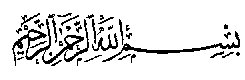
\includegraphics [height=2cm, width=8cm]{konten/gambar/quran.png}
\end{figure}

“Bacalah dengan menyebut nama Tuhanmu
Dia telah menciptakan manusia dari segumpal darah
Bacalah, dan Tuhanmulah yang maha mulia
Yang mengajar manusia dengan pena, Dia mengajarkan manusia apa yang tidak diketahuinya..”

\begin{center}
	\centering (QS. Al-‘Alaq1-5)
\end{center}

\begin{center}
	Alhamdulillah, Alhamdulillah, Alhamdulillahirobbil’alamin. Segala puji bagi Allah SWT, Tuhan yang Maha Agung dan Maha Tinggi.Sujud syukur kupersembahkan kepada-Mu, dengan Rahmat dan Rahim-Mu telah kau jadikan aku manusia yang senantiasa berpikir, berilmu, beriman dan bersabar dalam menjalani kehidupan ini.Semoga keberhasilan ini menjadi satu langkah awal bagiku untuk meraih cita-cita besarku.
\end{center}
\begin{center}
	Dengan lantunan Al-fatihah beriring shalawat serta menadahkan tangan didalam doa, terimakasih kepersembahkan untuk-Mu. Kupersembahkan karya kecil ini sebagai tanda bakti, hormat, dan rasa terimakasih yang tiada terhingga kepada Ibu dan Ayah yang telah memberikan kasih sayang, segala dukungan, dan cinta kasih yang tiada terhingga yang tiada mungkin dapat kubalas hanya dengan selembar kertas yang bertuliskan kata cinta dan persembahan. Semoga ini menjadi langkah awal untuk membuat Ibu dan Ayah bahagia.
\end{center}
\begin{center}
	Ayahanda Agus Zaini dan Ibunda Arnihar  tercinta, terimakasih....
\end{center}
\begin{center}
	Yaa Allah 
\end{center}
\begin{center}
	berikanlah balasan setimpal syurga firdaus untuk mereka dan jauhkanlah mereka dari panasnya sengat hawa apineraka-Mu…
	Amiiiin yaa Rabbal’alamin...Teruntuk Ayah anda dan Ibunda Tercinta..
\end{center}

\begin{center}
	Abdur Rahman
\end{center}

\addChapter{\kataPengantar}
%-----------------------------------------------------------------------------------------------%
%
% Maret 2019
% Template Latex untuk Tugas Akhir Program Studi Sistem informasi ini
% dikembangkan oleh Inggih Permana (inggihjava@gmail.com)
%
% Template ini dikembangkan dari template yang dibuat oleh Andreas Febrian (Fasilkom UI 2003).
%
% Orang yang cerdas adalah orang yang paling banyak mengingat kematian.
%
%-----------------------------------------------------------------------------------------------%

%-----------------------------------------------------------------------------%
\chapter*{\kataPengantar}
%-----------------------------------------------------------------------------%

Assalamu’alaikum warahmatullahi wabarakatuh
Alhamdulillahi Rabbil ‘Alamin, puji syukur penulis ucapkan kehadirat Allah SWT yang telah melimpahkan rahmat dan karunia-Nya sehingga penulis dapat menyelesaiakan Tugas Akhir dengan judul \textbf{“\judulkecil”}. Penulisan Tugas Akhir ini dimaksudkan untuk memenuhi salah satu syarat dalam rangka menyelesaikan studi Strata 1 (S1) di \universitas, shalawat beserta salam selalu tercurahkan kepada Nabi Muhammad SAW, mudah-mudahan kita semua selalu mendapat syafa’at dan dalam lindungan Allah SWT Amin.

Dalam penyusunan dan penyelesaian tugas akhir ini, penulis menyadari bahwa Tugas Akhir ini tidak akan terwujud dengan baik tanpa adanya bantuan dari semua pihak, untuk itu penulis menyampaikan ucapan terima kasih banyak kepada:
\begin{enumerate}
	\item Bapak \rektor, sebagai Rektor \universitas. 
	\item Bapak \dekan, sebagai Dekan \fakultas. 
	\item Ibu \kaprodi, sebagai Ketua Program Studi \programStudi.
	\item Bapak \pembimbingpertama, Selaku dosen pembimbing dalam mengerjakan tugas akhir ini.
	\item Bapak \pengujipertama, Selaku Penguji I (Pertama) dalam mengerjakan tugas akhir ini.
	\item Bapak \pengujikedua, Selaku Penguji II (Kedua) dalam mengerjakan tugas akhir ini.
	
	\item	Ibu Siti Monalisa, S.T, M.Kom, Selaku Pembimbing Akademis yang telah bersedia menjadi orang tua saya selama menuntut ilmu di \universitas
	\item	Segenap Dosen dan Civitas Akademika pada program studi \programStudi, \fakultas, \universitas.
	\item	Keluarga tercinta khususnya kepada kedua orang tua, ayahanda Agus Zaini dan dan ibu Arnihar. Terima kasih atas do’a dan dukungannya secara moral atau pun moril, serta selalu menjadi inspirasi, motivasi hidupku dalam setiap langkahku di kehidupanku ini. Semoga beliau dalam lindungan Allah SWT dimana pun berada, dan penulis memohon do’a semoga pengorbanan beliau mendapat keridhoan dari Allah SWT. Aamiin.
	\item	Sahabat-sahabat Bakti Yoga, Agung Kurniawan, Harika Faizal, Tomi Zul Hidayat, Nofan Widi Yarna, Tofani Joga dan lain seterusnya yang telah banyak membantu penulis dan memberikan motivasi dan dorongan disetiap waktunya sehingga penulis bias seperti sekarang.
	\item	Keluarga besar \programStudi \ angkatan 2013.
	\item	Serta teman-teman yang telah terlibat dalam perjuangan penyelesaian pendidikan strata 1 (S1) ini yang tidak bisa penulis sebutkan satu persatu.
	
\end{enumerate}




\vspace*{0.1cm}

\begin{flushright}
\kota, \tanggalPersetujuan\\
Penulis,\\
\vspace{3cm}
\textbf{\underline{\penulis}\\
NIM. \nim}

\end{flushright}

 
\addChapter{ABSTRAK}
%-----------------------------------------------------------------------------------------------%
%
% Maret 2019
% Template Latex untuk Tugas Akhir Program Studi Sistem informasi ini
% dikembangkan oleh Inggih Permana (inggihjava@gmail.com)
%
% Template ini dikembangkan dari template yang dibuat oleh Andreas Febrian (Fasilkom UI 2003).
%
% Orang yang cerdas adalah orang yang paling banyak mengingat kematian.
%
%-----------------------------------------------------------------------------------------------%

\chapter*{\MakeUppercase{\judul}}

\fontsize{14}{16.8}
\begin{center}
	\vspace{0.3cm}
	\MakeUppercase{\textbf{\penulis}}\\
	\MakeUppercase{\textbf{NIM: \nim}}\\
	\fontsize{12}{14.4}
	\vspace{0.7cm}

	Tanggal Sidang: \tanggalSidang\\
	Periode Wisuda:\ \ \ \ \ \ \ \ \ \ \ \ \ \ \ \ \ \ \ \ \ \ \ \ \ \ \ \ \ \ \ \ \ \ \ \ \ \ 

	\vspace{0.7cm}
	Program Studi \programStudi\\
	\fakultas\\
	\universitas\\
	\alamatUniversitas\\

	\vspace{0.7cm}
\end{center}

\fontsize{12}{14.4}
\begin{center}\MakeUppercase{\textbf{Abstrak}}\end{center}

\noindent
\fontsize{10pt}{12pt}\selectfont
Salah satu hewan yang sering dijadikan kurban pada saat hari raya Idul Adha adalah sapi. Ada banyak kriteria yang harus diperhatikan dalam menentukan kelayakan seekor sapi untuk dijadikan kurban. Kriteria-kriteria tersebut sering diabaikan oleh masyarakat. Hal ini dikarenakan ketidaktahuan masyarakat tentang kriteria-kriteria tersebut. Disamping itu, jumlah pakar yang bisa menilai kelayakan hewan kurban dan mensosialisasikan hal tersebut ke masyarakat sangat terbatas. DST... (Maksimal 200 kata)\\
\noindent{\textbf{Kata Kunci:} \textit{forward chaining}, sapi, DST (Maksimal 5)} \\

\addChapter{\emph{ABSTRACT}}
%-----------------------------------------------------------------------------------------------%
%
% Maret 2019
% Template Latex untuk Tugas Akhir Program Studi Sistem informasi ini
% dikembangkan oleh Inggih Permana (inggihjava@gmail.com)
%
% Template ini dikembangkan dari template yang dibuat oleh Andreas Febrian (Fasilkom UI 2003).
%
% Orang yang cerdas adalah orang yang paling banyak mengingat kematian.
%
%-----------------------------------------------------------------------------------------------%

\chapter*{\MakeUppercase{\textit{\judulInggris}}}

\fontsize{14}{16.8}
\begin{center}
	\vspace{0.3cm}
	\MakeUppercase{\textbf{\penulis}}\\
	\MakeUppercase{\textbf{NIM: \nim}}\\
	\fontsize{12}{14.4}
	\vspace{0.7cm}

	\textit{Date of Final Exam: \tanggalSidangInggris}\\
	\textit{Graduation Period:}\ \ \ \ \ \ \ \ \ \ \ \ \ \ \ \ \ \ \ \ \ \ \ \ \ \ \ \ \ \ \ \ \ \ \ \ \ \ 

	\vspace{0.7cm}
	\emph{Department of \programStudiInggris}\\
	\textit{\fakultasInggris}\\
	\universitasInggris\\
	\alamatUniversitasInggris\\

	\vspace{0.7cm}
\end{center}

\fontsize{12}{14.4}
\begin{center}\MakeUppercase{\textbf{\emph{Abstract}}}\end{center}

\noindent
\fontsize{10pt}{12pt}\selectfont
\emph{}\\
\noindent{\emph{\textbf{Keywords:} DOG, DOG, DST (Maksimal 5)}} \\
	}{}

\fontsize{12pt}{14.4pt}\selectfont

\phantomsection
\tableofcontents
\clearpage
\phantomsection
\listoffigures
\clearpage
\phantomsection
\listoftables
\clearpage

\addChapter{DAFTAR SINGKATAN}
%-----------------------------------------------------------------------------------------------%
%
% Maret 2019
% Template Latex untuk Tugas Akhir Program Studi Sistem informasi ini
% dikembangkan oleh Inggih Permana (inggihjava@gmail.com)
%
% Template ini dikembangkan dari template yang dibuat oleh Andreas Febrian (Fasilkom UI 2003).
%
% Orang yang cerdas adalah orang yang paling banyak mengingat kematian.
%
%-----------------------------------------------------------------------------------------------%

%-----------------------------------------------------------------------------%
\chapter*{DAFTAR SINGKATAN}
%-----------------------------------------------------------------------------%
\begin{tabular}{lll}
DINKES &:& Dinas Kesehatan\\
HTML &:& \textit{Hyper Text Markup Language}\\
PHP &:&\textit{Pear Hypertext Preposessor}\\
PHBS &:& Perilaku Hidup Bersih dan Sehat\\
SDM &:& Sumber Daya Manusia\\
SE &:& Software Engineering\\
SIK &:& Meningkatkan kualitas Sistem Informasi Kesehatan\\
UML &:& \textit{Unifield Modelling Language}\\
\end{tabular}
\renewcommand{\headrulewidth}{0.0pt}
  \fancyhf{} 
  \fancyhead[L]{} 
  \fancyhead[C]{} 
  \fancyhead[R]{}
  \fancyfoot[C]{}
  \fancyfoot[R]{\thepage} 
  \renewcommand{\headrulewidth}{0.0pt}  
  \renewcommand{\footrulewidth}{0.0pt} 
\pagestyle{fancy}

\makeatletter
\renewcommand\chapter{\if@openright\cleardoublepage\else\clearpage\fi
                    \thispagestyle{empty}%
                    \global\@topnum\z@
                    \@afterindentfalse
                    \secdef\@chapter\@schapter}
\makeatother

\fontsize{12pt}{14.4pt}\selectfont

\pagenumbering{arabic}
%-----------------------------------------------------------------------------------------------%
%
% Maret 2019
% Template Latex untuk Tugas Akhir Program Studi Sistem informasi ini
% dikembangkan oleh Inggih Permana (inggihjava@gmail.com)
%
% Template ini dikembangkan dari template yang dibuat oleh Andreas Febrian (Fasilkom UI 2003).
%
% Orang yang cerdas adalah orang yang paling banyak mengingat kematian.
%
%-----------------------------------------------------------------------------------------------%

%-----------------------------------------------------------------------------%
\chapter{\babSatu}
%-----------------------------------------------------------------------------%

%-----------------------------------------------------------------------------%
\section{Latar Belakang}
%-----------------------------------------------------------------------------%
Surat adalah alat atau sarana komunikasi yang baik dalam bentuk tulisan maupun gambar yang digunakan oleh pihak-pihak terkait seperti perusahaan, organisasi, maupun pribadi kepada pihak lain untuk menyampaikan suatu informasi yang berfungsi sebagai bukti konkrit pada suatu hal atau kejadian tertentu \cite{triyono2013pembuatan}. Dalam suatu organisasi/perusahaan surat menurut prosedur pengurusannya dibagi menjadi dua yaitu surat masuk dan surat keluar. Surat masuk merupakan komunikasi tertulis berupa semua jenis surat yang diterima dari perusahaan atau instansi lain kepada pihak penerima. Surat masuk merupakan semua jenis surat yang diterima dari instansi lain maupun perorangan, baik yang diterima melalui pos maupun yang diterima melalui kurir dengan mempergunakan buku pengiriman/ekspedisi, sedangkan surat keluar adalah surat yang sudah lengkap (bertanggal, bernomor, berstempel, dan telah ditanda tangani oleh pejabat yang berwenang) yang dibuat oleh suatu instansi, kantor atau lembaga untuk ditujukan atau dikirim kepada instansi, kantor atau lembaga lain \cite{suherman2017sistem}.

Prosedur pengelolaan surat masuk meliputi; pengelompokan surat, membuka surat, pemerikasaan surat, pencatatan surat dan pendistribusian surat, sedangkan untuk surat keluar meliputi; pembuatan konsep, persetujuan konsep, pengertian surat, pemberian nomor, penyusunan surat, pengiriman surat. Prosedur pengolahan surat perlu diterapkan untuk masing-masing unit organisasi, karena merupakan sumber data atau informasi yang bermanfaat untuk kemajuan organisasi tersebut secara maksimal.

Kegiatan atau pekerjaan kantor yang berhubungan dengan penyimpanan dan pengelolaan warkat, surat surat dan dokumen - dokumen ini disebut kearsipan. Kearsipan memegang peranan penting bagi kelancaran suatu organisasi.

Sebagai salah satu kantor pemerintah yang tidak terlepas dengan kegiatan surat menyurat sebagai sarana komunikasi dengan pihak internal dan eksternal organisasi, penatausahaan surat dan arsip sangat dibutuhkan sebagai kegiatan pendukung bagi pelaksanaan tugas pokok Kantor Dinas Kesehatan Kabupaten Pelalawan (DINKES) yang merupakan instansi di daerah yang berhubungan langsung dengan satuan kerja dibidang advokasi kesehatan. Walaupun bukan merupakan pokok pelayanan organisasi, kegiatan ini menjadi sangat penting disebabkan dapat menjadi salah satu tolok ukur/indicator kinerja DINKES terhadap pemangku kepentingan.

Saat ini, di DINKES terdapat beberapa aplikasi yang dapat digunakan dalam penatausahaan surat dan arsip. Pada pelaksanaannya, penatausahaan surat belum memanfaatkan aplikasi penatausahaan surat dan masih dilakukan secara manual, disisi lain pemanfaatan aplikasi arsip belum digunakan secara menyeluruh di setiap unit kerja di DINKES yang berdampak pada penatausahaan arsip kurang efisien baik arsip fisik maupun arsip elektronik. Selain itu aplikasi yang ada tidak mengakomodasi alur proses yang melibatkan bagian-bagian di DINKES kebutuhan setiap bagian dalam pemantauan penyelesaian surat keluar. Penatausahaan dengan cara manual selama ini memiliki beberapa keterbatasan sebagai berikut :
\begin{enumerate}
\item Manajemen surat kurang efisien disebabkan waktu yang dibutuhkan dalam pencatatan secara manual dan distribusi fisik surat kepada masing-masing unit kerja
\item Terjadi duplikasi data dan fungsi, hal ini disebabkan masing-masing bagian melakukan penatausahaan arsip tersendiri baik arsip elektronik maupun arsip fisik,
\item Kesulitan dalam pencarian surat untuk keperluan referensi disebabkan arsip surat dan data elektronik surat keluar belum dikelola dengan baik.
\item Pengawasan kemajuan penerbitan surat keluar dan penyelesaian surat yang dapat dihubungkan dengan pengawasan kinerja pegawai tidak dapat dilakukan dengan baik.
\end{enumerate}

Pengembangan sistem informasi penatausahaan surat dan arsip untuk instansi DINKES memang telah banyak dilakukan. Tetapi sistem informasi yang dikembangkan tidak memperhatikan proses bisnis yang melibatkan berbagai bagian pada DINKES dan rata-rata bersifat standalone. Oleh karenanya dibutuhkan dibutuhkan pengembangan sistem informasi baru yaitu “\namasistem \ (\singkatansistem)” yang digunakan untuk menatausahakan surat yang mengakomodasi alur proses dan pengawasan kemajuan penerbitan surat dan penyelesaian surat dalam rangka pengawasan kinerja. Sitsar merupakan aplikasi berbasis web yang dikembangkan dengan Bahasa pemrograman PHP dengan pemilihan basis data MySQL. PHP dipilih karena kemudahannya, cepat dan bersifat multiplatform. Sedangkan MySQL merupakan basis Data yang digunakan pada aplikasi-aplikasi DINKES.
Dengan latar belakang di atas, menjadi dasar pertimbangan penulis untuk membuat laporan penelitian tugas akhir ini dengan mengangkat judul \textbf{“\judulkecil.”} 



%-----------------------------------------------------------------------------%
\section{Perumusan Masalah}
%-----------------------------------------------------------------------------%
Rumusan masalah penelitian ini adalah : \rumusanmasalah \ ?


%-----------------------------------------------------------------------------%
\section{Batasan Masalah}
%-----------------------------------------------------------------------------%
Adapun Batasan masalaah yang terdapat dalam penelitian kali ini sebagai berikut:
\begin{enumerate}
	\item Sistem yang dikembangkan adalah untuk mempermudah tatakelola surat dan arsip pada dinas kesehatan kabupaten pelalawan.
	\item Sistem informasi tatakelola surat dan arsip ini hanya membahas tentang surat masuk, surat keluar serta arsip surat.
	\item Sistem informasi tatakelola surat ini dibangun menggunakan Php sebagai Bahasa pemrograman dan Mysql sebagai database.
	\item Pengembangan system menggunakan metode waterfall
	\item Sistem ini menggunakan \textit{Unifield Modelling Language} (UML) sebagai
	toolsnya.
	\item Pengujian Sistem Menggunakan \textit{Black Box} Testing.
\end{enumerate}

%-----------------------------------------------------------------------------%
\section{Tujuan}
%-----------------------------------------------------------------------------%
Adapun tujuan dari penelitian tugas akhir ini adalah:
\begin{enumerate}
	\item Merancang sebuah sistem yang sudah terkomputerisasi untuk mendukung kebutuhan informasi mengenai pengolahan data tatakelola surat dan pengarsipan pada Subbagian Umum dan Kepegawaian pada Dinas Kesehatan Kabupaten Pelalawan.
	\item Menganalisa objek dan data pendukungnya untuk pembuatan sistem informasi arsip dokumen pada Subbagian Umum dan Kepegawaian pada Dinas Kesehatan Kabupaten Pelalawan.
	\item Untuk memudahkan pekerjaan dalam mencari atau penginputan surat dan arsip.
\end{enumerate}

%-----------------------------------------------------------------------------%
\section{Manfaat}
%-----------------------------------------------------------------------------%
Manfaat tugas akhir ini adalah:
\begin{enumerate}
	\item Dapat meminimalisir permasalahan yang terjadi pada Subbagian Umum dan Kepegawaian pada Dinas Kesehatan Kabupaten Pelalawan.
	\item Dapat membantu Subbagian Umum dan Kepegawaian dalam pengendalian tatakelola surat dan pengarsipan surat, baik itu dari segi waktu, tenaga dan juga biaya.
	\item Dapat memudahkan Dinas Kesehatan Kabupaten Pelalawan dalam memprioritaskan surat menurut kepentingan surat tersebut.
\end{enumerate}

%-----------------------------------------------------------------------------%
\section{Sistematika Penulisan}
%-----------------------------------------------------------------------------%
Sistematika penulisan laporan adalah sebagai berikut:

\textbf{BAB 1. \babSatu}

BAB 1 pada tugas akhir ini berisi tentang: (1) latar belakang masalah; (2) rumusan masalah; (3) batasan masalah; (4) tujuan; (5) manfaat; dan (6) sistematika penulisan.

\textbf{BAB 2. \babDua}

BAB 2 pada tugas akhir ini berisi tentang: tentang teori-teori yang berasal dari jurnal, buku serta studi kepustakaan yang digunakan sebagai landasan teori dalam pembuatan tugas akhir ini seperti tentang pengertian sistem informasi, manajemen data dan pengawasan.


\textbf{BAB 3. \babTiga}

BAB 3 pada tugas akhir ini berisi tentang: tentang metodologi atau urutan tata cara dan langkah-langkah penelitian dari tahap persiapan sampai dengan tahap mengembangkan sistem pengawasan.


\textbf{BAB 4. \babEmpat}

BAB 4 pada tugas akhir ini berisi tentang: penjelaskan tentang uraian permasalahan, analisis permasalahan dan perancangan sistem tahap dimana akan dibuat flowchart Alur Sistem Informasi menggunakan tool – tool UML (United Modelling Languange). Diagram-diagram yang digunakan dalam UML (United Modelling Languange) : usecase, sequence, class, activity.

\textbf{BAB 5. \babLima}

BAB 5 pada tugas akhir ini berisi tentang: penjelasan mengenai batasan implementasi, lingkungan implementasi dan hasil dari implementasi. Serta menjelaskan pengujian perangkat lunak dan hasil pengujian.

\textbf{BAB 6. \babEnam}

BAB 6 pada tugas akhir ini berisi tentang: tentang kesimpulan dan saran dari penelitian Tugas Akhir.
%-----------------------------------------------------------------------------------------------%
%
% Maret 2019
% Template Latex untuk Tugas Akhir Program Studi Sistem informasi ini
% dikembangkan oleh Inggih Permana (inggihjava@gmail.com)
%
% Template ini dikembangkan dari template yang dibuat oleh Andreas Febrian (Fasilkom UI 2003).
%
% Orang yang cerdas adalah orang yang paling banyak mengingat kematian.
%
%-----------------------------------------------------------------------------------------------%

%-----------------------------------------------------------------------------%
\chapter{\babDua}
%-----------------------------------------------------------------------------%

%-----------------------------------------------------------------------------%
%\section{Penelitian Terdahulu}
%-----------------------------------------------------------------------------%
%-----------------------------------------------------------------------------%
\section{Sistem Informasi}
%-----------------------------------------------------------------------------%
Menurut \citeA{suherman2017sistem} Sistem informasi adalah kerangka kerja yang mengkoordinasikan sumber daya (manusia, komputer) untuk mengubah masukan (input) menjadi sebuah keluaran (informasi), guna mencapai sasaran-sasaran perusahaan . Sistem Informasi adalah bagian dari empat bagian utama. Keempat bagian utama nya mencakup perangkat lunak (software), perangkat keras (hardware), infrastruktur dan Sumber Daya Manusia (SDM) yang terlatih. Keempat bagian utama ini saling berkaitan untuk menciptakan sebuah sistem yang dapat mengolah data menjadi informasi yang bermanfaat (Pratama, 2014).


%-----------------------------------------------------------------------------%
\section{Pengertian Arsip}
%-----------------------------------------------------------------------------%
Menurut Undang-Undang Nomor 43 Tahun 2009 Tentang Kearsipan, arsip merupakan rekaman kegiatan atau peristiwa dalam berbagai bentuk dan media sesuai dengan perkembangan teknologi informasi dan komunikasi yang dibuat dan diterima oleh lembaga negara, pemerintah daerah, lembaga pendidikan, perusahaan, organisasi politik, organisasi kemasyarakatan, dan perseorangan dalam pelaksanaan kehidupan bermasyarakat, berbangsa, dan  bernegara. Menurut The Liang Gie, arsip merupakan sekumpulan warkat dalam corak apapun baik dalam bentuk tunggal maupun kelompok yang disimpan secara sistematis dan apabila diperlukan dapat diketemukan kembali dengan mudah, cepat, dan tepat (Iin Kristiyanti, 2015). Menurut Kamus Besar Bahasa Indonesia (Hasan Alwi, 2003), arsip merupakan simpanan surat-surat penting. Sebuah surat dapat dinyatakan sebagai arsip jika memenuhi persyaratan sebagai berikut:
\begin{enumerate}
	\item Surat tersebut harus masih mempunyai kepentingan bagi organisasi/lembaga baik untuk masa sekarang maupun masa yang akan datang.
	\item Surat yang masih mempunyai kepentingan tersebut disimpan menurut sistem tertentu sehingga memudahkan dalam penemuan kembali ketika diperlukan.
	
\end{enumerate}


%-----------------------------------------------------------------------------%
\section{Model Pengembangan Sistem}
%-----------------------------------------------------------------------------%
Dalam penelitian ini, model pengembangan sistem yang digunakan adalah waterfall. Menurut Pressman dalam Itqan (2018) Model Waterfall adalah model klasik yang bersifat sistematis, berurutan dalam membangun software. Nama model ini sebenarnya adalah “\textit{Linear Sequential Model}”. Model ini sering disebut juga dengan “\textit{classic life cycle}” atau metode waterfall. Model ini termasuk model generic pada rekayasa perangkat lunak dan pertama kali di perkenalkan oleh Winston Royce sekitar tahun 1970 sehingga sering dianggap kuno, tetapi merupakan model yang paling banyak di pakai dalam \textit{Software Engineering} (SE). disebut dengan \textit{waterfall} karena tahap demi tahap yang dilalui harus menunggu selesainya tahap sebelumnya dan berjalan berurutan.
Model pengembangan sederhana ditunjukkan pada \pic~\ref{gbr201}. Ini dikenal secara tradisional sebagai model air terjun.

\begin{figure}
	\centering
	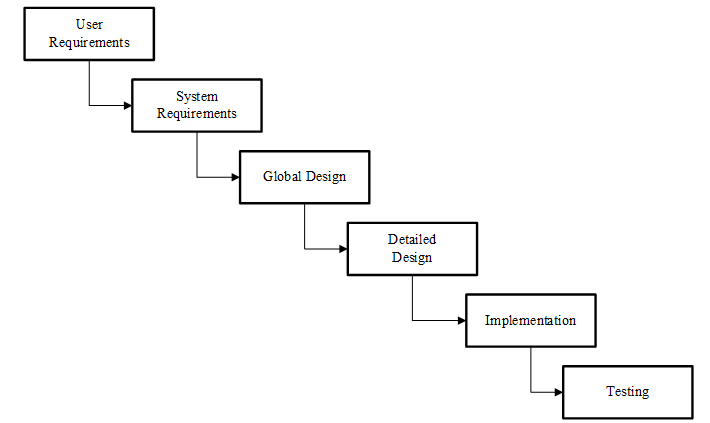
\includegraphics [height=8cm, width=13cm]{konten/gambar/gbr201.png}
	\caption{Metode Waterfall}
	\label{gbr201}
\end{figure}
%-----------------------------------------------------------------------------%
\section{Perancangan Sistem}
%-----------------------------------------------------------------------------%
Perancangan sistem adalah proses pembuatan rancangan suatu sistem berdasarkan hasil dari tahap analisis sistem. Dalam proses perancangan sistem memuat berbagai uraian mengenai input, proses, dan output dari sistem yang diusulkan (Setiawan, 2013).
Perancangan sistem bertujuan untuk memberikan gambaran apa yang seharusnya di kerjakan bagaimana tampilannya (Damayanti \& Sulistiani, 2017).
Perancangan sistem merupakan tahap selanjutnya setelah analisa sistem, mendapatkan gambaran dengan jelas tentang apa yang dikerjakan pada analisa sistem, maka dilanjutkan dengan memikirkan bagaimana membentuk sistem tersebut.Tujuan Perancangan Sistem (Kristanto, 2008):

\begin{enumerate}
	
	\item Untuk memenuhi kebutuhan pemakaian sistem (\textit{user}).
	\item Untuk memberikan gambaran yang jelas dan menghasilkan rancangan bangun yang lengkap kepada pemograman komputer dan ahli-ahli teknik lainnya yang terlibat dalam pengembangan atau pembuatan sistem
	
\end{enumerate}

%-----------------------------------------------------------------------------%
\section{Tahap Perancangan Sistem}
%-----------------------------------------------------------------------------%
Tahap perencanaan (\textit{planning}) adalah menyangkut studi tentang kebutuhan pengguna (\textit{user specification}), studi-studi kelayakan (\textit{feasibility study}) baik secara teknis maupun secara teknologi serta penjadwalan pengembangan suatu proyek sistem informasi atau perangkat lunak.

\subsection{ Analisis}
Langkah ini merupakan analisa terhadap kebutuhan sistem. Pengumpulan data dalam tahap ini bisa melakukan sebuah penelitian, wawancara atau studi literatur. Sistem analis akan menggali informasi sebanyak-banyaknya daripengguna (\textit{user}) sehingga akan tercipta sebuah sistem komputer yang bisa melakukan tugas-tugas yang diinginkan oleh pengguna (\textit{user}) tersebut. Tahapan ini akan menghasilkan dokumen (\textit{user requirtment} atau bisa dikatakan sebagai data yang berhubungan dengan keinginan (\textit{user} dalam pembuatan sistem. Dokumen ini lah yang akan menjadi acuan sistem analis untuk menerjemahkan ke dalam bahasa pemrogram.
\subsection{ Perancangan Interface}
Tahapan dimana dilakukan penuangan pikiran dan perancangan sistem terhadap solusi dari permasalahan yang ada dengan menggunakan perangkat pemodelan sistem seperti UML diantara seperti \textit{class diagram, use case diagram, activity diagram dan sequence diagram}.
\subsection{ Implementasi}
Tahap implementasi adalah adalah tahap dimana kita mengimplementasikan perancanagan sistem ke situasi nyata, disini kita akan berurusan dengan pemilihan perangkat keras dan penyusunan perangkat lunak.

\subsection{ Pengujian}
Tahap pengujian adalah tahap dimana sistem yang baru diuji kemampuan dan keefektifannya sehingga didapatkan kekurangan dan kelemahan sistem yang kemudian dilakukan pengkajian ulang dan perbaikan terhadap aplikasi menjadi lebih baik dan sempurna.
\subsection{ Pemeliharaan}
Perangkat lunak yang sudah disampaikan kepada pelanggan pasti akan mengalami perubahan. Perubahan tersebut bisa karena mengalami kesalahan karena perangkat lunak harus menyesuaikan dengan lingkungan baru, atau karena pelanggan membutuhkan perkembangan fungsional.
%-----------------------------------------------------------------------------%


%-----------------------------------------------------------------------------%
\section{Website}
%-----------------------------------------------------------------------------%
Menurut Kirana dalam Taufik (2017) menyatakan bahwa website atau situs merupakan tempat penyimpanan data dan informasi dengan menggunakan topik tertentu. Di umpamakan situs web ini adalah sebuah buku yang berisikan sebuah topik tertentu, website atau situs web juga merupakan kumpulan dari halaman- halaman web yang saling berkaitan di dalam web tersebut.
Menurut Anisya dan Yunita (2017) Web adalah sebuah penyebaran informasi melalui internet. Web merupakan hal yang tidak dapat di pisahkan dari dunia internet. Melalui web, setiap pemakai internet bisa mengakses informasi-informasi di situs web yang tidak hanya berupa teks, tetapi juga dapat berupa gambar, suara, film, animasi, dan lain-lain.
Secara umum ada beberapa bahasa pemograman yang di gunakan untuk membuat aplikasi website. Adapun bahasa program yang di pakai sebagai berikut:

\begin{enumerate}
	\item HTML \textit{ (Hyper Text Markup Language)}.
	\item PHP \textit{ (Pear Hypertext Preposessor)}.
	\item CSS \textit{ (Cascading Style Sheet)}.
	\item Javascript.
	\item Mysql.
	\item Jquery.

\end{enumerate}

\subsection{HTML}

HTML \textit{(Hyper Text Markup Language)} adalah sebuah bahasa markup yang digunakan untuk membuat halaman web dan menampilkan berbagai informasi di dalam sebuah browser internet (Anisya dan Yunita, 2017).
HTML \textit{(Hyper Text Markup Language)} merupakan bahsaa yang digunakan untuk mendeskripsikan struktur sebuah halaman web. HTML berfungsi untuk mempublikasikan dokumen online. Statement dasar dari HTML disebut tags. Sebuah tag dinyatakan dalam sebuah kurung siku. Tags yang ditujukan untuk sebuah dokumen atau bagian dari suatu dokumen haruslah dibuat berupa pasangan. Terdiri dari tag penutup menggunakan tambahan tanda garis miring (/) di awal nama tag.(Henderson dalam Omar dkk, 2018)

\subsection{Wampp}
%-----------------------------------------------------------------------------%
WAMPP merupakan salah satu paket \textit{installasi Apache, PHP dan MySQL}instant yang dapat kita gunakan untuk membantu proses installasi ketiga produk tersebut. Selain paket installasi instant WAMPP versi 3.2 juga memberikan fasiltias pilihan pengunaan PHP5 atau PHP7. Untuk berpindah versi PHP yang ingin digunakan juga sangat mudah dilakukan dengan mengunakan bantuan \textit{PHP Switch} yang telah disertakan oleh WAMP dan yang terpenting WAMP bersifat \textit{free} atau gratis untuk digunakan.
Sejarah singkat WAMP, WAMP merupakan pengembangan dari LAMP
\textit{(Linux Apache, MySQL, PHP and PERL)}, WAMP ini merupakan \textit{project} nonprofit yang di kembangkan oleh \textit{Apache Friends} yang didirikan Kai 'Oswalad'Seidler dan Kay Vogelgesang pada tahun 2002, \textit{project} mereka ini bertujuan mempromosikan pengunaan \textit{Apache} web server.

\subsection{PHP}
PHP \textit{(Pear Hypertext Preposessor)} merupakan sebuah bahasa Scripting yang di bundle dengan HTML yang di jalankan disisi \textit{Server}. Sebagian besar perintahnya berasal dari bahasa C, Java dan Perl dengan beberapa tambahan fungsi PHP (Anisya dan Yunita, 2017). Sedangkan, menurut Abdul dan Kasmawi (2016) PHP adalah salah satu skrip bahasa pemograman yang di rancang untuk membangun aplikasi \textit{web}. PHP dibangun dalam bentuk skrip yang di tempatkan dan di proses \textit{server}. Hasilnya akan dikirimkan ke \textit{client}, tempat pemakai menggunakan \textit{browser}. Secara khusus, PHP dirancang untuk membentuk web dinamis. Artinya, ia dapat membentuk suatu tampilan berdasarkan permintaan terkini, misalnya dapat menampilkan isi basis data ke halaman web.


\subsection{MySQL}
MySQL merupakan bahasa standar yang digunakan untuk memanipulasi data dan memperoleh data dari sebuah database relasional. SQL merupakan bahsa standar yang digunakan untuk memanipulasi data dan memperoleh data dari database relasional. SQL memungkinkan seorang pengguna untuk mengakses informasi tanpa mengetahui bagaimana informasi tersebut disusun. SQL dilengkapi dengan sejumlah perintah untuk melakukan manipulasi data. (Anisya dan Yunita, 2016)
MySQL adalah salah satu jenis \textit{database server} yang menggunakan SQL \textit{(Structured Query Language)} sebagai bahasa dasar untuk mengakses \textit{database-nya}. MySQL termasuk jenis \textit{Relational Database Management System}(RDBMS), sehingga istilah seperti tabel, baris dan kolom digunakan pada MySQL. MySQL sangat populer dikalangan pengembang perangkat lunak karena MySQL merupakan \textit{database server} yang gratis dan cepat. Selain itu, dukungan dari perusahaan dan komunitas yang memadai membuat MySQL menjadi \textit{database server} yang disukai dan termasuk dalam kategori database yang handal.(Arifudzaki dalam abdul dan kasmawi, 2016).

%-----------------------------------------------------------------------------%
\section{Dinas Kesehatan Kabupaten Pelalawan}
%-----------------------------------------------------------------------------%
\subsection{Visi dan Misi Instansi}

Mewujudkan Pelayanan Kesehatan Berkualitas dan Berkeadilan Menuju Masyarakat Pelalawan Sehat Untuk mencapai visi yang telah ditetapkan, maka ditetapkan misi Dinas Kesehatan sebagai berikut :
\begin{enumerate}
	
	\item Meningkatkan dan memantapkan manajemen dan kinerja serta pelayanan kesehatan yang terjangkau, bermutu, adil dan merata di semua tingkat administrasi dan unit-unit pelayanan kesehatan.
	
	\item Meingkatkan dan mengembangkan promosi kesehatan dan membudayakan Perilaku Hidup Bersih dan Sehat (PHBS) di masyarakat.
	
	\item Meningkatkan kinerja dan memperkuat 
	upaya-upaya pengendalian penyakit dan mewujudkan lingkungan
	sehat, serta penanggulan masalah gizi masyarakat.
	
	\item Meningkatkan kualitas Sistem Informasi Kesehatan (SIK).
	
	\item Memantapkan kemitraan lintas sektor dan pemberdayaan masyarakat.
\end{enumerate}

\subsection{Struktur Organisasi Instansi}
%-----------------------------------------------------------------------------%
Struktur organisasi pada dinas kesehatan kabupaten pelalawan dapat dilihat pada \pic~\ref{StrukturOrganisasi}

\begin{figure}
	\centering
	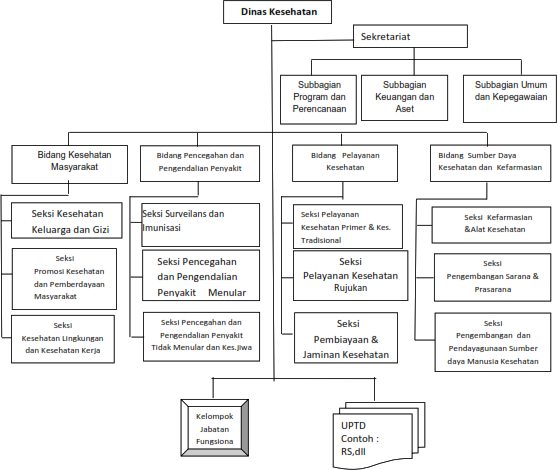
\includegraphics [height=13cm, width=13cm]{konten/gambar/StrukturOrganisasi.png}
	\caption{Struktur Organisasi}
	\label{StrukturOrganisasi}
\end{figure}


%-----------------------------------------------------------------------------------------------%
%
% Maret 2019
% Template Latex untuk Tugas Akhir Program Studi Sistem informasi ini
% dikembangkan oleh Inggih Permana (inggihjava@gmail.com)
%
% Template ini dikembangkan dari template yang dibuat oleh Andreas Febrian (Fasilkom UI 2003).
%
% Orang yang cerdas adalah orang yang paling banyak mengingat kematian.
%
%-----------------------------------------------------------------------------------------------%


%-----------------------------------------------------------------------------%
\chapter{\babTiga}
%-----------------------------------------------------------------------------%


%-----------------------------------------------------------------------------%
\section{Metode Pengembangan Sistem}

Pada metode ini akan membahas tetang metodologi penelitian yang dilakukan dalam penyusunan Tugas Akhir ini menggunakan metode \textit{Waterfall} meliputi \textit{User Requitmetns, System Requitments Analisis, Design}, Impelentasi, Sistem adapun dalam penelitian ini penulis membatasi tahapan penelitian hingga tahapan Implementasi sedangkan tahapan Sistem digantikan dengan tahapan Dokumentasi Laporan Tugas Akhir dapat dilihat pada \pic~\ref{gbr301}.


\begin{figure}
	\centering
	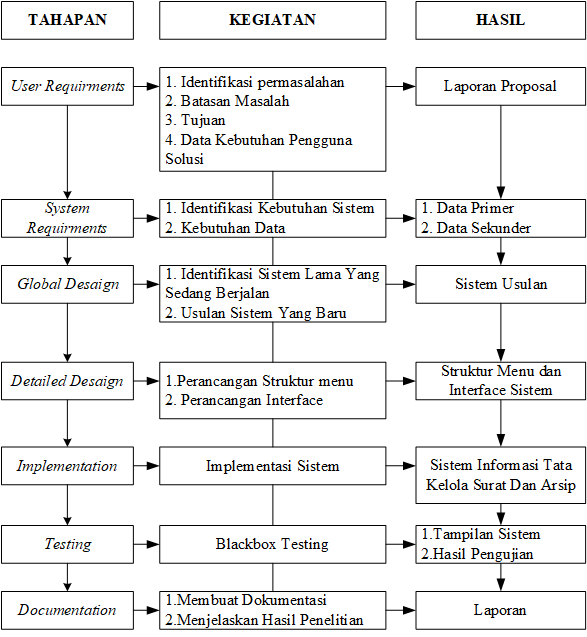
\includegraphics [height=8cm, width=10cm]{konten/gambar/gbr301.png}
		\caption{Metodologi Penelitian}
	\label{gbr301}
\end{figure}

\subsection{\textit{User Requitments}}
Tahap kebutuhan user merupakan tahap mengidentifikasi siapa saja user yang memiliki akses dan tugas masing-masing. Hal ini sangat penting karena kebutuhan pengguna atau user yang terlibat akan menggunakan sistem.

\subsection{\textit{System Requitments}}
Identifikasi Kebutuhan Sistem
Dalam analisa kenbutuhan sistem ada hal-hal yang di perhatikan untuk mengidentifikasi untuk perancangan sistem kedepannya. Hal-hal yang dilakukan pada tahap ini adalah :
Mengidentifikasi masalah alur sistem yang sedang berjalan Dinas Kesehatan Kabupaten Pelalawan dan penulis mewawancarai Kepala Bagian Umum Dinas Kesehatan Kabupaten Pelalawan. Pengambilan data yang dihasilkan dalam wawancara baik berupa data wawancara dan keterangan serta pernyataan narasumber.
\begin{enumerate}
	\item 	Data Primer
	\begin{enumerate}
		\item 	Observasi \\
		Pada tahap observasi ini untuk mengumpulkan informasi tentang lebih mengetahui permasalahan yang diteliti dan kondisi di lapangan (system requirements). Observasi dalam penelitian ini bertujuan untuk memperoleh gambaran mengenai objek penelitian di Dinas Dinas Kesehatan Kabupaten Pelalawan dengan pengambilan data yang dibutuhkan.
		\item 	Dokumen Surat\\
		Pengambilan data serta informasi tata naskah dinas pada Dinas Kesehatan Kabupaten Pelalawan.
		\item	Studi Pustaka\\
		Untuk menambah referensi, penulis melakukan studi pustaka dengan mencari referensi yang terkait dengan topik penelitian tugas akhir ini. Sumber yang penulis gunakan adalah buku-buku dan jurnal yang berkaitan dengan topik penelitian serta data sekunder yang didapat dari Dinas Kesehatan Kabupaten Pelalawan.
	\end{enumerate}
	
	\item Data Sekunder \\
	Data sekunder yaitu data yang diperoleh secara tidak langsung atau data yang diperoleh selain dari objek penelitian. Dalam penelitian ini sumber data sekunder yang digunakan berbentuk data file baik foto dan ddokumen yang di dapat langsung dari Dinas Kesehatan Kabupaten Pelalawan dapat dilihat pada Lampiran A 

\end{enumerate}


\subsection{Global Design}
Pada tahap ini merupakan melakukan perancangan sistem yang di usulkan. Tahap Global Design merupakan tahap dalam perancangan sistem yang akan dibangun berdasarkan analisis sistem yang sebelumnya telah dilaksanakan.
\begin{enumerate}
	\item 	Alur Sistem Lama.\\
	Mengetahui alur sistem yang sedang berjalan sebelumnya adalah sebuah langka untuk merancangan sistem usulan yang akan di buat oleh peneliti. Analisis sistem yang sedang berjalan meruapakan analasis sistem yang dilakukan yaitu menganalisa sistem yang saat ini berjalan pada Dinas Kesehatan Kabupaten Pelalawan untuk mengidentifikasi permasalahan-permasalahan yang muncul.
	\item	Perancangan Sistem Usulan\\
	Perancangan sistem usulan adalah sebuah perancangan yang di rancang untuk mengtasi atau meminimalisir permasalahan yang ada pada sistem sebelumnya, adapun langkahnya, yaitu:
	\begin{enumerate}
		\item	Analisa Sistem Usulan\\
		Menganalisa permasalahan yang telah diidentifikasi untuk kemudian digunakan dalam dasar perancangan sistem sebagai solusi dari masalah dan memberikan rekomendasi manfaat sesuai kebutuhan dari instansi terkait. Perancangan alur yang akan dibangun dalam membangun system informasi pariwisataDinas Kesehatan Kabupaten Pelalawan adalah merancang bagaimana alur atau jalannya sistem yang akan dibangun berdasarkan wawancara terhadap pihakDinas Kesehatan Kabupaten Pelalawan dan peranan aktor yang terlibat dalam proses sistem. Perancangan alur sistem yang akan dibangun dirangkum dan di jelaskan pada BAB IV “Analisa dan Perancangan”.
		\item	Identifikasi Kebutuhan Sistem\\
		Tahapan ini berguna untuk mengidentifikasi dan menentukan kebutuan sistem yang akan di usulkan.
	\end{enumerate}
\end{enumerate}

\subsection{\textit{Design Detailed}}
Pada tahap ini perancangan yang di jelaskan lebih spesifik tetang perancangan sistem, adapun perancangannya, yaitu:
\begin{enumerate}
	\item 	Perancangan Struktur Menu\\
	Pada perancangan struktur menu terdapat  menu pada sistem yang akan dibangun. Perancangan struktur menu dibuat berdasarkan alur sistem yang telah dibangun sebelumnya. Struktur menu yang akan dirancang dibuat menggunakan tool Microsoft Visio 2019 yang dirangkum dalam BAB IV “Analisa dan Perancangan”.
	\item	Perancangan Interface\\
	Perancangan interface sistem bagaimana tampilan dari sistem yang akan dibangun peneliti. Interface tersebut didesain berdasarkan alur serta struktur menu yang telah dirancang sebelumnya. Interface sistem ini dibuat menggunakan tool Mockups Balsamic 3 yang terangkum dalam BAB IV “Analisa dan Perancangan”.
	\item	Perancangan sistem menggunakan UML dengan 4 (empat) Diagram yaitu, \textit{Use Case Diagram, Sequence Diagram, Class Diagram dan Activity Diagram}.
\end{enumerate}

\subsection{\textit{Implementation}}
Tahap Implementasi merupakan bagian pembuatan kode-kode program yang dibuat berdasarkan seluruh rancangan yang telah dibuat sebelumnya untuk proses selanjutnya, pengolahan data dan pembuatan sistem informasi tatakelola surat dan arsip. Kegiatan dari tahap implementasi meliputi:
\begin{enumerate}
	\item 	Pengolahan Data\\
	Pengolahan data spasial menggunakan database MySQL, dengan server Apache Server, framework Codeigniter dan bootsraap sebagai tampilan interface.
	\item 	Pembuatan kode-kode program atau coding menggunakan Bahasa pemograman PHP.
	\item 	Pada tahap pengkodingan ini dilakukan setelah data yang dibutuhkan terkumpul dan telah diolah sesuai kebutuhan untuk merancang sistem informasi tatakelola surat dan arsip di Dinas kesehatan Kabupaten pelalawan.
\end{enumerate}

\subsection{\textit{Testing}}
Tahap pengujian adalah  tahap yang dilakukan adalah melakukan pengujian menggunakan Blackbox testing yang merupakan pendekatan pengujian dengan mempelajari input dan output yang diberikan.Tahapan pengujian ini di lakukan dengan tujuan untuk menjamin sistem yang dibuat sesuai dengan hasil analisis dan perancangan serta menghasilkan satu kesimpulan apakah sistem tersebut sesuai dengan yang di harapkan.

\subsection{\textit{Documentation}}
Pada tahap ini yang dilakukan adalah melakukan dokumentasi dari semua tahap yang telah dilakukan. Mulai dari proses pendahuluan, perencanaan, pengumpulan data, analisis dan perancangan sistem, implementasi serta pengujian sistem. Kemudian mempresentasikan hasil penelitian dan menampilkan hasil sistem yang telah dibangun. Hasil dari dokumentasi ini adalah laporan Tugas Akhir.


\ifthenelse{\equal{\bidangta}{DUA}}{
  \renewcommand{\babEmpat}{ANALISIS DAN HASIL}
  \renewcommand{\babLima}{PENUTUP}  
}{}

\ifthenelse{\equal{\tipeta}{PROPOSAL TUGAS AKHIR}}{
  \renewcommand{\babEmpat}{JANGKAAN HASIL}
}{}

%-----------------------------------------------------------------------------------------------%
%
% Maret 2019
% Template Latex untuk Tugas Akhir Program Studi Sistem informasi ini
% dikembangkan oleh Inggih Permana (inggihjava@gmail.com)
%
% Template ini dikembangkan dari template yang dibuat oleh Andreas Febrian (Fasilkom UI 2003).
%
% Orang yang cerdas adalah orang yang paling banyak mengingat kematian.
%
%-----------------------------------------------------------------------------------------------%


%-----------------------------------------------------------------------------%
\chapter{\babEmpat}
%-----------------------------------------------------------------------------%
%-----------------------------------------------------------------------------%
\section{Analisa Dan Perancangan Sistem }
%-----------------------------------------------------------------------------%
\subsection{Analisa Sistem terdahulu}
Proses pendokumentasian surat masuk dan keluar pada subbagian umum dan kepegawaian Dinas kesehatan kabupaten pelalawan pada sebuah buku besar. Setiap surat masuk akan dicatat pada subbagian umum dan kepegawaian. Setelah dilakukan pencatatan an pemberian nomer surat masuk, selanjutnya surat tersebut akan didisposisikan pada sub bagian lain atau ke bidang bidang yang dituju oleh si pengirim surat.
Pada surat keluar, setiap surat yang dikeluarkan oleh subbagian dan bidang akan langsung dikirimkan ke tujuan tanpa melewati proses pemberian nomer di subbagian umum dan kepegawaian.


\subsection{Analisa Sistem Usulan}

%-----------------------------------------------------------------------------%


Berdasarkan komunikasi yang dilakukan dengan Kasubag Umum dan kepegawaian, dapat disimpulkan bahwa Dinas Kesehatan(DINKES) membutuhkan sebuah sistem informasi yang dapat membantu proses pengarsipan dokumen dengan spesifikasi sebagai berikut:
\begin{enumerate}
	\item Sistem informasi pengarsipan dikembangan dengan berbasis web.
	\item Sistem dapat diakses oleh 4 (Empat) Aktor, yaitu admin, Kepala Dinas,Pengagenda dan Pegawai.
	\item Sistem dilengkapi dengan login untuk masuk ke dalam sistem informasi.
	\item Sistem dapat melakukan pengelolaan surat masuk maupun keluar, meliputi tambah data, memperbarui data, menampilkan surat dan menghapus surat
	\item Sistem dapat melakukan upload file dalam  menambahkan data surat.
	\item Sistem dapat melakukan pengelolaan pegawai, meliputi tambah pegawai, memperbarui data pegawai, melihat data pegawai, dan menghapus data pegawai.
\end{enumerate}

\section{Perancangan \textit{Unifield Modelling Language} (UML)}
%-----------------------------------------------------------------------------%
\subsection{Skenario Use Case}
\begin{enumerate}
	\item	Halaman \textit{Use Case Diagram} sistem usulan\\
	\textit{Use Case Diagram} dapat dilihat pada \pic~\ref{UseCaseSistemUsulan}.
	\begin{figure}
		\centering
		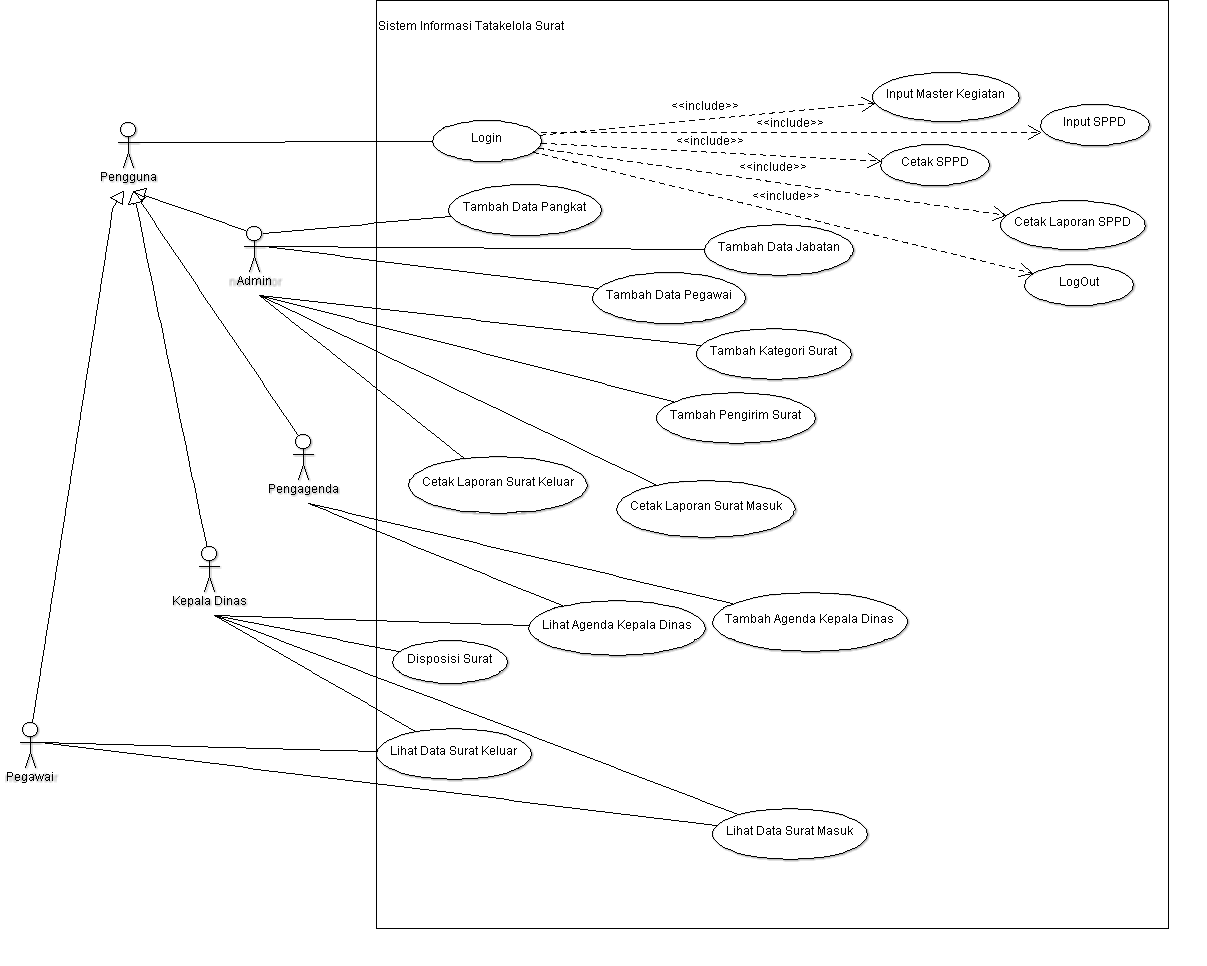
\includegraphics [height=8cm, width=10cm]{konten/gambar/UML/UseCaseDiagram2.png}
		\caption{Use Case Sistem Usulan}
		\label{UseCaseSistemUsulan}
	\end{figure}
	
	\item Kebutuhan Pengguna Sistem\\
	adapun Kebutuhan Pengguna sistem dapat dilihat pada \pic~\ref{AktorSistemSurat}.
		\begin{figure}
		\centering
		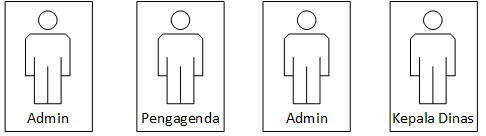
\includegraphics [height=3cm, width=4cm]{konten/gambar/AktorSistemSurat.png}
		\caption{Aktor Sistem Surat}
		\label{AktorSistemSurat}
		\end{figure}
	
	berikut adalah tabel deskripsi tugas dari masing - masing aktor pada \tab~\ref{Useraktor}
	{\fontsize{10pt}{12pt}\selectfont
		\renewcommand\namaTabel{Deskripsi pengguna \textit{user} }
		\begin{longtable}{p{1cm} p{2cm} p{10cm}}
			\caption{\namaTabel}\\
			\label{Useraktor}\\
			\hline
			No. & User & Deskripsi \\ \hline
			\endfirsthead
			%
			\multicolumn{3}{c}%
			{{\bfseries Table \thetable\ Tabel lanjutan ...}} \\
			\hline
			No. & User & Deskripsi \\ \hline
			\endhead
			%
			1. & Admin &  Mengurus \textit{Backend} dari aplikasi  \\
			2. & Pengagenda &  Menginput Data Surat Masuk dan Keluar. \\
			3. & Pegawai & Menerima Surat Masuk dan Keluar \\ 
			4. & Kepala Dinas & Menyetujui dan Mendisposisi Surat Divisi Lain \\ \hline
			%--------------------------------------------------------------------%
			
	\end{longtable}}

	\item Kebutuhan data dalam dalam pengembangan sistem antara lain :
	\begin{enumerate}
		\item data surat
		data surat yang diperlukan antara lain :
		nomer agenda, kategori surat, nomer surat, pengirim surat , perihal surat, isi ringkas dan keterangan surat.
		
		\item data pengguna
		sedangkan data pengguna yang dibutuhkan adalah sebagai berikut :
		nip, nama, golongan, jabatan, alamat dan email.
	\end{enumerate}

	\item Analisa Fitur dan Konten
	
	Adapun fitur dan konten yang terdapat pada aplikasi ini adalah:
	\begin{enumerate}
		\item mengelola data user
		fitur ini dibuat untuk admin yang dapat digunakan untuk menambahkan data user, menghapus data user dan mengesedit data user.
		\item menamhakan data surat
		fitur ini dibuat untuk pengagenda untuk menambahkan data surat masuk dan keluar
		\item menu disposisi
		menu ini dibuat untuk digunakan oleh kepala dinas dan pegawai agar bisa mendisposisikan surat ditingkat instansi.
		\item menu laporan
		menu ini dibuat untuk seluruh pengguna agar bisa mencetak laporan surat masuk dan keluar yang dibutuhkan.
		\item menu SPPD
		menu ini dibuat untuk kepala dinas dan pegawai agar dapat menerbitkan surat perintah perjalanan dinas ditingkat instansi.
	\end{enumerate}
\end{enumerate}

\section{\textit{Class Diagram}}

berikut merupakan desaign dari \textit{class diagram} yang diusulkan dalam sistem tatakelola surat

\section{Perancangan \textit{Database}}

Perancangan \textit{database} digunakan agar  setiap \textit{field} data  yang  mempunyai relasi dapat saling terhubung pada tabel \textit{database}. Perancangan tabel database pada sistem informasi tatakelola surat ini terdiri dari :

\begin{enumerate}
	\item tabel tb\_pegawai
	
	Nama \textit{Database} : Sistasur
	
	Nama tabel : tb\_pegawai
	
	\textit{Field} Kunci : id\_user
	
	Rancangan tabel tb\_pegawai dapat dilihat pada \tab~\ref{tb_pegawai}
	
	{\fontsize{10pt}{12pt}\selectfont
		\begin{longtable}{p{4cm}p{4cm}p{4cm}}
			\caption{Perancangan tabel pegawai}
			\label{tb_pegawai}\\
			\hline
			\textbf{Nama \textit{Field}} & \textbf{\textit{Type Data}} & \textbf{Panjang Data} \\ \hline
			\endfirsthead
			%
			\multicolumn{3}{c}%
			{{\bfseries Table \thetable\ continued from previous page}} \\
			\hline
			\textbf{Nama Field} & Type Data & Panjang Data \\ \hline
			\endhead
			%
			\textit{id\_user}             & \textit{int}       & 8            \\
			nip                 & \textit{varchar}   & 30           \\
			nama\_lengkap        & \textit{varchar}   & 60           \\
			golongan            & \textit{int}       & 8            \\
			jabatan             & \textit{int}       & 8            \\
			alamat              & \textit{text}      & -            \\
			no\_telp             & \textit{varchar}   & 15           \\
			\textit{email}               & \textit{varchar}   & 50           \\
			\textit{username}            & \textit{varchar}   & 40           \\
			\textit{password}            & \textit{varchar}   & 40           \\
			level\_user          & \textit{int}       & 1    \\\hline       
	\end{longtable}}
	
	
	
	
	\item tabel tb\_golongan
	
	Nama \textit{Database} : Sistasur
	
	Nama tabel : tb\_golongan
	
	\textit{Field} Kunci : id\_golongan
	
	Rancangan tabel tb\_pegawai dapat dilihat pada \tab~\ref{tb_golongan}
		
	{\fontsize{10pt}{12pt}\selectfont
		\begin{longtable}{p{4cm}p{4cm}p{4cm}}
			\caption{tabel golongan}
			\label{tb_golongan}\\
			\hline
			\textbf{Nama \textit{Field}} & \textbf{\textit{Type Data}} & \textbf{Panjang Data} \\ \hline
			\endfirsthead
			%
			\multicolumn{3}{c}%
			{{\bfseries Table \thetable\ continued from previous page}} \\
			\hline
			\textbf{Nama Field} & Type Data & Panjang Data \\ \hline
			\endhead
			%
			id\_golongan             & \textit{int}       & 8            \\
			kode\_golongan                 & \textit{varchar}   & 15           \\
			nama\_golongan        & \textit{varchar}   & 50           \\
			alamat              & \textit{text}      & -            \\\hline
	\end{longtable}}


	\item tabel tb\_jabatan
	
	Nama \textit{Database} : Sistasur
	
	Nama tabel : tb\_jabatan
	
	\textit{Field} Kunci : id\_jabatan
	
	Rancangan tabel tb\_jabatan dapat dilihat pada \tab~\ref{tb_jabatan}
	
	{\fontsize{10pt}{12pt}\selectfont
		\begin{longtable}{p{4cm}p{4cm}p{4cm}}
			\caption{Perancangan tabel jabatan}
			\label{tb_jabatan}\\
			\hline
			\textbf{Nama \textit{Field}} & \textbf{\textit{Type Data}} & \textbf{Panjang Data} \\ \hline
			\endfirsthead
			%
			\multicolumn{3}{c}%
			{{\bfseries Table \thetable\ continued from previous page}} \\
			\hline
			\textbf{Nama Field} & Type Data & Panjang Data \\ \hline
			\endhead
			%
			id\_jabatan             & \textit{int}       & 8            \\
			nama\_jabatan        & \textit{varchar}   & 100           \\
			uraian            & \textit{text}       & -            \\
			jabatan             & \textit{int}       & 8            \\
			kode\_surat              & \textit{varchar}      & 30            \\
			level\_jabatan             & \textit{enum}   & '0','2','3','4','5'           \\
			\textit{parent\_jabatan}               & \textit{int}   & 8           \\
			\hline       
	\end{longtable}}
	
	
	\item tabel tb\_agenda
	
	Nama \textit{Database} : Sistasur
	
	Nama tabel : tb\_agenda
	
	\textit{Field} Kunci : id\_agenda
	
	Rancangan tabel tb\_jabatan dapat dilihat pada \tab~\ref{tb_agenda}
	
	{\fontsize{10pt}{12pt}\selectfont
		\begin{longtable}{p{4cm}p{4cm}p{4cm}}
			\caption{Perancangan tabel agenda}
			\label{tb_agenda}\\
			\hline
			\textbf{Nama \textit{Field}} & \textbf{\textit{Type Data}} & \textbf{Panjang Data} \\ \hline
			\endfirsthead
			%
			\multicolumn{3}{c}%
			{{\bfseries Table \thetable\ continued from previous page}} \\
			\hline
			\textbf{Nama Field} & Type Data & Panjang Data \\ \hline
			\endhead
			%
			id\_agenda             & \textit{int}       & 8            \\
			no\_agenda        & \textit{int}   & 10           \\
			tgl\_start            & \textit{date}       & -            \\
			jam\_start             & \textit{varchar}       & 10            \\
			tgl\_end              & \textit{date}      & -            \\
			jam\_end             & \textit{varchar}       & 10            \\
			perihal\_acara		& \textit{varchar} 		& 200 			\\
			tempat\_acara		& \textit{varchar} 		& 150			\\
			keterangan 			& \textit{text}			& -				\\
			user\_input             & \textit{int}       & 8            \\        \\
			\hline       
	\end{longtable}}

	
	\item tabel tb\_disposisi\_surat
	
	Nama \textit{Database} : Sistasur
	
	Nama tabel : tb\_disposisi\_surat
	
	\textit{Field} Kunci : id\_disposisi
	
	Rancangan tabel tb\_disposisi\_surat dapat dilihat pada \tab~\ref{tb_disposisi_surat}
	
	{\fontsize{10pt}{12pt}\selectfont
		\begin{longtable}{p{4cm}p{4cm}p{4cm}}
			\caption{Perancangan tabel disposisi surat}
			\label{tb_disposisi_surat}\\
			\hline
			\textbf{Nama \textit{Field}} & \textbf{\textit{Type Data}} & \textbf{Panjang Data} \\ \hline
			\endfirsthead
			%
			\multicolumn{3}{c}%
			{{\bfseries Table \thetable\ continued from previous page}} \\
			\hline
			\textbf{Nama Field} & Type Data & Panjang Data \\ \hline
			\endhead
			%
			id\_disposisi             & \textit{int}       & 8            \\
			input\_diteruskan        & \textit{enum}   & '1','2'           \\
			catatan           & \textit{text}       & -            \\
			id\_surat\_in             & \textit{int}       & 8            \\
			id\_surat\_in             & \textit{int}       & 8            \\ 
			\hline       
		\end{longtable}}
	
	\item tabel tb\_disp\_detail\_perintah
	
	
	Nama \textit{Database} : Sistasur
	
	Nama tabel : tb\_disp\_detail\_perintah
	
	\textit{Field} Kunci : id\_disp\_detail\_perintah
	
	Rancangan tabel tb\_disp\_detail\_perintah dapat dilihat pada \tab~\ref{disp_detail_perintah}
	
	{\fontsize{10pt}{12pt}\selectfont
		\begin{longtable}{p{4cm}p{4cm}p{4cm}}
			\caption{Perancangan tabel disposisi detail perintah}
			\label{disp_detail_perintah}\\
			\hline
			\textbf{Nama \textit{Field}} & \textbf{\textit{Type Data}} & \textbf{Panjang Data} \\ \hline
			\endfirsthead
			%
			\multicolumn{3}{c}%
			{{\bfseries Table \thetable\ continued from previous page}} \\
			\hline
			\textbf{Nama Field} & Type Data & Panjang Data \\ \hline
			\endhead
			%
			id\_disp\_detail\_perintah            & \textit{int}       & 8            \\
			input\_perintah        & \textit{int}       & 8            \\
			id\_disposisi          & \textit{int}       & 8            \\
			\hline       
	\end{longtable}}
	
	
	\item tabel tb\_disp\_detail\_tujuan
	
	
	Nama \textit{Database} : Sistasur
	
	Nama tabel : tb\_disp\_detail\_tujuan
	
	\textit{Field} Kunci : id\_disp\_detail\_tujuan
	
	Rancangan tabel tb\_disp\_detail\_tujuan dapat dilihat pada \tab~\ref{tb_disp_detail_tujuan}
	
	{\fontsize{10pt}{12pt}\selectfont
		\begin{longtable}{p{4cm}p{4cm}p{4cm}}
			\caption{Perancangan tabel disp detail tujuan}
			\label{tb_disp_detail_tujuan}\\
			\hline
			\textbf{Nama \textit{Field}} & \textbf{\textit{Type Data}} & \textbf{Panjang Data} \\ \hline
			\endfirsthead
			%
			\multicolumn{3}{c}%
			{{\bfseries Table \thetable\ continued from previous page}} \\
			\hline
			\textbf{Nama Field} & Type Data & Panjang Data \\ \hline
			\endhead
			%
			id\_disp\_detail\_tujuan            & \textit{int}       & 8            \\
			id\_jabatan        & \textit{int}       & 8            \\
			id\_user          & \textit{int}       & 8            \\
			id\_disposisi          & \textit{int}       & 8            \\
			\hline       
	\end{longtable}}

	\item tabel tb\_disp\_perintah
	
	
	Nama \textit{Database} : Sistasur
	
	Nama tabel : tb\_disp\_perintah
	
	\textit{Field} Kunci : id\_disp\_perintah
	
	Rancangan tabel tb\_disp\_perintah dapat dilihat pada \tab~\ref{tb_disp_perintah}
	
	{\fontsize{10pt}{12pt}\selectfont
		\begin{longtable}{p{4cm}p{4cm}p{4cm}}
			\caption{Perancangan tabel disposisi perintah}
			\label{tb_disp_perintah}\\
			\hline
			\textbf{Nama \textit{Field}} & \textbf{\textit{Type Data}} & \textbf{Panjang Data} \\ \hline
			\endfirsthead
			%
			\multicolumn{3}{c}%
			{{\bfseries Table \thetable\ continued from previous page}} \\
			\hline
			\textbf{Nama Field} & Type Data & Panjang Data \\ \hline
			\endhead
			%
			id\_disp\_perintah            & \textit{int}       & 8            \\
			isi\_perintah        & \textit{varchar}       & 100            \\
			ket          & \textit{text}       & -            \\
			\hline       
	\end{longtable}}


	\item tabel tb\_kategori\_surat
	
	Nama \textit{Database} : Sistasur
	
	Nama tabel : tb\_kategori\_surat
	
	\textit{Field} Kunci : id\_kategori
	
	Rancangan tabel tb\_kategori\_surat dapat dilihat pada \tab~\ref{tb_kategori_surat}
	
	{\fontsize{10pt}{12pt}\selectfont
		\begin{longtable}{p{4cm}p{4cm}p{4cm}}
			\caption{Perancangan tabel kategori surat}
			\label{tb_kategori_surat}\\
			\hline
			\textbf{Nama \textit{Field}} & \textbf{\textit{Type Data}} & \textbf{Panjang Data} \\ \hline
			\endfirsthead
			%
			\multicolumn{3}{c}%
			{{\bfseries Table \thetable\ continued from previous page}} \\
			\hline
			\textbf{Nama Field} & Type Data & Panjang Data \\ \hline
			\endhead
			%
			id\_kategori            & \textit{int}       & 8            \\
			kode\_kategori        & \textit{varchar}       & 15            \\
			nama\_kategori          & \textit{varchar}       & 15            \\
			uraian 				& \textit{text}				& -		\\
			\hline       
	\end{longtable}}


	\item tabel tb\_pengirim\_surat
	
	
	Nama \textit{Database} : Sistasur
	
	Nama tabel : tb\_pengirim\_surat
	
	\textit{Field} Kunci : id\_pengirim
	
	Rancangan tabel tb\_pengirim\_surat dapat dilihat pada \tab~\ref{tb_pengirim_surat}
	
	{\fontsize{10pt}{12pt}\selectfont
		\begin{longtable}{p{4cm}p{4cm}p{4cm}}
			\caption{Perancangan tabel pengirim surat}
			\label{tb_pengirim_surat}\\
			\hline
			\textbf{Nama \textit{Field}} & \textbf{\textit{Type Data}} & \textbf{Panjang Data} \\ \hline
			\endfirsthead
			%
			\multicolumn{3}{c}%
			{{\bfseries Table \thetable\ continued from previous page}} \\
			\hline
			\textbf{Nama Field} & Type Data & Panjang Data \\ \hline
			\endhead
			%
			id\_pengirim            & \textit{int}       & 8            \\
			nama\_pengirim        & \textit{varchar}       & 70            \\
			uraian 				& \textit{text}				& -		\\
			\hline       
	\end{longtable}}

	\item tabel tb\_sppd
	
	Nama \textit{Database} : Sistasur
	
	Nama tabel : tb\_sppd
	
	\textit{Field} Kunci : id\_sppd
	
	Rancangan tabel tb\_sppd dapat dilihat pada \tab~\ref{tb_sppd}
	
	{\fontsize{10pt}{12pt}\selectfont
		\begin{longtable}{p{4cm}p{4cm}p{4cm}}
			\caption{Perancangan tabel tb\_sppd}
			\label{tb_sppd}\\
			\hline
			\textbf{Nama \textit{Field}} & \textbf{\textit{Type Data}} & \textbf{Panjang Data} \\ \hline
			\endfirsthead
			%
			\multicolumn{3}{c}%
			{{\bfseries Table \thetable\ continued from previous page}} \\
			\hline
			\textbf{Nama Field} & Type Data & Panjang Data \\ \hline
			\endhead
			%
			id\_sppd            & \textit{int}       	& 8     \\
			no\_sppd        	& \textit{varchar}      & 50    \\
			pejabat				& \textit{int}			& 8	    \\
			maksud				& \textit{text}			& -		\\
			kenderaan			& \textit{varchar}		& 60    \\
			tempat\_berangkat	& \textit{varchar}		& 60	\\
			tujuan\_tujuan		& \textit{varchar}		& 60	\\
			tgl\_berangkat		& \textit{date} 		& -		\\
			tgl\_kembali		& \textit{date} 		& -		\\
			keberangkatan		& \textit{int}	 		& 8		\\
			tgl\_sppd			& \textit{date} 		& -		\\
			ttd					& \textit{int}			& 8		\\
			keterangan 			& \textit{text}			& - 	\\
			tgl\_catat 			& \textit{date}			& - 	\\
			user\_input 		& \textit{int}			& 8 	\\\hline  
	\end{longtable}}

	
	\item tabel tb\_sppd\_dasar
	
	Nama \textit{Database} : Sistasur
	
	Nama tabel : tb\_sppd\_dasar
	
	\textit{Field} Kunci : id\_dasar
	
	Rancangan tabel tb\_sppd\_dasar dapat dilihat pada \tab~\ref{tb_sppd_dasar}
	
	{\fontsize{10pt}{12pt}\selectfont
		\begin{longtable}{p{4cm}p{4cm}p{4cm}}
			\caption{Perancangan tabel tb\_sppd\_dasar}
			\label{tb_sppd_dasar}\\
			\hline
			\textbf{Nama \textit{Field}} & \textbf{\textit{Type Data}} & \textbf{Panjang Data} \\ \hline
			\endfirsthead
			%
			\multicolumn{3}{c}%
			{{\bfseries Table \thetable\ continued from previous page}} \\
			\hline
			\textbf{Nama Field} & Type Data & Panjang Data \\ \hline
			\endhead
			%
			id\_dasar           & \textit{int}       	& 8     \\
			uraian        		& \textit{text}      	& -    \\
			id\_sppd			& \textit{int}			& 8	    \\
			\hline  
	\end{longtable}}
	
	
	\item tabel tb\_sppd\_kegiatan
	
	Nama \textit{Database} : Sistasur
	
	Nama tabel : tb\_sppd\_kegiatan
	
	\textit{Field} Kunci : id\_dasar
	
	Rancangan tabel tb\_sppd\_kegiatan dapat dilihat pada \tab~\ref{tb_sppd_kegiatan}
	
	{\fontsize{10pt}{12pt}\selectfont
		\begin{longtable}{p{4cm}p{4cm}p{4cm}}
			\caption{Perancangan tabel tb\_sppd}
			\label{tb_sppd_kegiatan}\\
			\hline
			\textbf{Nama \textit{Field}} & \textbf{\textit{Type Data}} & \textbf{Panjang Data} \\ \hline
			\endfirsthead
			%
			\multicolumn{3}{c}%
			{{\bfseries Table \thetable\ continued from previous page}} \\
			\hline
			\textbf{Nama Field} & Type Data & Panjang Data \\ \hline
			\endhead
			%
			id\_keg           		& \textit{int}       		& 8     \\
			kode\_rek        		& \textit{varchar}      	& 50    \\
			nama\_keg				& \textit{varchar}			& 200	\\
			pptk 					& \textit{int}				& 8		\\
			bendahara 				& \textit{int}				& 8		\\
			jumlah\_anggaran 		& \textit{double}			& -		\\
			user\_input 			& \textit{int}				& 8		\\
			\hline  
	\end{longtable}}


\item tabel tb\_sppd\_lap\_hal

Nama \textit{Database} : Sistasur

Nama tabel : tabel tb\_sppd\_lap\_hal

\textit{Field} Kunci : id\_lap\_hal

Rancangan tabel tb\_sppd\_lap\_hal dapat dilihat pada \tab~\ref{tb_sppd_lap_hal}

{\fontsize{10pt}{12pt}\selectfont
	\begin{longtable}{p{4cm}p{4cm}p{4cm}}
		\caption{Perancangan tabel tb\_sppd}
		\label{tb_sppd_lap_hal}\\
		\hline
		\textbf{Nama \textit{Field}} & \textbf{\textit{Type Data}} & \textbf{Panjang Data} \\ \hline
		\endfirsthead
		%
		\multicolumn{3}{c}%
		{{\bfseries Table \thetable\ continued from previous page}} \\
		\hline
		\textbf{Nama Field} & Type Data & Panjang Data \\ \hline
		\endhead
		%
		id\_lap\_hal           	& \textit{int}       	& 8   \\
		uraian	        		& \textit{text}      	& -   \\
		id\_kegiatan			& \textit{int}			& 8	  \\
		\hline  
\end{longtable}}


	\item tabel tb\_sppd\_lap\_ttd
	
	Nama \textit{Database} : Sistasur
	
	Nama tabel : tb\_sppd\_lap\_ttd
	
	\textit{Field} Kunci : id\_lap\_ttd 
	
	Rancangan tabel tb\_sppd\_lap\_ttd dapat dilihat pada \tab~\ref{id_lap_ttd}
	
	{\fontsize{10pt}{12pt}\selectfont
		\begin{longtable}{p{4cm}p{4cm}p{4cm}}
			\caption{Perancangan tabel tb\_sppd\_lap\_ttd}
			\label{id_lap_ttd}\\
			\hline
			\textbf{Nama \textit{Field}} & \textbf{\textit{Type Data}} & \textbf{Panjang Data} \\ \hline
			\endfirsthead
			%
			\multicolumn{3}{c}%
			{{\bfseries Table \thetable\ continued from previous page}} \\
			\hline
			\textbf{Nama Field} & Type Data & Panjang Data \\ \hline
			\endhead
			%
			id\_lap\_ttd           	& \textit{int}       	& 8   \\
			pgw\_mengetahui	        		& \textit{int}      	& 8   \\
			tgl\_surat			& \textit{date}			& -	  \\
			id\_kegiatan			& \textit{int}			& 8	  \\
			\hline  
	\end{longtable}}
	
	
\item tabel tb\_sppd\_pelaksana

Nama \textit{Database} : Sistasur

Nama tabel : tb\_sppd\_pelaksana

\textit{Field} Kunci : id\_pelaksana 

Rancangan tabel tb\_sppd\_pelaksana dapat dilihat pada \tab~\ref{id_pelaksana}

{\fontsize{10pt}{12pt}\selectfont
	\begin{longtable}{p{4cm}p{4cm}p{4cm}}
		\caption{Perancangan tabel tb\_sppd\_pelaksana}
		\label{id_pelaksana}\\
		\hline
		\textbf{Nama \textit{Field}} & \textbf{\textit{Type Data}} & \textbf{Panjang Data} \\ \hline
		\endfirsthead
		%
		\multicolumn{3}{c}%
		{{\bfseries Table \thetable\ continued from previous page}} \\
		\hline
		\textbf{Nama Field} & Type Data & Panjang Data \\ \hline
		\endhead
		%
		id\_pelaksana           & \textit{int}       	& 8   \\
		pegawai        			& \textit{int}      	& 8   \\
		uraian					& \textit{text}			& -	  \\
		id\_sppd			& \textit{int}			& 8	  \\
		\hline  
\end{longtable}}

\item tabel tb\_sppd\_pengikut

Nama \textit{Database} : Sistasur

Nama tabel : tb\_sppd\_pengikut

\textit{Field} Kunci : id\_pengikut 

Rancangan tabel tb\_sppd\_pengikut dapat dilihat pada \tab~\ref{tb_sppd_pengikut}

{\fontsize{10pt}{12pt}\selectfont
	\begin{longtable}{p{4cm}p{4cm}p{4cm}}
		\caption{Perancangan tabel tb\_sppd\_pengikut}
		\label{tb_sppd_pengikut}\\
		\hline
		\textbf{Nama \textit{Field}} & \textbf{\textit{Type Data}} & \textbf{Panjang Data} \\ \hline
		\endfirsthead
		%
		\multicolumn{3}{c}%
		{{\bfseries Table \thetable\ continued from previous page}} \\
		\hline
		\textbf{Nama Field} & Type Data & Panjang Data \\ \hline
		\endhead
		%
		id\_pengikut            & \textit{int}       	& 8   \\
		pegawai        			& \textit{int}      	& 8   \\
		uraian					& \textit{text}			& -	  \\
		id\_pelaksana			& \textit{int}			& 8	  \\
		id\_sppd				& \textit{int}			& 8	  \\
		\hline  
\end{longtable}}

\item tabel tb\_surat\_keluar

Nama \textit{Database} : Sistasur

Nama tabel : tb\_surat\_keluar

\textit{Field} Kunci : id\_surat\_out

Rancangan tabel tb\_surat\_keluar dapat dilihat pada \tab~\ref{tb_surat_keluar}

{\fontsize{10pt}{12pt}\selectfont
	\begin{longtable}{p{4cm}p{4cm}p{4cm}}
		\caption{Perancangan tabel tb\_surat\_keluar}
		\label{tb_surat_keluar}\\
		\hline
		\textbf{Nama \textit{Field}} & \textbf{\textit{Type Data}} & \textbf{Panjang Data} \\ \hline
		\endfirsthead
		%
		\multicolumn{3}{c}%
		{{\bfseries Table \thetable\ continued from previous page}} \\
		\hline
		\textbf{Nama Field} & Type Data & Panjang Data \\ \hline
		\endhead
		%
		id\_surat\_out          	& \textit{int}       		& 8  \\
		no\_agenda        			& \textit{int}      		& 10  \\
		kategori					& \textit{int}				& 8	  \\
		no\_surat					& \textit{varchar}			& 70  \\
		tgl\_surat					& \textit{date}				& -	  \\
		perihal						& \textit{varchar}			& 70  \\
		isi\_ringkas				& \textit{text}				& -	  \\
		tujuan						& \textit{int}				& -	  \\
		pengelolah					& \textit{varchar}			& 30  \\
		file\_surat					& \textit{varchar}			& 50  \\
		keterangan					& \textit{text}				& -	  \\
		tgl\_catat					& \textit{date}				& -	  \\
		user\_input					& \textit{int}				& 8	  \\
		\hline  
\end{longtable}}

\item tabel tb\_surat\_masuk

Nama \textit{Database} : Sistasur

Nama tabel : tb\_surat\_masuk

\textit{Field} Kunci : id\_surat\_in

Rancangan tabel tb\_surat\_keluar dapat dilihat pada \tab~\ref{tb_surat_masuk}

{\fontsize{10pt}{12pt}\selectfont
	\begin{longtable}{p{4cm}p{4cm}p{4cm}}
		\caption{Perancangan tabel tb\_surat\_keluar}
		\label{tb_surat_masuk}\\
		\hline
		\textbf{Nama \textit{Field}} & \textbf{\textit{Type Data}} & \textbf{Panjang Data} \\ \hline
		\endfirsthead
		%
		\multicolumn{3}{c}%
		{{\bfseries Table \thetable\ continued from previous page}} \\
		\hline
		\textbf{Nama Field} & Type Data & Panjang Data \\ \hline
		\endhead
		%
		id\_surat\_in          		& \textit{int}       		& 8  \\
		no\_agenda        			& \textit{int}      		& 10  \\
		kategori					& \textit{int}				& 8	  \\
		input\_pengirim				& \textit{enum}				& '1','2'	  \\
		pengirim					& \textit{varchar}			& 150  \\
		no\_surat					& \textit{varchar}			& 70  \\
		tgl\_surat					& \textit{date}				& -	  \\
		perihal						& \textit{varchar}			& 70  \\
		isi\_ringkas				& \textit{text}				& -	  \\
		file\_surat					& \textit{varchar}			& 50  \\
		sifat\_surat				& \textit{enum}				& 'Sangat Segera','Segera','Rahasia','Penting'	  \\
		keterangan					& \textit{text}				& -  \\
		tgl\_catat					& \textit{date}				& -	  \\
		user\_input					& \textit{int}				& 8	  \\
		\hline  
\end{longtable}}


\item tabel tb\_tujuan\_surat

Nama \textit{Database} : Sistasur

Nama tabel : tb\_tujuan\_surat

\textit{Field} Kunci : id\_tujuan

Rancangan tabel tb\_tujuan\_surat dapat dilihat pada \tab~\ref{tb_tujuan_surat}

{\fontsize{10pt}{12pt}\selectfont
	\begin{longtable}{p{4cm}p{4cm}p{4cm}}
		\caption{Perancangan tabel tb\_tujuan\_surat}
		\label{tb_tujuan_surat}\\
		\hline
		\textbf{Nama \textit{Field}} & \textbf{\textit{Type Data}} & \textbf{Panjang Data} \\ \hline
		\endfirsthead
		%
		\multicolumn{3}{c}%
		{{\bfseries Table \thetable\ continued from previous page}} \\
		\hline
		\textbf{Nama Field} & Type Data & Panjang Data \\ \hline
		\endhead
		%
		id\_tujuan          			& \textit{int}       		& 8  \\
		alamat\_tujuan        			& \textit{text}      		& -  \\
		uraian							& \textit{text}				& -	  \\
		\hline  
\end{longtable}}
	
\end{enumerate}

\section{Perancangan Antarmuka}

\begin{enumerate}
	
	\item Desain Antar Muka Admin
	
	\begin{enumerate}
		
		\item	Halaman Login sistem
		
		Halaman Login dapat dilihat pada \pic~\ref{HalamanLogin}.
		
		Pada halaman ini terdapat 2 input \textit{type} yaitu :
		\begin{enumerate}
			\item inputan untuk memasukkan \textit{username}
			\item inputan untuk memasukkan \textit{password}
		\end{enumerate}
		lalu selanjutnya akan masuk ke halaman dashboard.
		\begin{figure}
			\centering
			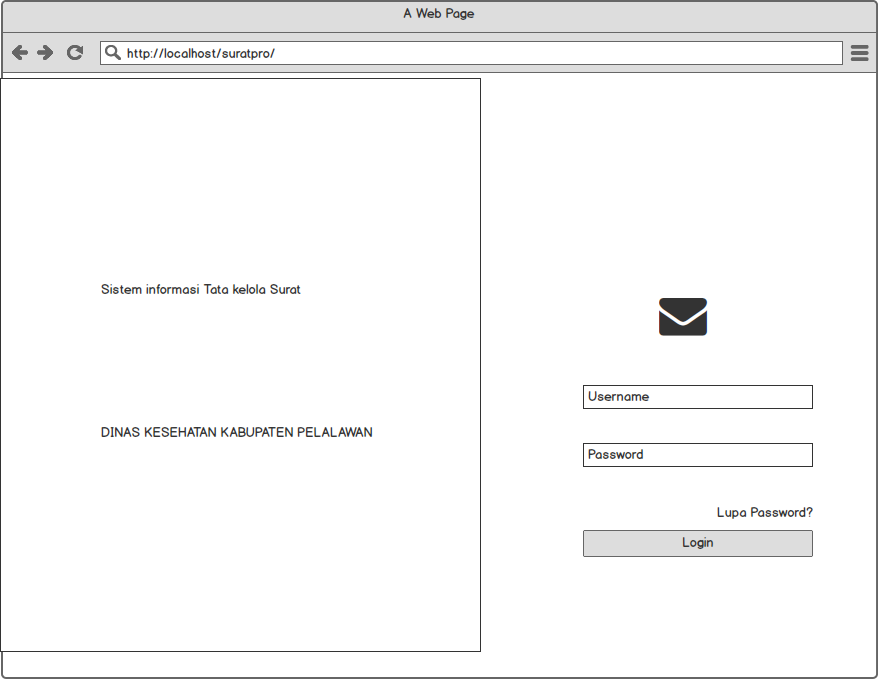
\includegraphics [height= 7cm, width=9cm]{konten/gambar/WireFrameSistemSurat/Admin/HalamanLogin.png}
			\caption{Halaman Login}
			\label{HalamanLogin}
		\end{figure}
		
		\item Dashboard
		
		Halaman dashboard dapat dilihat pada \pic\ref{HalamanDashboard1}
		
		pada halaman dashboard, terdapat beberapa menu, sesuai level user yang login, dalam hal ini adalah admin. Pada level admin, terdapat menu Agenda, Surat masuk , cetak laporan dan lain-lain. 
		\begin{figure}
			\centering
			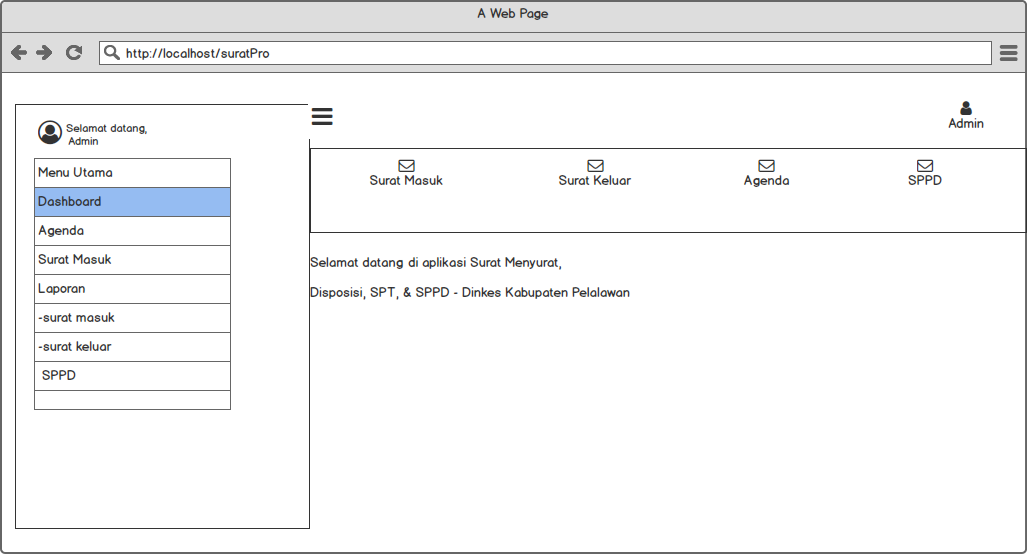
\includegraphics [height= 7cm, width=11cm]{konten/gambar/WireFrameSistemSurat/Admin/DashBoard.png}
			\caption{Halaman Dashboard}
			\label{HalamanDashboard1}
		\end{figure}
		
		\item Menu Master Golongan
		
		Halaman Menu Master Golongan dapat dilihat pada \pic\ref{HalamanInputMasterGolongan}
		
		\begin{figure}
			\centering
			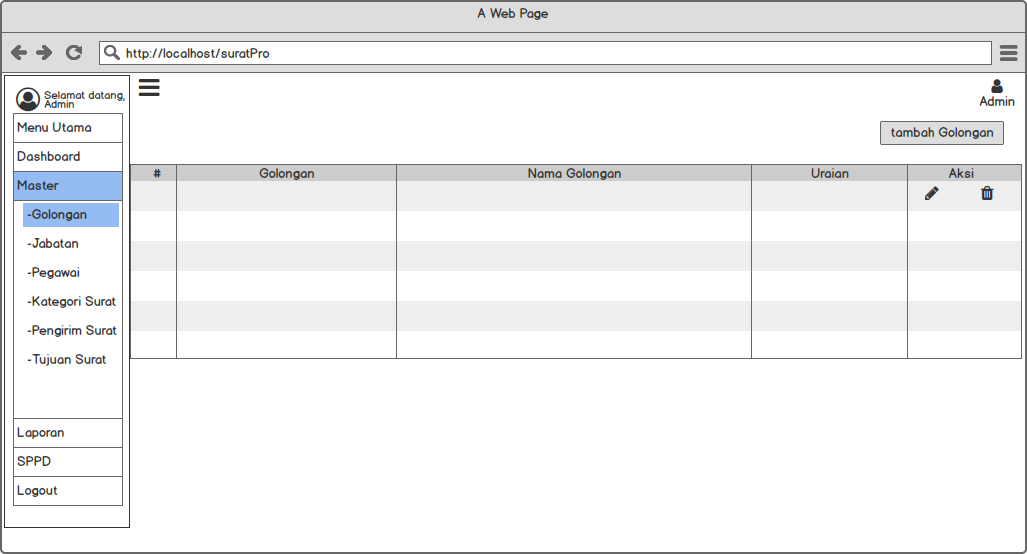
\includegraphics [height= 7cm, width=11cm]{konten/gambar/WireFrameSistemSurat/Admin/Mastergolongan.png}
			\caption{Halaman Input Master Golongan}
			\label{HalamanInputMasterGolongan}
		\end{figure}
		
		\item Menu Master Jabatan
		
		Halaman Input Master Jabatan dapat dilihat pada \pic\ref{HalamanInputMasterJabatan}
		
		\begin{figure}
			\centering
			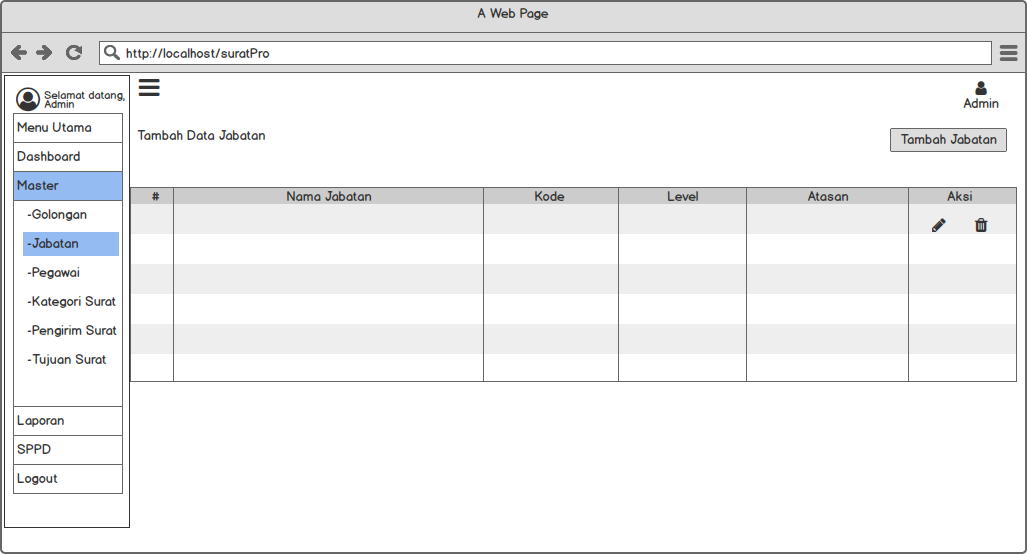
\includegraphics [height= 7cm, width=11cm]{konten/gambar/WireFrameSistemSurat/Admin/MasterJabatan.png}
			\caption{Halaman Input Master Jabatan}
			\label{HalamanInputMasterJabatan}
		\end{figure}
		
		\item Menu Master Pegawai
		
		Halaman Input Master Pegawai dapat dilihat pada \pic\ref{HalamanInputMasterPegawai}
		
		\begin{figure}
			\centering
			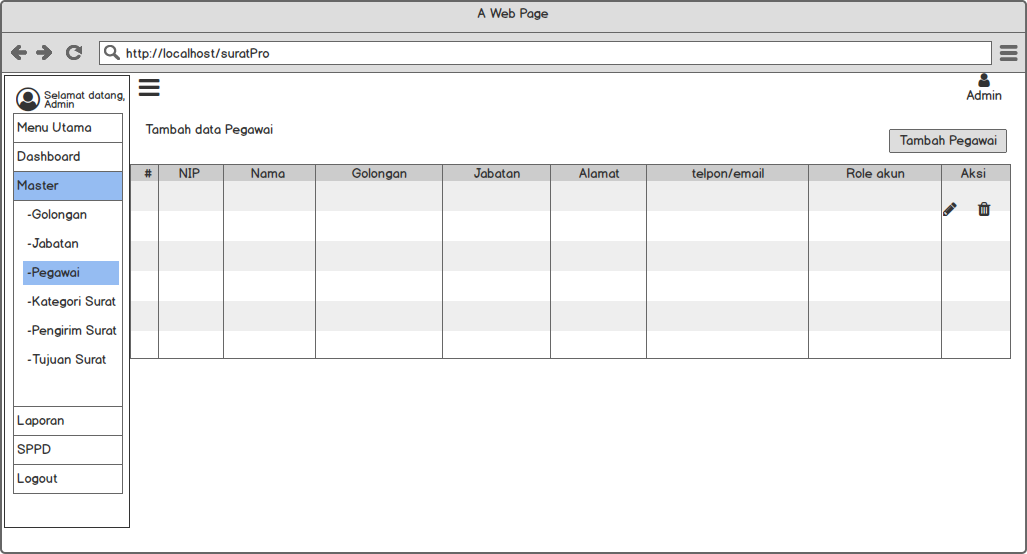
\includegraphics [height= 7cm, width=11cm]{konten/gambar/WireFrameSistemSurat/Admin/MasterPegawai.png}
			\caption{Halaman Input Master Pegawai}
			\label{HalamanInputMasterPegawai}
		\end{figure}
		
		\item Menu Master Kategori Surat
		
		Halaman Menu Master Kategori Surat dapat dilihat pada \pic\ref{HalamanInputKategoriSurat}
		
		\begin{figure}
			\centering
			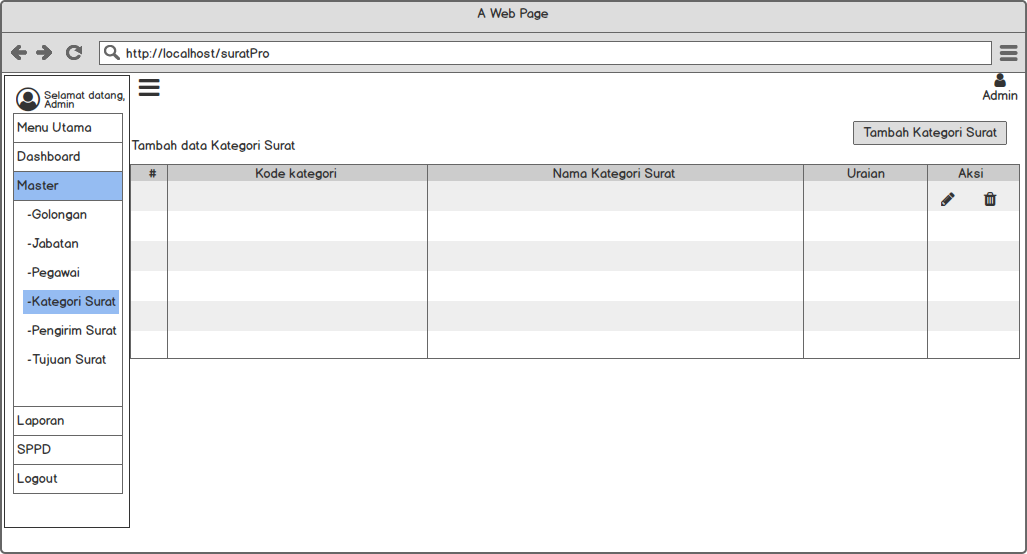
\includegraphics [height= 7cm, width=11cm]{konten/gambar/WireFrameSistemSurat/Admin/MasterKategoriSurat.png}
			\caption{Halaman Input Kategori Surat}
			\label{HalamanInputKategoriSurat}
		\end{figure}
		
		\item Menu Master Pengirim Surat
		
		Halaman Menu Master Pengirim Surat dapat dilihat pada \pic\ref{HalamanInputMasterPegawai}
		
		\begin{figure}
			\centering
			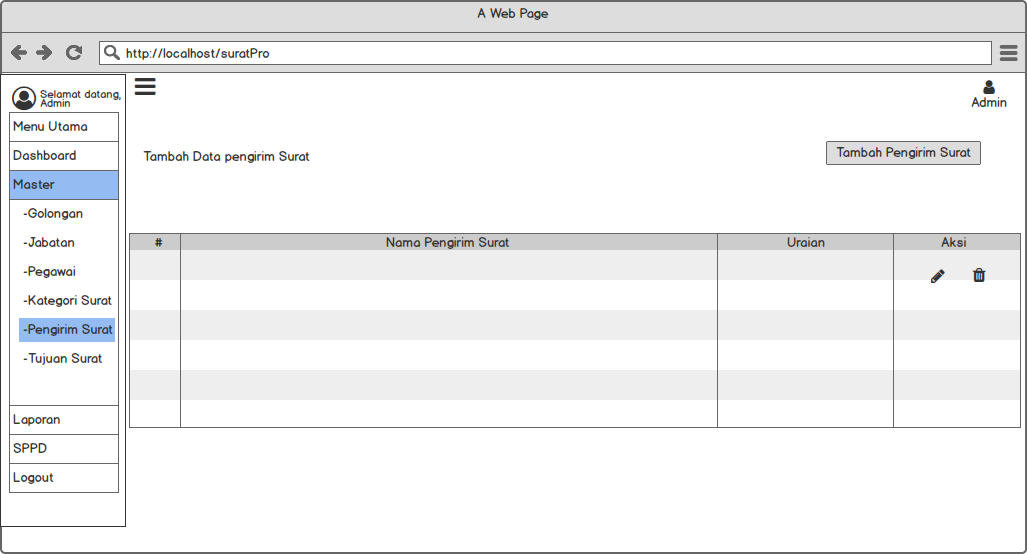
\includegraphics [height= 7cm, width=11cm]{konten/gambar/WireFrameSistemSurat/Admin/MasterPengirimSurat.png}
			\caption{Halaman Input Pengirim Surat}
			\label{HalamanInputPengirimSurat}
		\end{figure}
		
		\item Menu Master Tujuan Surat
		
		Halaman Menu Master Tujuan Surat dapat dilihat pada \pic\ref{HalamanInputTujuanSurat}
		
		\begin{figure}
			\centering
			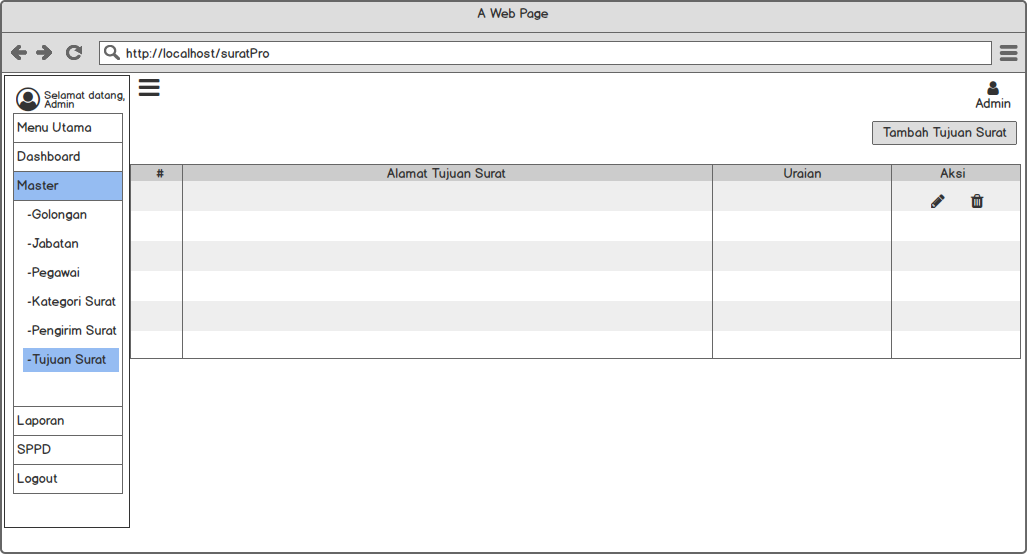
\includegraphics [height= 7cm, width=11cm]{konten/gambar/WireFrameSistemSurat/Admin/MasterTujuanSurat.png}
			\caption{Halaman Input Tujuan Surat}
			\label{HalamanInputTujuanSurat}
		\end{figure}
		
		\item Menu Laporan Surat Masuk
		
		Halaman Menu Laporan Surat Masuk  dapat dilihat pada \pic\ref{HalamanCetakLaporanSuratMasuk}
		
		\begin{figure}
			\centering
			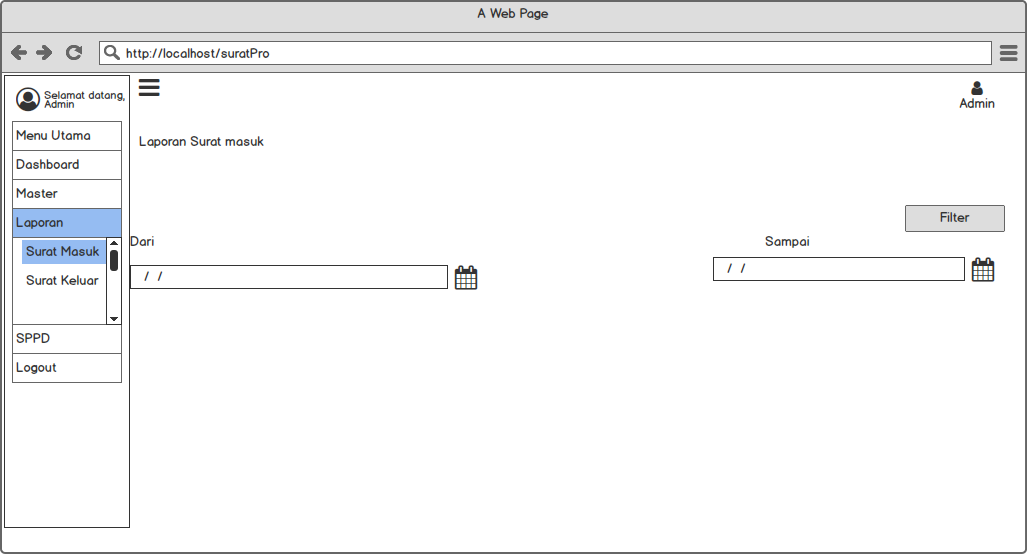
\includegraphics [height= 7cm, width=11cm]{konten/gambar/WireFrameSistemSurat/Admin/LaporanSuratMasuk.png}
			\caption{Halaman Cetak Laporan Surat Masuk}
			\label{HalamanCetakLaporanSuratMasuk}
		\end{figure}
		
		\item Menu Laporan Surat Keluar
		
		Halaman Menu Laporan Surat Keluar  dapat dilihat pada \pic\ref{HalamanCetakLaporanSuratKeluar}
		
		\begin{figure}
			\centering
			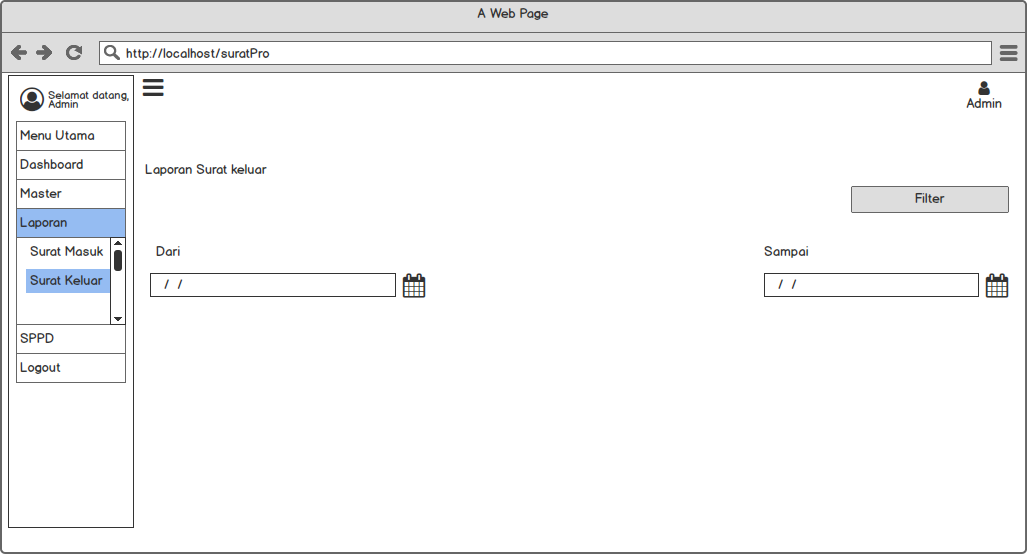
\includegraphics [height= 7cm, width=11cm]{konten/gambar/WireFrameSistemSurat/Admin/LaporanSuratKeluar.png}
			\caption{Halaman Cetak Laporan Surat Keluar}
			\label{HalamanCetakLaporanSuratKeluar}
		\end{figure}
		
		\item Menu SPPD Master Kegiatan
		
		Halaman Menu SPPD Master Kegiatan  dapat dilihat pada \pic\ref{HalamanLihatMasterSPPD}
		
		\begin{figure}
			\centering
			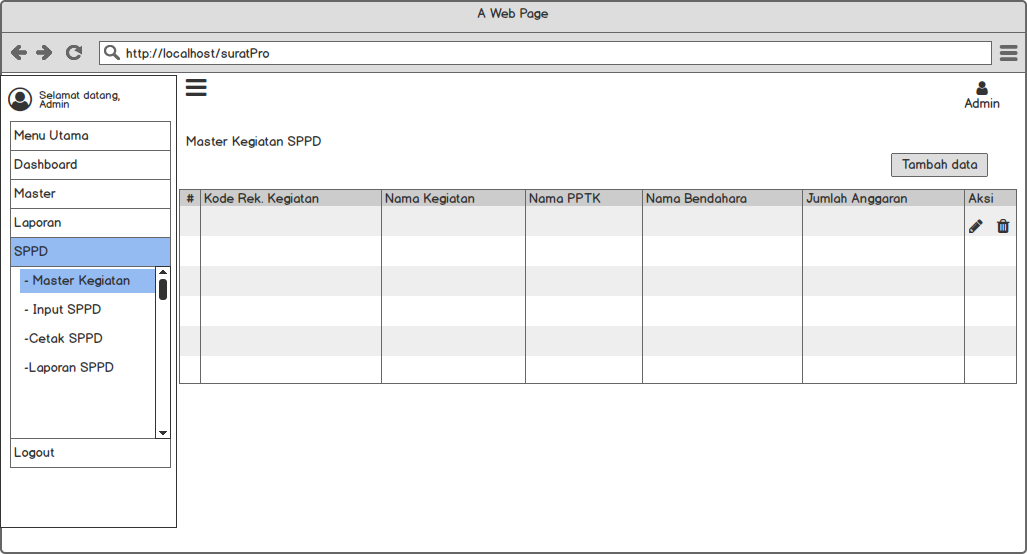
\includegraphics [height= 7cm, width=11cm]{konten/gambar/WireFrameSistemSurat/Admin/MasterkegiatanSPPD.png}
			\caption{Halaman Lihat Master SPPD}
			\label{HalamanLihatMasterSPPD}
		\end{figure}
		
		\item Menu SPPD Input SPPD
		
		Halaman Menu SPPD Input SPPD  dapat dilihat pada \pic\ref{HalamanInputMasterSPPD}
		
		\begin{figure}
			\centering
			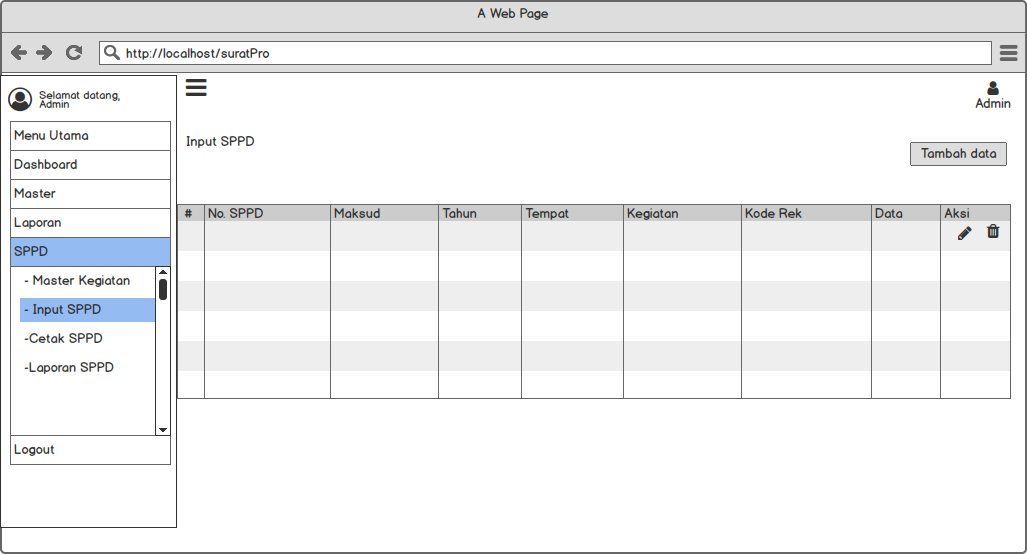
\includegraphics [height= 7cm, width=11cm]{konten/gambar/WireFrameSistemSurat/Admin/InputSPPD.png}
			\caption{Halaman Input Master SPPD}
			\label{HalamanInputMasterSPPD}
		\end{figure}
		
		\item Menu SPPD Cetak SPPD
		
		Halaman Menu SPPD Cetak SPPD  dapat dilihat pada \pic\ref{HalamanCetakSPPD}
		
		\begin{figure}
			\centering
			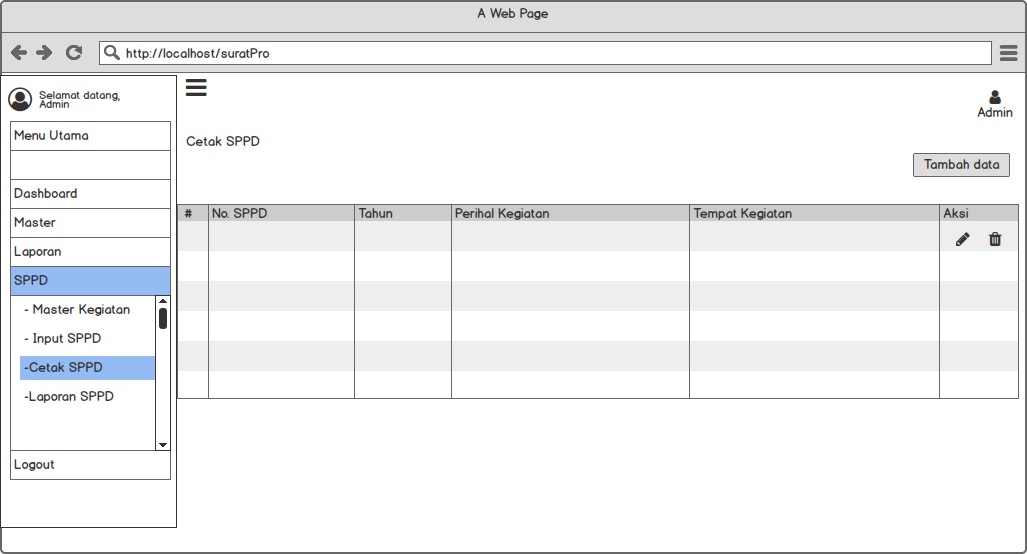
\includegraphics [height= 7cm, width=11cm]{konten/gambar/WireFrameSistemSurat/Admin/CetakSPPD.png}
			\caption{Halaman Cetak SPPD}
			\label{HalamanCetakSPPD}
		\end{figure}
		
		\item Menu Laporan SPPD
		
		Halaman Menu Laporan SPPD dapat dilihat pada \pic\ref{HalamanLihatLaporanSPPD}
		
		\begin{figure}
			\centering
			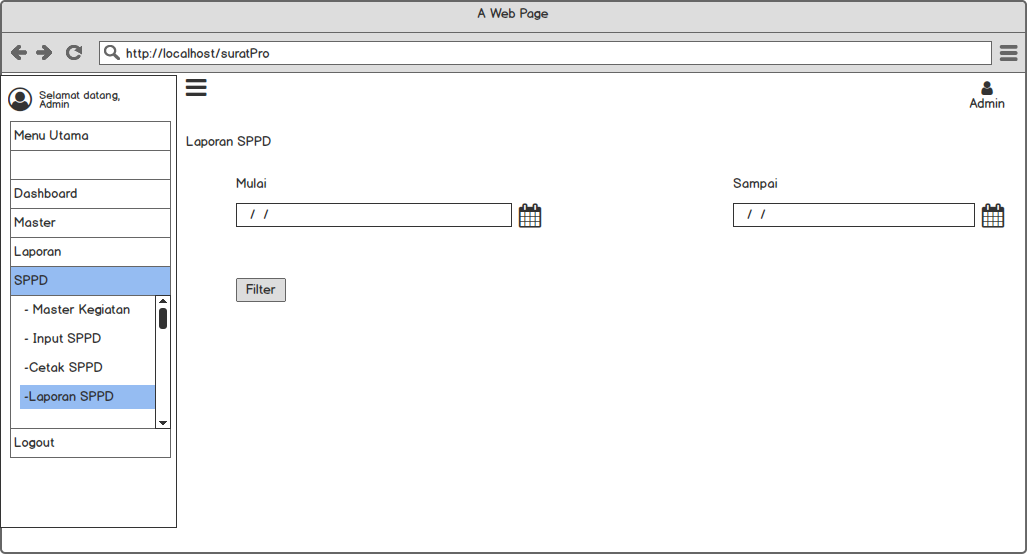
\includegraphics [height= 7cm, width=11cm]{konten/gambar/WireFrameSistemSurat/Admin/LaporanSPPD.png}
			\caption{Halaman Lihat Laporan SPPD}
			\label{HalamanLihatLaporanSPPD}
		\end{figure}
	\end{enumerate}
	
	\item Desagin Antar Muka Kadis
	
	\begin{enumerate}
		\item Dashboard
		
		Halaman Dashboard Kadis dapat dilihat pada \pic~\ref{HalamanDashboardKadis}.
		\begin{figure}
			\centering
			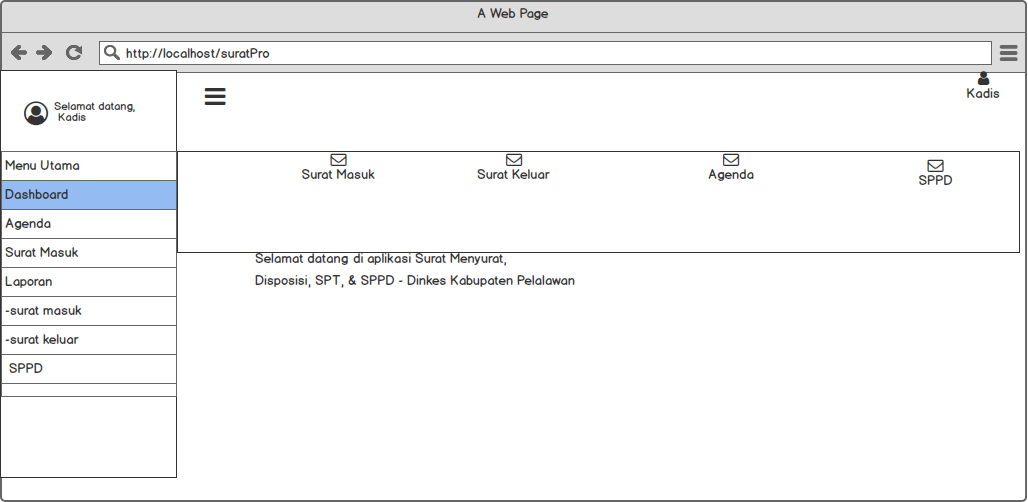
\includegraphics [height= 7cm, width=11cm]{konten/gambar/WireFrameSistemSurat/Kadis/DashBoard.png}
			\caption{Halaman Dashboard}
			\label{HalamanDashboardKadis}
		\end{figure}
		
		\item Menu Master Golongan
		
		Halaman Menu Master Golongan dapat dilihat pada \pic~\ref{HalamanLihatDaftarAgendaKadis}
		
		\begin{figure}
			\centering
			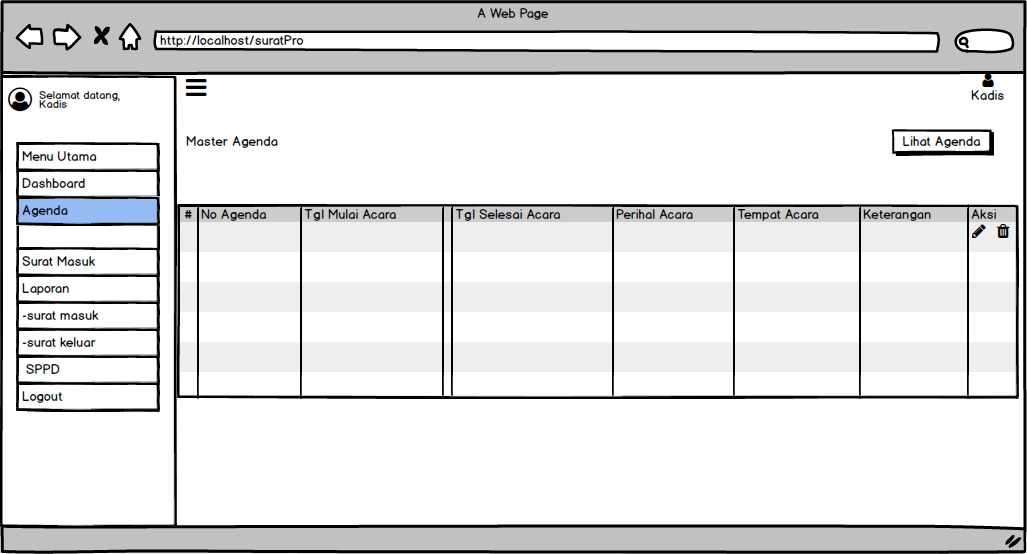
\includegraphics [height= 7cm, width=11cm]{konten/gambar/WireFrameSistemSurat/Kadis/DaftarAgenda.png}
			\caption{Halaman Lihat Daftar Agenda}
			\label{HalamanLihatDaftarAgendaKadis}
		\end{figure}
		
		\item Menu Master Jabatan
		
		Halaman Menu Master Golongan dapat dilihat pada \pic~\ref{HalamanLihatDaftarAgendaKadis}
		
		\begin{figure}
			\centering
			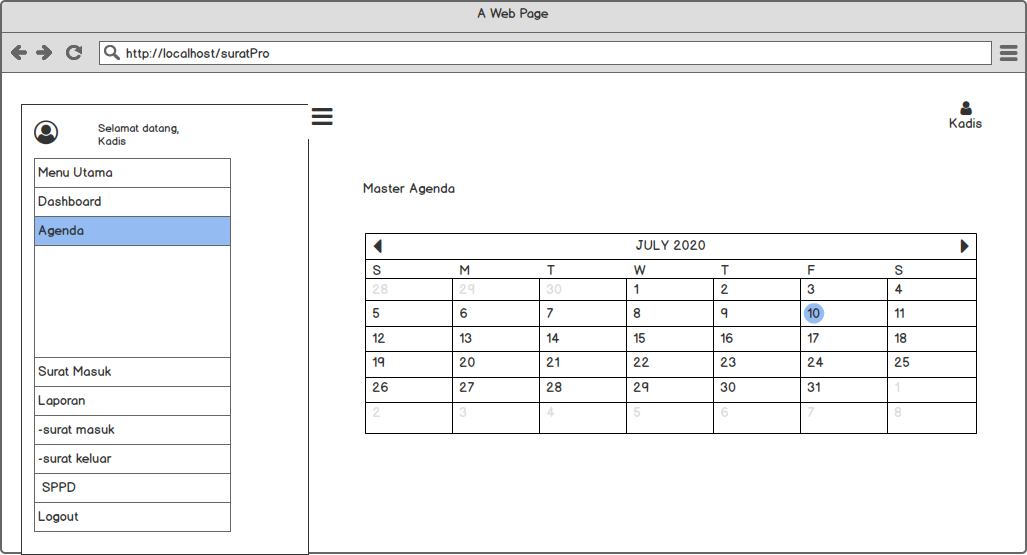
\includegraphics [height= 7cm, width=11cm]{konten/gambar/WireFrameSistemSurat/Kadis/TampilanAgendakalender.png}
			\caption{Tampilan Agenda Di Kalender}
			\label{HalamanTampilanAgendakalender}
		\end{figure}
		
		\item Menu Master Pegawai
		
		Halaman Menu Master Pegawai dapat dilihat pada \pic~\ref{HalamanSuratMasuk}
		
		\begin{figure}
			\centering
			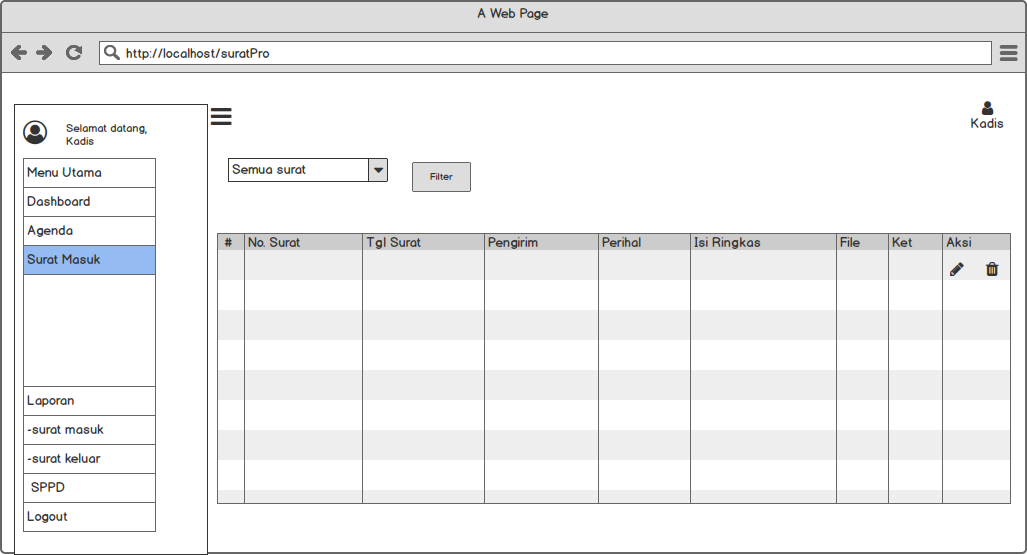
\includegraphics [height= 7cm, width=11cm]{konten/gambar/WireFrameSistemSurat/Kadis/SuratMasuk.png}
			\caption{Halaman Surat Masuk}
			\label{HalamanSuratMasuk}
		\end{figure}
		
		\item Menu Master Kategori Surat 
		
		Halaman Menu Master Kategori Surat dapat dilihat pada \pic~\ref{HalamanLaporanSuratMasukKadis}
		
		\begin{figure}
			\centering
			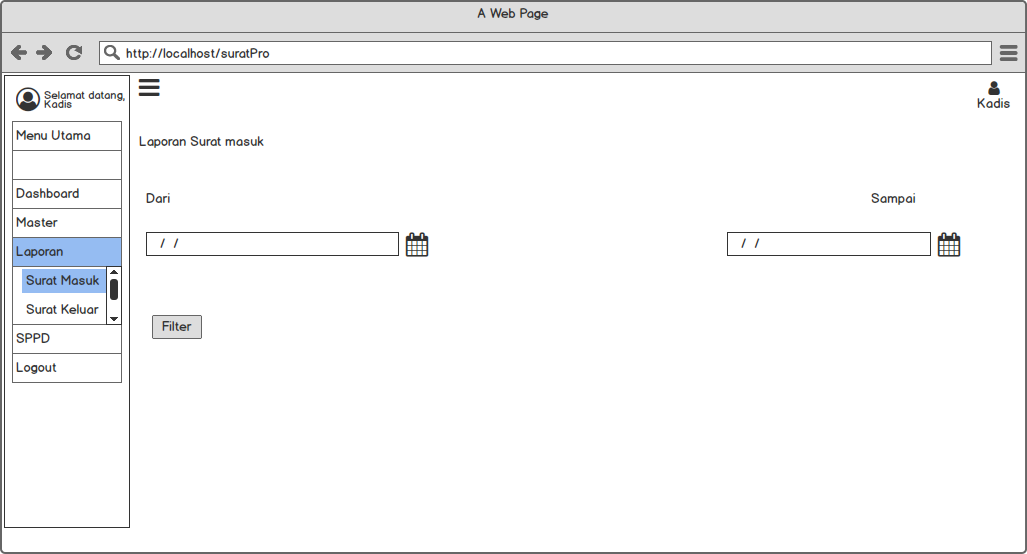
\includegraphics [height= 7cm, width=11cm]{konten/gambar/WireFrameSistemSurat/Kadis/LaporanSuratMasuk.png}
			\caption{Halaman Laporan Surat Masuk}
			\label{HalamanLaporanSuratMasukKadis}
		\end{figure}
		
		\item Menu Master Pengirim Surat
		
		Halaman Menu Master Pengirim Surat dapat dilihat pada \pic~\ref{HalamanLaporanSuratKeluar}
		
		\begin{figure}
			\centering
			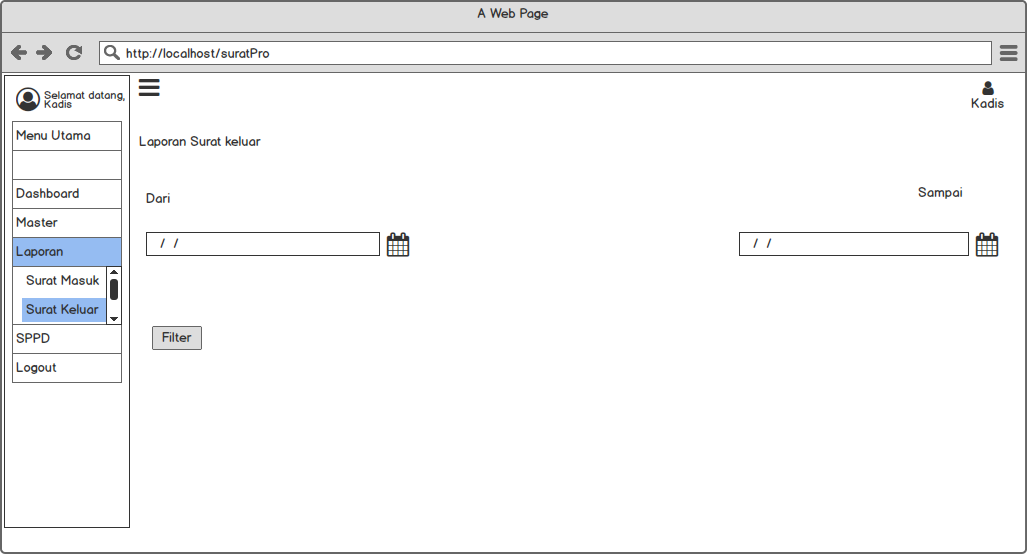
\includegraphics [height= 7cm, width=11cm]{konten/gambar/WireFrameSistemSurat/Kadis/LaporanSuratKeluar.png}
			\caption{Halaman Laporan Surat Keluar}
			\label{HalamanLaporanSuratKeluar}
		\end{figure}
		
		\item Menu SPPD Master Kegiatan
		
		Halaman Menu SPPD Master Kegiatan dapat dilihat pada \pic~\ref{HalamanLihatMasterSPPDKadis}
		
		\begin{figure}
			\centering
			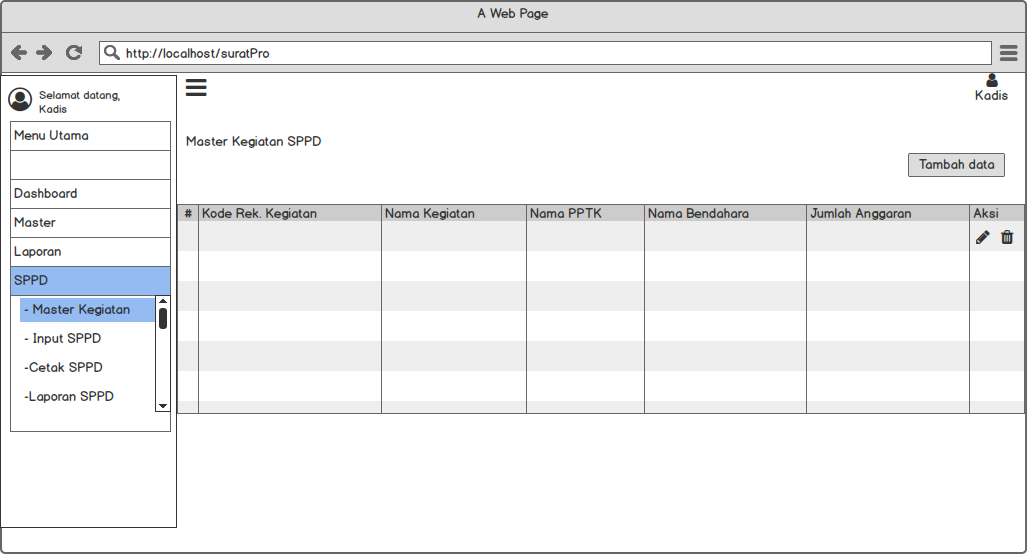
\includegraphics [height= 7cm, width=11cm]{konten/gambar/WireFrameSistemSurat/Kadis/MasterkegiatanSPPD.png}
			\caption{Halaman Lihat Master SPPD}
			\label{HalamanLihatMasterSPPDKadis}
		\end{figure}
		
		\item Menu SPPD Input SPPD
		
		Halaman Menu SPPD Input SPPD dapat dilihat pada \pic~\ref{HalamanInputMasterSPPDKadis}
		
		\begin{figure}
			\centering
			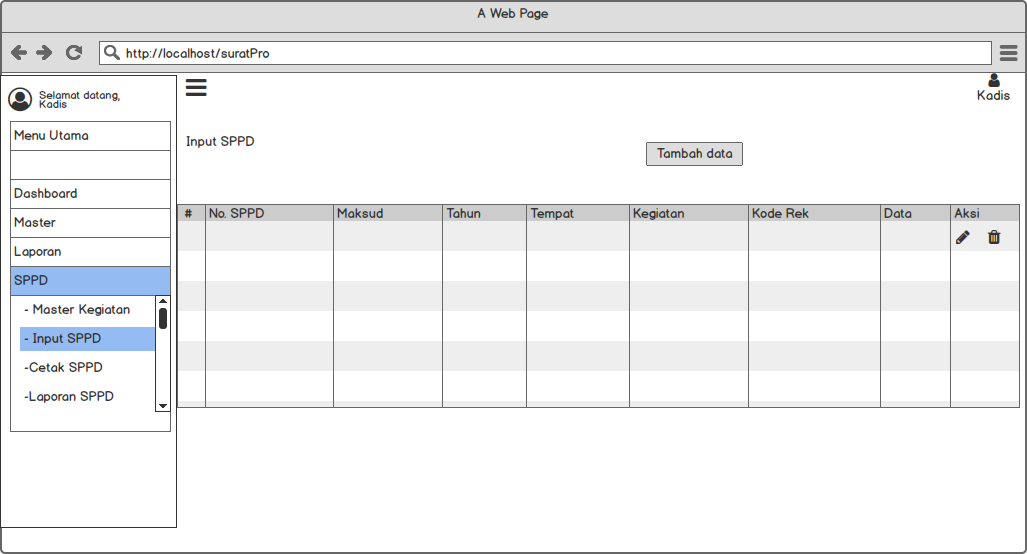
\includegraphics [height= 7cm, width=11cm]{konten/gambar/WireFrameSistemSurat/Kadis/InputSPPD.png}
			\caption{Halaman Input Master SPPD}
			\label{HalamanInputMasterSPPDKadis}
		\end{figure}
		
		\item Menu SPPD Cetak SPPD
		
		Halaman Menu SPPD Cetak SPPD dapat dilihat pada \pic~\ref{HalamanCetakSPPDKadis}
		
		\begin{figure}
			\centering
			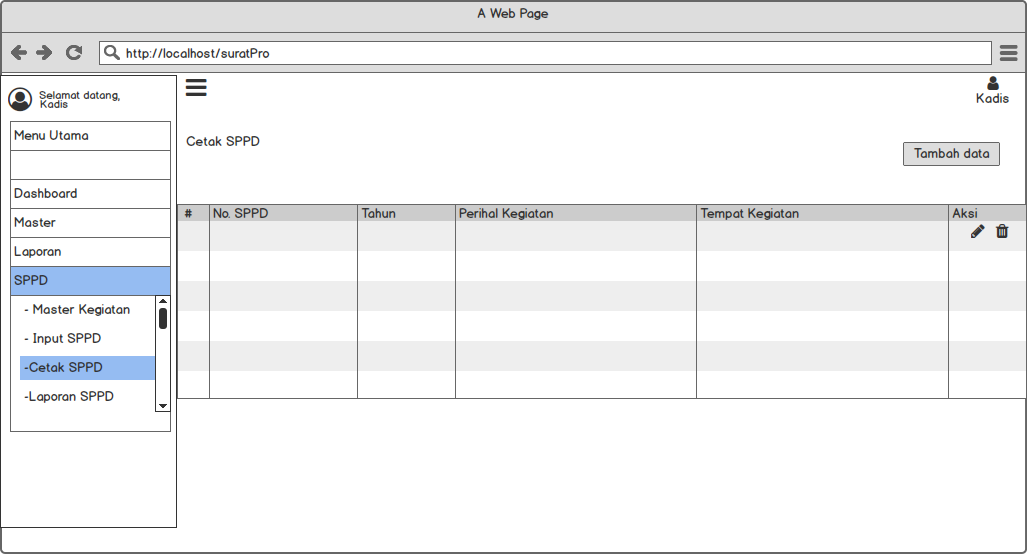
\includegraphics [height= 7cm, width=11cm]{konten/gambar/WireFrameSistemSurat/Kadis/CetakSPPD.png}
			\caption{Halaman Cetak SPPD}
			\label{HalamanCetakSPPDKadis}
		\end{figure}
		
		\item Menu Laporan SPPD
		
		Halaman Menu Laporan SPPD dapat dilihat pada \pic~\ref{HalamanLihatLaporanSPPDKadis}
		
		\begin{figure}
			\centering
			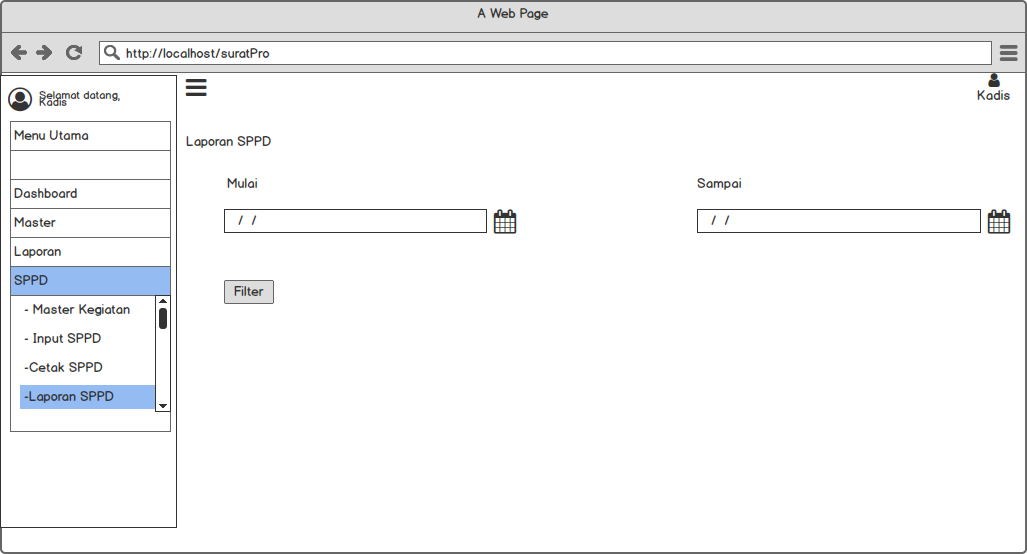
\includegraphics [height= 7cm, width=11cm]{konten/gambar/WireFrameSistemSurat/Kadis/LaporanSPPD.png}
			\caption{Halaman Lihat Laporan SPPD}
			\label{HalamanLihatLaporanSPPDKadis}
		\end{figure}
		
	\end{enumerate}
	
\item Desagin Antar Muka Pengagenda
	
	\begin{enumerate}
		\item Halaman Dashboard
		
		Halaman Desagin Dashboard dapat dilihat pada \pic~\ref{HalamanDashBoardPengagenda}
		
		\begin{figure}
			\centering
			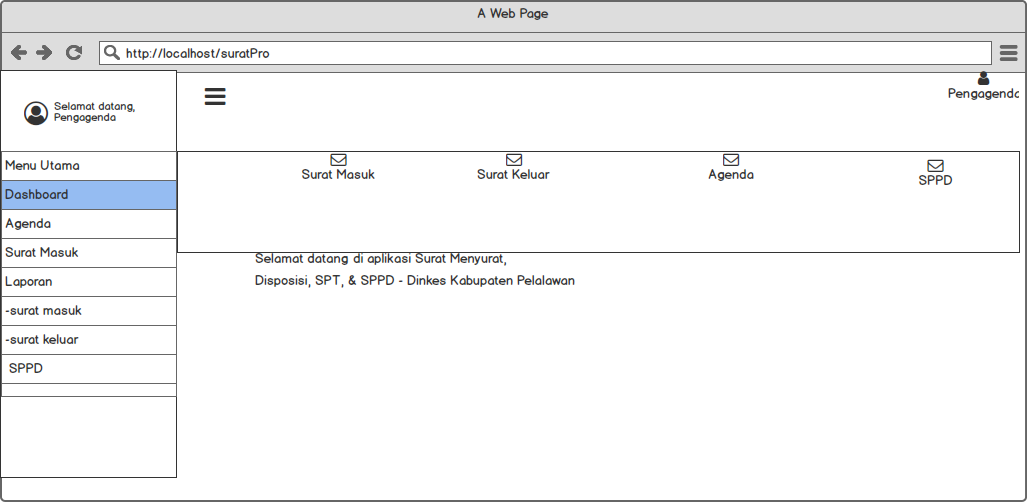
\includegraphics [height= 7cm, width=11cm]{konten/gambar/WireFrameSistemSurat/Pengagenda/DashBoard.png}
			\caption{Halaman DashBoard Pengagenda}
			\label{HalamanDashBoardPengagenda}
		\end{figure}
		
		\item Halaman Daftar Agenda
		
		Halaman Daftar Agenda dapat dilihat pada \pic~\ref{HalamanDaftarAgenda}.
		
		\begin{figure}
			\centering
			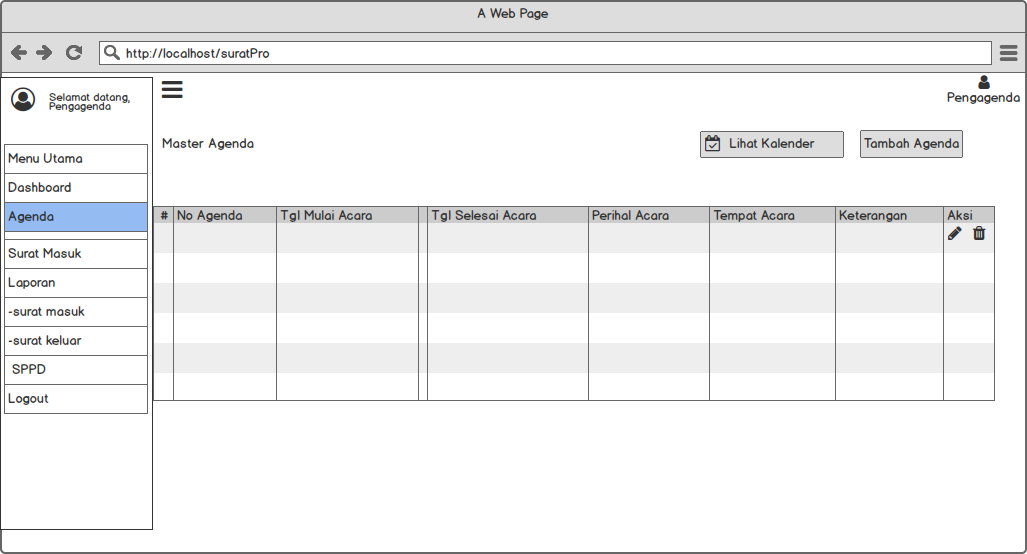
\includegraphics [height= 7cm, width=11cm]{konten/gambar/WireFrameSistemSurat/Pengagenda/DaftarAgenda.png}
			\caption{Halaman Daftar Agenda Pengagenda}
			\label{HalamanDaftarAgenda}
		\end{figure}
		
		\item Halaman Tampilan Agenda kalender Pengagenda
		
		Halaman Tampilan Agenda dapat dilihat pada \pic~\ref{HalamanTampilankalenderPengagenda}
		
		\begin{figure}
			\centering
			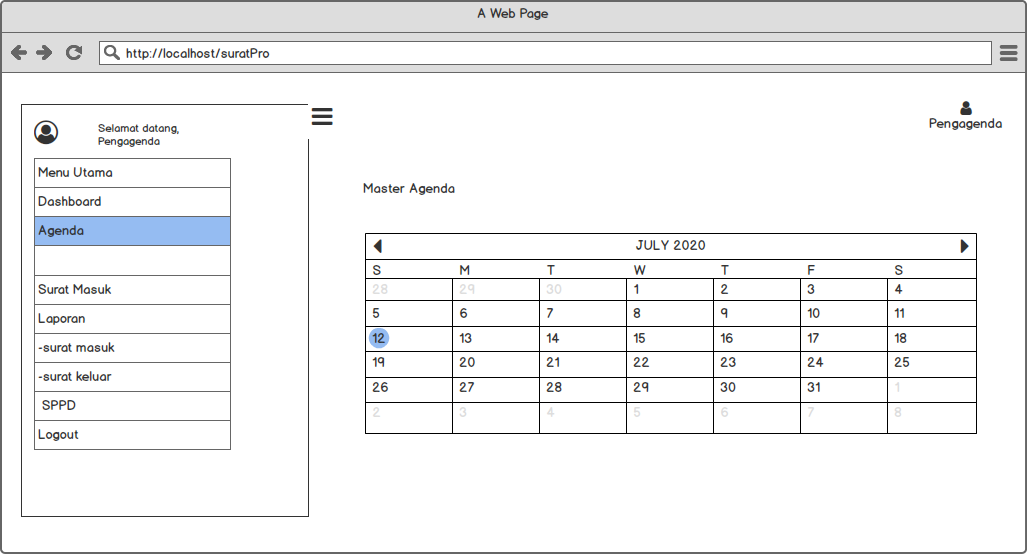
\includegraphics [height= 7cm, width=11cm]{konten/gambar/WireFrameSistemSurat/Pengagenda/TampilanAgendakalender.png}
			\caption{Halaman Tampilan Agenda kalender Pengagenda}
			\label{HalamanTampilankalenderPengagenda}
		\end{figure}
		
		\item Halaman Tampilan Tambah Agenda Kalender Pengagenda
		
		Halaman Tampilan Tambah Agenda Kalender Pengagenda dapat dilihat pada \pic~\ref{TampilanTambahAgendakalenderPenagenda}
		
		\begin{figure}
			\centering
			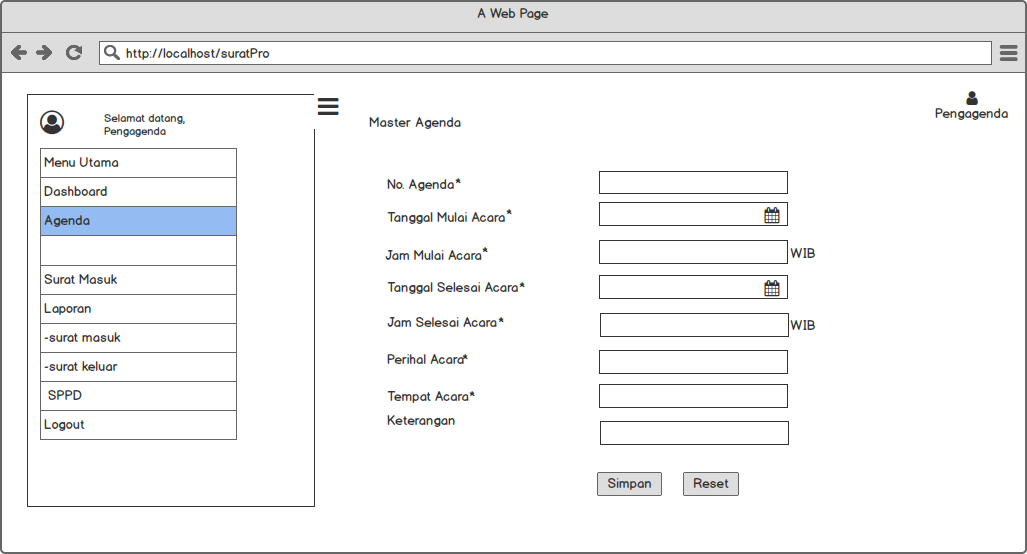
\includegraphics [height= 7cm, width=11cm]{konten/gambar/WireFrameSistemSurat/Pengagenda/TampilanTambahAgendakalender.png}
			\caption{Halaman Tampilan Tambah Agenda Kalender Pengagenda}
			\label{TampilanTambahAgendakalenderPenagenda}
		\end{figure}
		
		\item Halaman Surat Masuk Pengagenda
		
		Halaman Halaman Surat Masuk Pengagenda dapat dilihat pada \pic~\ref{HalamanSuratMasukPengagenda}
		
		\begin{figure}
			\centering
			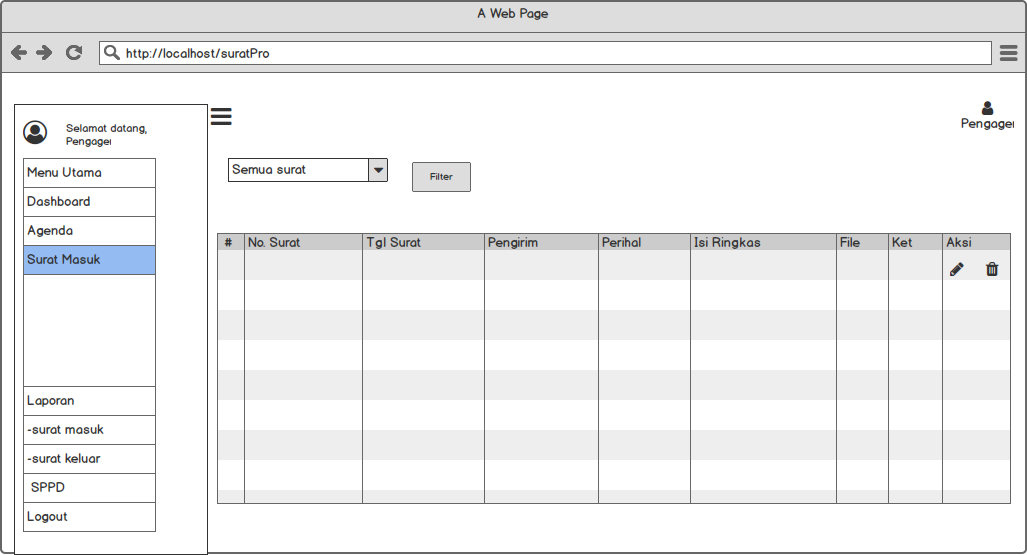
\includegraphics [height= 7cm, width=11cm]{konten/gambar/WireFrameSistemSurat/Pengagenda/SuratMasuk.png}
			\caption{Halaman Surat Masuk Pengagenda}
			\label{HalamanSuratMasukPengagenda}
		\end{figure}
		
		\item Halaman Laporan Surat Masuk Pengagenda
		
		Halaman Laporan Surat Masuk Pengagenda dapat dilihat pada \pic~\ref{HalamanLaporanSuratMasukPengagenda}
		
		\begin{figure}
			\centering
			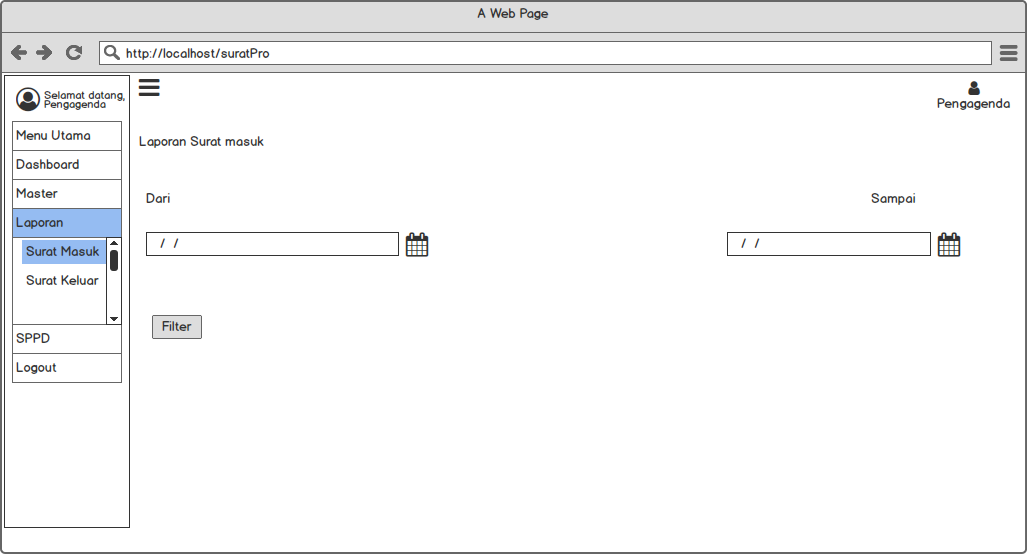
\includegraphics [height= 7cm, width=11cm]{konten/gambar/WireFrameSistemSurat/Pengagenda/LaporanSuratMasuk.png}
			\caption{Halaman Laporan Surat Masuk Pengagenda}
			\label{HalamanLaporanSuratMasukPengagenda}
		\end{figure}
		
		\item Halaman Laporan Surat Keluar Pengagenda
		
		Halaman Laporan Surat Keluar Pengagenda dapat dilihat pada \pic~\ref{LaporanSuratKeluarPengagenda}
		
		\begin{figure}
			\centering
			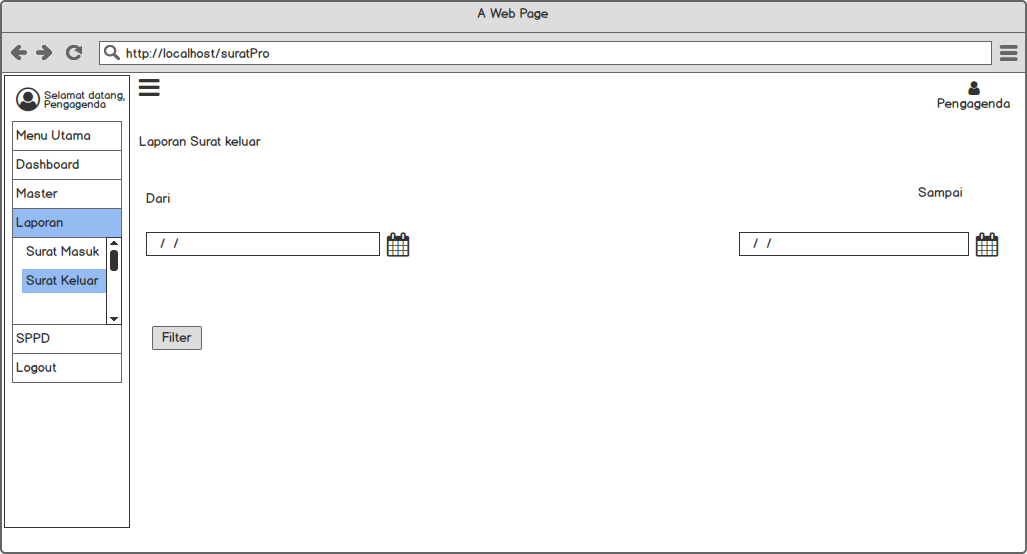
\includegraphics [height= 7cm, width=11cm]{konten/gambar/WireFrameSistemSurat/Pengagenda/LaporanSuratKeluar.png}
			\caption{Halaman Laporan Surat Keluar Pengagenda}
			\label{LaporanSuratKeluarPengagenda}
		\end{figure}
		
		\item Halaman Lihat Master SPPD Pengagenda
		
		Halaman Lihat Master SPPD Pengagenda dapat dilihat pada \pic~\ref{HalamanLihatMasterSPPDPengagenda}
		
		\begin{figure}
			\centering
			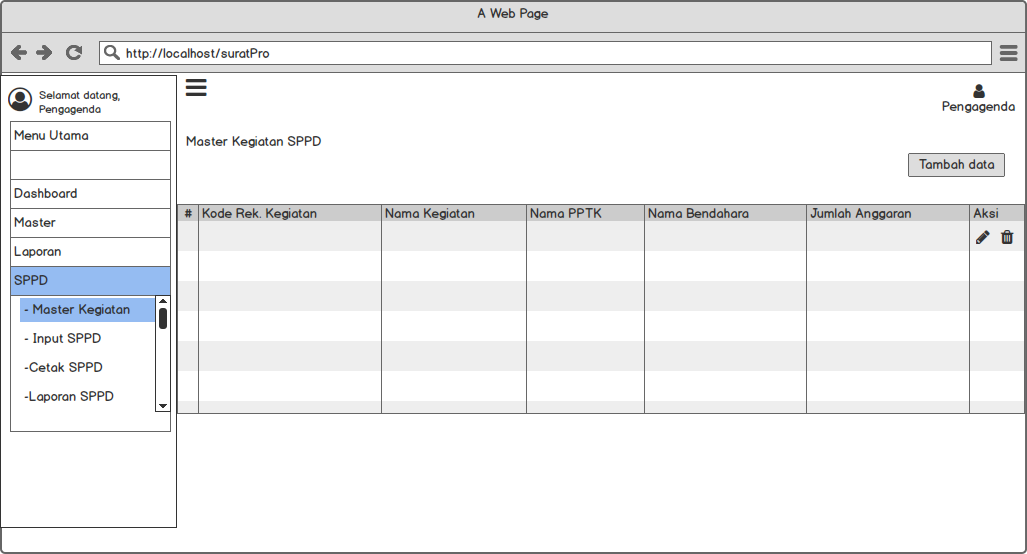
\includegraphics [height= 7cm, width=11cm]{konten/gambar/WireFrameSistemSurat/Pengagenda/MasterkegiatanSPPD.png}
			\caption{Halaman Lihat Master SPPD Pengagenda}
			\label{HalamanLihatMasterSPPDPengagenda}
		\end{figure}
		
		\item Halaman Input Master SPPD Pengagenda
		
		Halaman Input Master SPPD Pengagenda dapat dilihat pada \pic~\ref{HalamanInputMasterSPPDPengagenda}
		
		\begin{figure}
			\centering
			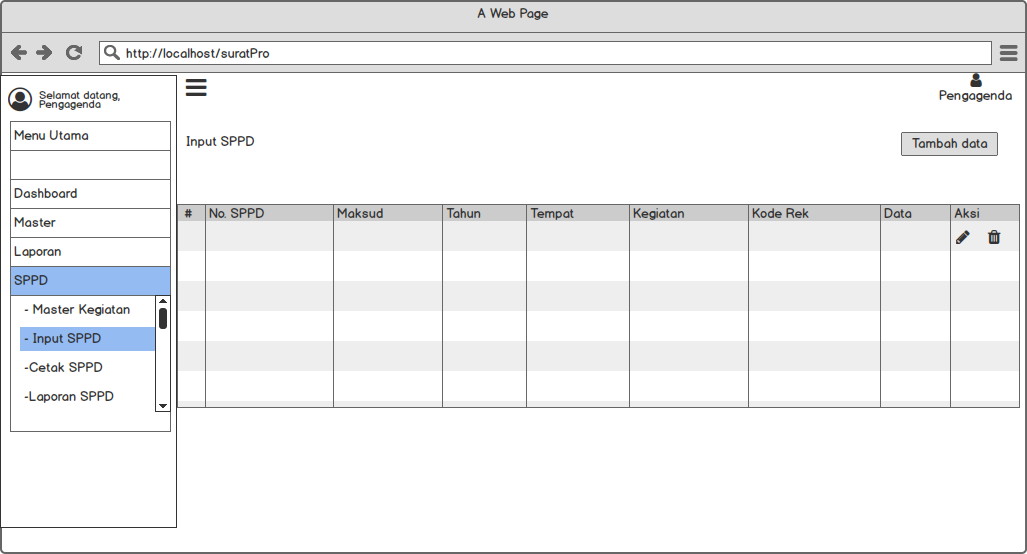
\includegraphics [height= 7cm, width=11cm]{konten/gambar/WireFrameSistemSurat/Pengagenda/InputSPPD.png}
			\caption{Halaman Input Master SPPD Pengagenda}
			\label{HalamanInputMasterSPPDPengagenda}
		\end{figure}
		
		\item Halaman Cetak SPPD Pengagenda
		
		Halaman Cetak SPPD Pengagenda dapat dilihat pada \pic~\ref{HalamanCetakSPPDPengagenda}
		
		\begin{figure}
			\centering
			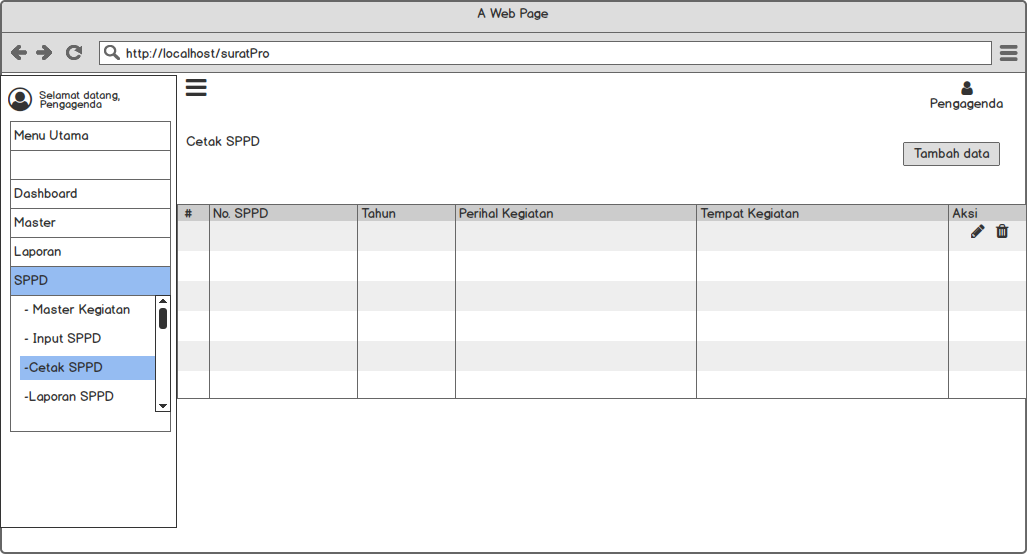
\includegraphics [height= 7cm, width=11cm]{konten/gambar/WireFrameSistemSurat/Pengagenda/CetakSPPD.png}
			\caption{Halaman Cetak SPPD Pengagenda}
			\label{HalamanCetakSPPDPengagenda}
		\end{figure}
		
		\item Halaman Cetak SPPD Pengagenda
		
		Halaman Cetak SPPD Pengagenda dapat dilihat pada \pic~\ref{HalamanLaporanSPPDPengagenda}
		
		\begin{figure}
			\centering
			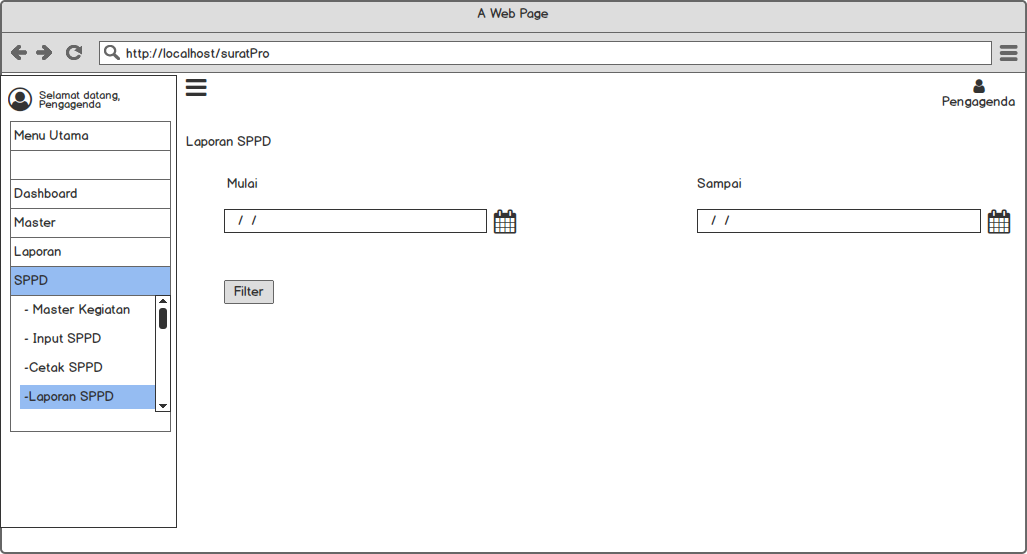
\includegraphics [height= 7cm, width=11cm]{konten/gambar/WireFrameSistemSurat/Pengagenda/LaporanSPPD.png}
			\caption{Halaman Cetak SPPD Pengagenda}
			\label{HalamanLaporanSPPDPengagenda}
		\end{figure}
		
	\end{enumerate}
	
	\item Desaign Antar Muka Pegawai
	
	\begin{enumerate}
		\item Halaman dashboard
		
		Halaman dashboard dapat dilihat pada \pic~\ref{HalamanDashBoardPegawai}
		
		\begin{figure}
			\centering
			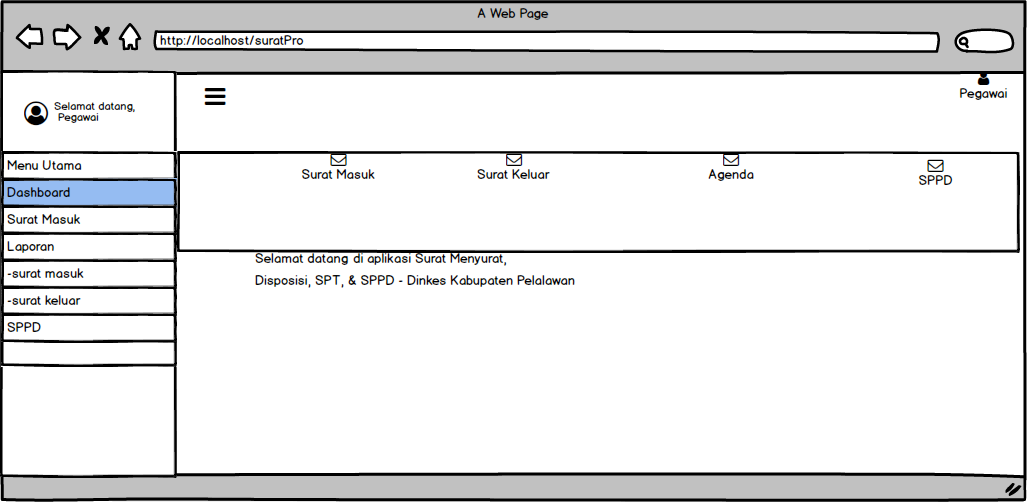
\includegraphics [height= 7cm, width=11cm]{konten/gambar/WireFrameSistemSurat/Pegawai/DashBoard.png}
			\caption{Halaman DashBoard Pegawai}
			\label{HalamanDashBoardPegawai}
		\end{figure}
		
		\item Halaman Surat Masuk
		
		Halaman Surat Masuk dapat dilihat pada \pic~\ref{HalamanSuratMasukPegawai}
		
		\begin{figure}
			\centering
			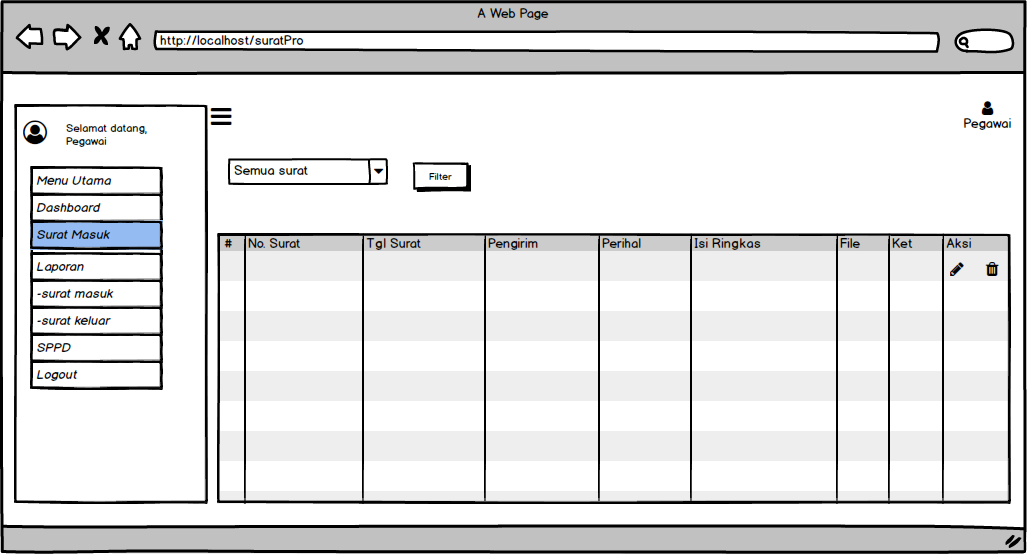
\includegraphics [height= 7cm, width=11cm]{konten/gambar/WireFrameSistemSurat/Pegawai/SuratMasuk.png}
			\caption{Halaman Surat Masuk Pegawai}
			\label{HalamanSuratMasukPegawai}
		\end{figure}
		
		\item Laporan Surat Masuk
		
		Laporan Surat Masuk dapat dilihat pada \pic~\ref{HalamanLaporanSuratMasukPegawai}
		
		\begin{figure}
			\centering
			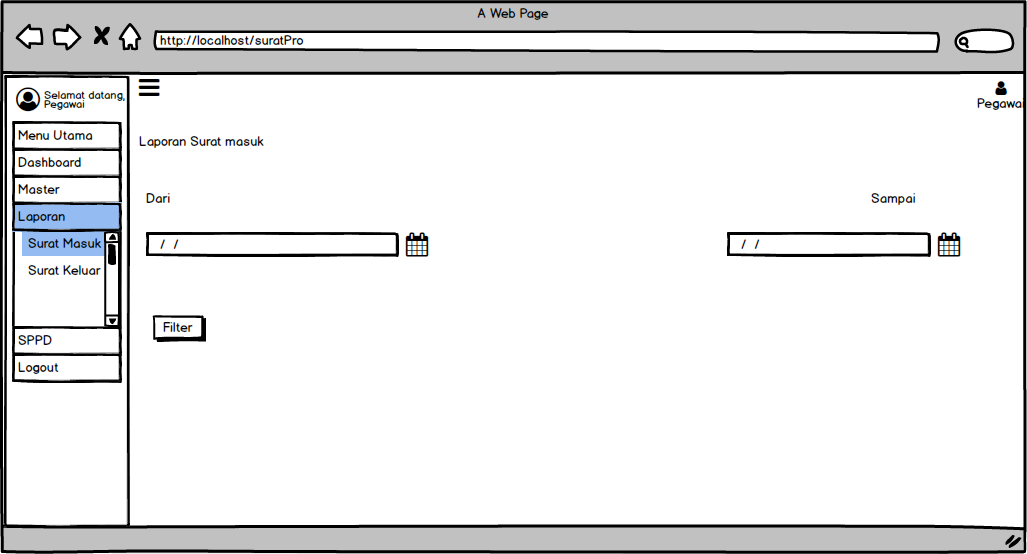
\includegraphics [height= 7cm, width=11cm]{konten/gambar/WireFrameSistemSurat/Pegawai/LaporanSuratMasuk.png}
			\caption{Halaman Laporan Surat Masuk Pegawai}
			\label{HalamanLaporanSuratMasukPegawai}
		\end{figure}
		
		\item Laporan Surat Keluar
		
		Laporan Surat Keluar dapat dilihat pada \pic~\ref{HalamanLaporanKeluarMasukPegawai}
		
		\begin{figure}
			\centering
			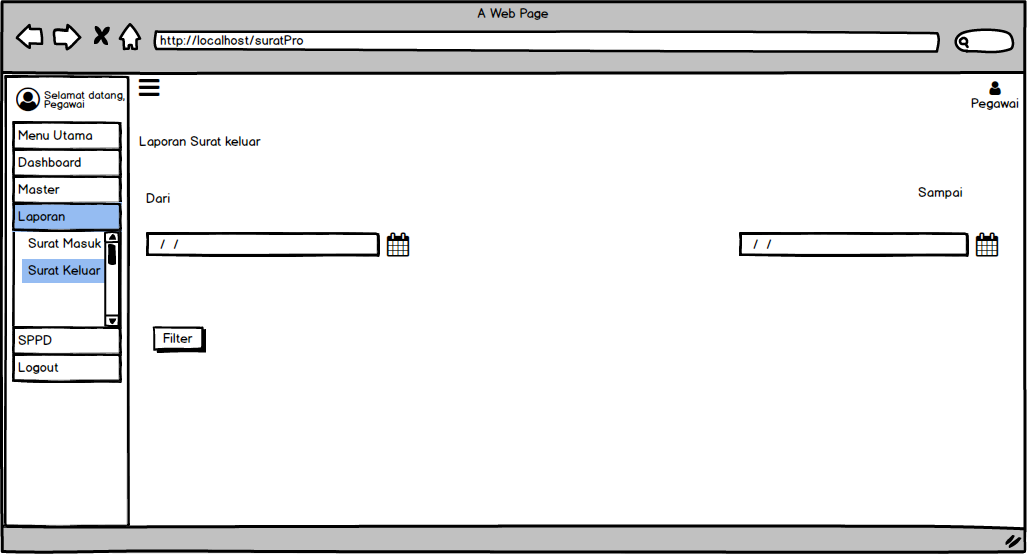
\includegraphics [height= 7cm, width=11cm]{konten/gambar/WireFrameSistemSurat/Pegawai/LaporanSuratKeluar.png}
			\caption{Halaman Laporan Surat Masuk Pegawai}
			\label{HalamanLaporanKeluarMasukPegawai}
		\end{figure}
		
		\item Laporan Master SPPD 
		
		Laporan Master SPPD dapat dilihat pada \pic~\ref{HalamanMasterkegiatanSPPDPegawai}
		
		\begin{figure}
			\centering
			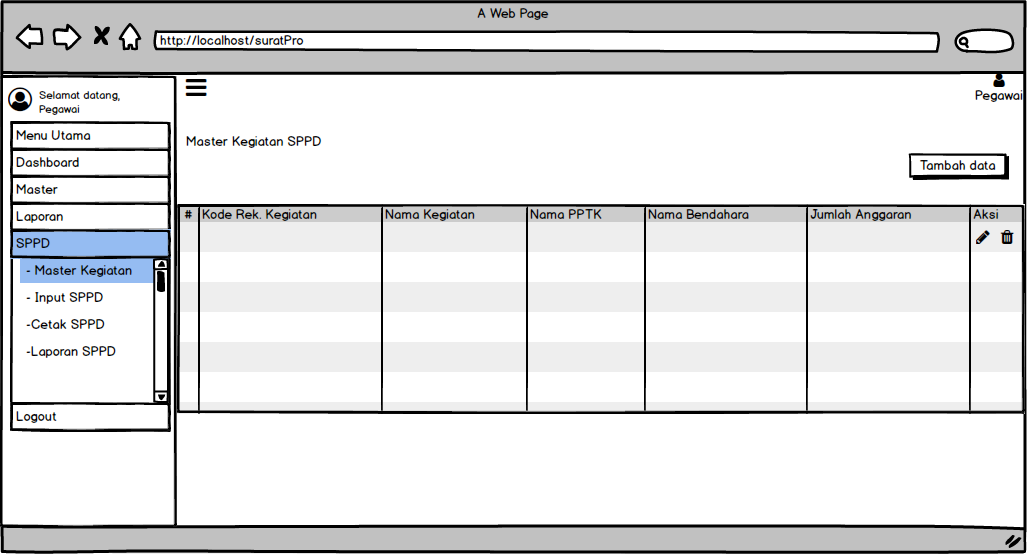
\includegraphics [height= 7cm, width=11cm]{konten/gambar/WireFrameSistemSurat/Pegawai/MasterkegiatanSPPD.png}
			\caption{Halaman Master kegiatan SPPD Pegawai}
			\label{HalamanMasterkegiatanSPPDPegawai}
		\end{figure}
		
		\item Laporan Input SPPD 
		
		Laporan Input SPPD  dapat dilihat pada \pic~\ref{HalamanHalamanInputSPPDPegawai}
		
		\begin{figure}
			\centering
			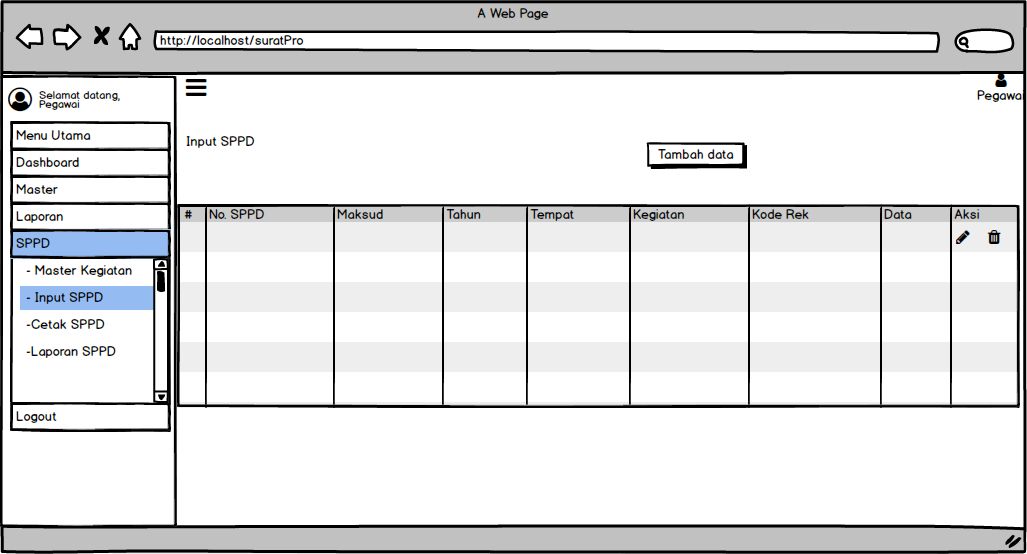
\includegraphics [height= 7cm, width=11cm]{konten/gambar/WireFrameSistemSurat/Pegawai/InputSPPD.png}
			\caption{Halaman Input SPPD Pegawai}
			\label{HalamanHalamanInputSPPDPegawai}
		\end{figure}
		
		\item Laporan Cetak SPPD 
		
		Laporan Cetak SPPD dapat dilihat pada \pic~\ref{HalamanCetakSPPDPegawai}
		
		\begin{figure}
			\centering
			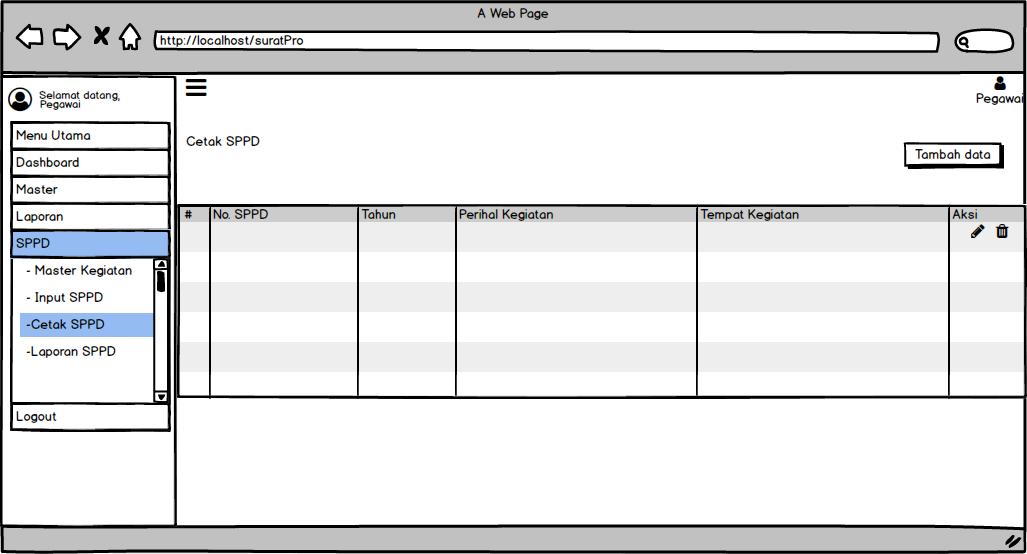
\includegraphics [height= 7cm, width=11cm]{konten/gambar/WireFrameSistemSurat/Pegawai/CetakSPPD.png}
			\caption{Halaman Cetak SPPD Pegawai}
			\label{HalamanCetakSPPDPegawai}
		\end{figure}
		
		\item Laporan SPPD 
		
		Halaman Laporan SPPD  dapat dilihat pada \pic~\ref{HalamanLaporanSPPDPegawai}
		
		\begin{figure}
			\centering
			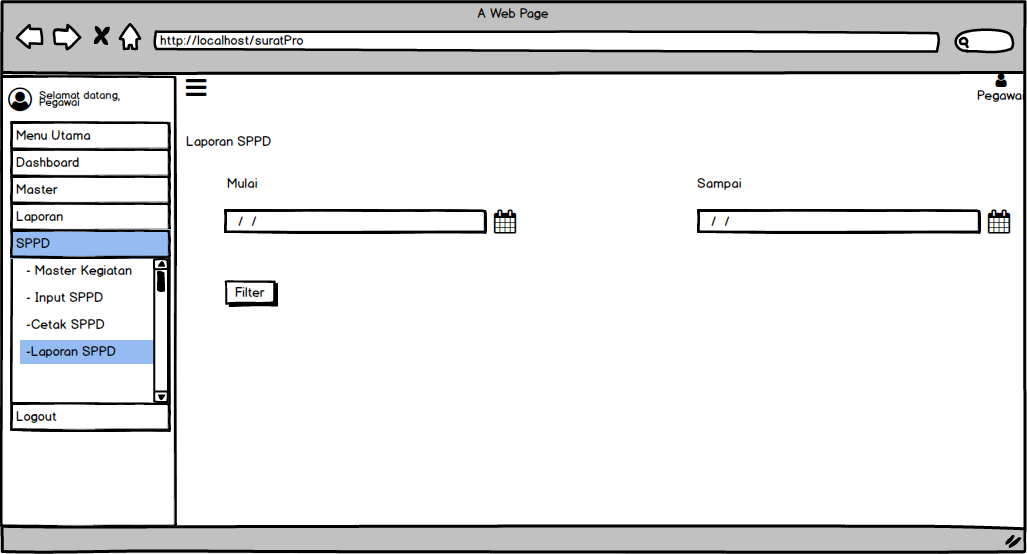
\includegraphics [height= 7cm, width=11cm]{konten/gambar/WireFrameSistemSurat/Pegawai/LaporanSPPD.png}
			\caption{Halaman Laporan SPPD Pegawai}
			\label{HalamanLaporanSPPDPegawai}
		\end{figure}
	\end{enumerate}
\end{enumerate}



\ifthenelse{\equal{\tipeta}{TUGAS AKHIR}}{
  %-----------------------------------------------------------------------------------------------%
%
% Maret 2019
% Template Latex untuk Tugas Akhir Program Studi Sistem informasi ini
% dikembangkan oleh Inggih Permana (inggihjava@gmail.com)
%
% Template ini dikembangkan dari template yang dibuat oleh Andreas Febrian (Fasilkom UI 2003).
%
% Orang yang cerdas adalah orang yang paling banyak mengingat kematian.
%
%-----------------------------------------------------------------------------------------------%

%-----------------------------------------------------------------------------%
\chapter{\babLima}
%-----------------------------------------------------------------------------%

%-----------------------------------------------------------------------------%
\section{Hasil Implementasi}
%-----------------------------------------------------------------------------%
Setelah tahapan dari analisa serta perancangan selesai dilaksanakan maka dilanjutkan ke tahapan dari implementasi dan pengujian. 
Adapun tahapan ini dilakukan pengujian terhadap fitur-fitur yang tersedia pada aplikasi, selanjutnya dilakukan pengamatan dari hasil pengujian tersebut sehingga diketahui fitur-fitur yang masih memiliki kekurangan untuk diambil kesimpulan. Pengujian aplikasi ini menggunakan perangkat PC atau Laptop


\subsection{Lingkungan Implementasi}

Tahap Implmentasi dan pengujian pada sistem surat ini di lakukan terhadap perangkat keras dan perangkat lunak sebagai berikut :
\begin{enumerate}
	\item \textbf{Lingkungan Perangkat lunak}.
	
	Perangkat keras yang digunakan dalam implementasi sistem surat adalah sebagai berikut :
	
	\begin{enumerate}
		\item \textit{Operating System} : Windows 10.
		\item  Bahasa Pemrograman: \textit{CodeIgniter}, dan SQL.
		\item \textit{Web Browser}: Mozilla Firefox dan Google Chroom.
		\item Tools Pengembangan: \textit{Vscode Text Editor}.
		\item \textit{Server}: \textit{XAMPP}.
		\item Pemodelan UML: \textit{Microsoft Visio 2019}.
		\item \textit{Desaign Tools} : Balsamiq Mockup
	\end{enumerate}
	
	\item \textbf{Lingkungan Perangkat Keras}
	\begin{enumerate}
		\item \textit{Processor} : Intel(R) Core(TM) i5-8250u CPU @ 1.6GHz.
		\item \textit{RAM} : 8GB
		\item \textit{SSD} : 256GB
	\end{enumerate}
\end{enumerate}

%-----------------------------------------------------------------------------%
\subsection{Hasil Implementasi}
%-----------------------------------------------------------------------------%
Hasil Implementasi yang dilakukan akan ditampilkan pada sub-bab ini. berikut adalah tampilan awal dari sistem surat  \pic~\ref{loginpage} :
\begin{figure}
	\centering
	\includegraphics[height= 7cm, width=11cm]{konten/gambar/UISistemSurat/0.0.LoginPage.png}
	\caption{Tampilan Halaman \textit{Login}}
	\label{loginpage}
\end{figure}

dan berikut merupakan tampilan halaman sistem sesuai \textit{role} akses masing - masing :

\begin{enumerate}
	\item \textbf{Admin}
	
	berikut adalah tampilan dari sisi admin
	
	\begin{enumerate}
		\item Dashboard
		
		Berikut adalah tampilan untuk melihat Dashboard dapat dilihat pada \pic~\ref{HalamanDashboard}
		
		\begin{figure}
			\centering
			\includegraphics [height= 7cm, width=11cm]{konten/gambar/UISistemSurat/Admin/0.1.Dashboard.png}
			\caption{Halaman Dashboard}
			\label{HalamanDashboard}
		\end{figure}
		
		\item Edit Profil Admin
		
		Berikut adalah tampilan untuk mengakses Halaman Edit Profil Admin dapat dilihat pada \pic~\ref{HalamanEditProfilAdmin}
		
		\begin{figure}
			\centering
			\includegraphics [height= 7cm, width=11cm]{konten/gambar/UISistemSurat/Admin/1.1.DetailProfile.png}
			\caption{Halaman Edit Profil}
			\label{HalamanEditProfilAdmin}
		\end{figure}
		
		\item Lihat Data Golongan Pegawai
		
		Berikut adalah tampilan untuk mengakses Halaman Data Golongan Pegawai dapat dilihat pada \pic~\ref{LihatDataGolonganPegawai}
		
		\begin{figure}
			\centering
			\includegraphics [height= 7cm, width=11cm]{konten/gambar/UISistemSurat/Admin/2.LihatDataGolonganPegawai.png}
			\caption{Lihat Data Golongan Pegawai}
			\label{LihatDataGolonganPegawai}
		\end{figure}
		
		\item Input Data Golongan Pegawai
		
		Berikut adalah tampilan untuk mengakses Halaman Menginput Data Golongan Pegawai dapat dilihat pada  \pic~\ref{InputDataGolonganPegawai}
		
		\begin{figure}
			\centering
			\includegraphics [height= 7cm, width=11cm]{konten/gambar/UISistemSurat/Admin/3.InputDataGolonganPegawai.png}
			\caption{Input Data Golongan Pegawai}
			\label{InputDataGolonganPegawai}
		\end{figure}
		
		\item Lihat Master Jabatan Pegawai
		
		Berikut adalah tampilan untuk mengakses Halaman Melihat Master Jabatan Pegawai dapat dilihat pada \pic~\ref{lihatMasterJabatanPegawai}
		
		\begin{figure}
			\centering
			\includegraphics [height= 7cm, width=11cm]{konten/gambar/UISistemSurat/Admin/4.lihatMasterJabatanPegawai.png}
			\caption{Lihat Master Jabatan Pegawai}
			\label{lihatMasterJabatanPegawai}
		\end{figure}
		
		\item Tambah Data Jabatan Pegawai
		
		Berikut adalah tampilan untuk mengakses Menambah Data Jabatan Pegawai dapat dilihat pada \pic~\ref{TambahDataJabatanPegawai}
		
		\begin{figure}
			\centering
			\includegraphics [height= 7cm, width=11cm]{konten/gambar/UISistemSurat/Admin/5.TambahDataJabatanPegawai.png}
			\caption{Tambah Data Jabatan Pegawai}
			\label{TambahDataJabatanPegawai}
		\end{figure}	
		
		\item Tambah Data Pegawai
		
		Berikut adalah tampilan Menambah data pegawai dapat dilihat pada \pic~\ref{TambahDataPegawai}
		
		\begin{figure}
			\centering
			\includegraphics [height= 7cm, width=11cm]{konten/gambar/UISistemSurat/Admin/6.TambahDataPegawai.png}
			\caption{Tambah Data Pegawai}
			\label{TambahDataPegawai}
		\end{figure}
		
		\item Lihat Struktur Organisasi
		
		Berikut adalah tampilan Melihat Struktur Organisasi dapat dilihat pada \pic~\ref{LihatStrukturOrganisasi}
		
		\begin{figure}
			\centering
			\includegraphics [height= 7cm, width=11cm]{konten/gambar/UISistemSurat/Admin/7.LihatStrukturOrganisasi.png}
			\caption{Lihat Struktur Organisasi}
			\label{LihatStrukturOrganisasi}
		\end{figure}
		
		\item Lihat Kategori Surat
		
		Berikut adalah tampilan Melihat Kategori Surat dapat dilihat pada \pic~\ref{LihatKategoriSurat}
		
		\begin{figure}
			\centering
			\includegraphics [height= 7cm, width=11cm]{konten/gambar/UISistemSurat/Admin/8.LihatKategoriSurat.png}
			\caption{Lihat Kategori Surat}
			\label{LihatKategoriSurat}
		\end{figure}
		
		\item Tambah Kategori Surat
		
		Berikut adalah tampilan Menambah Kategori Surat dapat dilihat pada \pic~\ref{TambahKategoriSurat}
		
		\begin{figure}
			\centering
			\includegraphics [height= 7cm, width=11cm]{konten/gambar/UISistemSurat/Admin/9.TambahKategoriSurat.png}
			\caption{Tambah Kategori Surat}
			\label{TambahKategoriSurat}
		\end{figure}
		
		\item Lihat Master Pengirim Surat
		
		Berikut adalah tampilan Melihat Master Pengirim Surat dapat dilihat pada \pic~\ref{LihatMasterPengirimSurat}
		
		\begin{figure}
			\centering
			\includegraphics [height= 7cm, width=11cm]{konten/gambar/UISistemSurat/Admin/10.LihatMasterPengirimSurat.png}
			\caption{Lihat Master Pengirim Surat}
			\label{LihatMasterPengirimSurat}
		\end{figure}
		
		\item Tambah Data Pengirim Surat
		
		Berikut adalah tampilan Tambah Data Pengirim Surat dapat dilihat pada \pic~\ref{TambahDataPengirimSurat}
		
		\begin{figure}
			\centering
			\includegraphics [height= 7cm, width=11cm]{konten/gambar/UISistemSurat/Admin/11.TambahDataPengirimSurat.png}
			\caption{Tambah Data Pengirim Surat}
			\label{TambahDataPengirimSurat}
		\end{figure}
		
		\item Lihat Tujuan Surat Keluar
		
		Berikut adalah tampilan Lihat Tujuan Surat Keluar dapat dilihat pada \pic~\ref{LihatTujuanSuratKeluar}
		
		\begin{figure}
			\centering
			\includegraphics [height= 7cm, width=11cm]{konten/gambar/UISistemSurat/Admin/12.LihatTujuanSuratKeluar.png}
			\caption{Lihat Tujuan Surat Keluar}
			\label{LihatTujuanSuratKeluar}
		\end{figure}
		
		\item Tambah Data Tujuan Surat Keluar
		
		Berikut adalah tampilan Tambah Data Tujuan Surat Keluar dapat dilihat pada \pic~\ref{TambahDataTujuanSuratKeluar}
		
		\begin{figure}
			\centering
			\includegraphics [height= 7cm, width=11cm]{konten/gambar/UISistemSurat/Admin/13.TambahDataTujuanSuratKeluar.png}
			\caption{Tambah Data Tujuan Surat Keluar}
			\label{TambahDataTujuanSuratKeluar}
		\end{figure}
		
		\item Lihat Data Surat Masuk
		
		Berikut adalah tampilan Lihat Data Surat Masuk dapat dilihat pada \pic~\ref{LihatDataSuratMasuk}
		
		\begin{figure}
			\centering
			\includegraphics [height= 7cm, width=11cm]{konten/gambar/UISistemSurat/Admin/14.LihatDataSuratMasuk.png}
			\caption{Lihat Data Surat Masuk}
			\label{LihatDataSuratMasuk}
		\end{figure}
		
		\item Lihat Data Surat Keluar
		
		Berikut adalah tampilan Lihat Data Surat Keluar dapat dilihat pada \pic~\ref{LihatDataSuratKeluar}
		
		\begin{figure}
			\centering
			\includegraphics [height= 7cm, width=11cm]{konten/gambar/UISistemSurat/Admin/15.LihatDataSuratKeluar.png}
			\caption{Lihat Data Surat Keluar}
			\label{LihatDataSuratKeluar}
		\end{figure}
		
		\item Tambah Data SPPD
		
		Berikut adalah tampilan Tambah Data SPPD dapat dilihat pada \pic~\ref{TambahDataSPPDAdmin}
		
		\begin{figure}
			\centering
			\includegraphics [height= 7cm, width=11cm]{konten/gambar/UISistemSurat/Admin/16.TambahDataSPPD.png}
			\caption{Tambah Data SPPD}
			\label{TambahDataSPPDAdmin}
		\end{figure}
		
		\item Tambah Data SPPD Master
		
		Berikut adalah tampilan Tambah Data SPPD Master dapat dilihat pada \pic~\ref{TambahDataSPPDMasterAdmin}
		
		\begin{figure}
			\centering
			\includegraphics [height= 7cm, width=11cm]{konten/gambar/UISistemSurat/Admin/17.TambahDataSPPDMaster.png}
			\caption{Tambah Data SPPD Master}
			\label{TambahDataSPPDMasterAdmin}
		\end{figure}
		
		\item Lihat Data SPPD
		
		Berikut adalah tampilan Lihat Data SPPD dapat dilihat pada \pic~\ref{LihatDataSPPDAdmin}
		
		\begin{figure}
			\centering
			\includegraphics [height= 7cm, width=11cm]{konten/gambar/UISistemSurat/Admin/18.LihatDataSPPD.png}
			\caption{Lihat Data SPPD}
			\label{LihatDataSPPDAdmin}
		\end{figure}
		
		\item Cetak SPPD
		
		Berikut adalah tampilan Cetak SPPD dapat dilihat pada \pic~\ref{CetakSPPDAdmin}
		
		\begin{figure}
			\centering
			\includegraphics [height= 7cm, width=11cm]{konten/gambar/UISistemSurat/Admin/20.CetakSPPD.png}
			\caption{Cetak SPPD}
			\label{CetakSPPDAdmin}
		\end{figure}
		
		\item Rekap Data SPPD
		
		Berikut adalah tampilan Rekap Data SPPD dapat dilihat pada \pic~\ref{RekapDataSPPDAdmin}
		
		\begin{figure}
			\centering
			\includegraphics [height= 7cm, width=11cm]{konten/gambar/UISistemSurat/Admin/21.RekapDataSPPD.png}
			\caption{RekapDataSPPD}
			\label{RekapDataSPPDAdmin}
		\end{figure}	
	\end{enumerate}
	
	\item \textbf{Kepala Dinas}
	
	\begin{enumerate}
		\item Dashboard
		
		Berikut adalah tampilan Dashboard Kepala Dinas dapat dilihat pada \pic~\ref{DashboardKadis}
		
		\begin{figure}
			\centering
			\includegraphics [height= 7cm, width=11cm]{konten/gambar/UISistemSurat/Kadis/0.1.Dashboard.png}
			\caption{Dashboard Kadis}
			\label{DashboardKadis}
		\end{figure}
		
		\item Notifikasi Disposisi
		
		Berikut adalah tampilan Notifikasi Disposisi dapat dilihat pada \pic~\ref{DashboardKadis}
		
		\begin{figure}
			\centering
			\includegraphics [height= 7cm, width=11cm]{konten/gambar/UISistemSurat/Kadis/0.2.notifikasiDisposisi.png}
			\caption{Notifikasi Disposisi}
			\label{notifikasiDisposisi}
		\end{figure}
		
		\item Halaman Profile
		
		Berikut adalah tampilan Halaman Profile Kadis dapat dilihat pada \pic~\ref{HalamanProfileKadis}
		
		\begin{figure}
			\centering
			\includegraphics [height= 7cm, width=11cm]{konten/gambar/UISistemSurat/Kadis/0.3.HalamanProfile.png}
			\caption{Halaman Profile Kadis}
			\label{HalamanProfileKadis}
		\end{figure}
		
		\item Lihat Master Agenda
		
		Berikut adalah tampilan Lihat Master Agenda Kadis dapat dilihat pada \pic~\ref{LihatMasterAgendaKadis}
		
		\begin{figure}
			\centering
			\includegraphics [height= 7cm, width=11cm]{konten/gambar/UISistemSurat/Kadis/0.4.LihatMasterAgenda.png}
			\caption{Lihat Master Agenda Kadis}
			\label{LihatMasterAgendaKadis}
		\end{figure}
		
		\item Lihat Master Agenda Bulanan
		
		Berikut adalah tampilan Lihat Master Agenda Bulanan Kadis dapat dilihat pada \pic~\ref{LihatMasterAgendaBulananKadis}
		
		\begin{figure}
			\centering
			\includegraphics [height= 7cm, width=11cm]{konten/gambar/UISistemSurat/Kadis/0.5.LihatMasterAgendaBulanan.png}
			\caption{Lihat Master Agenda Bulanan Kadis}
			\label{LihatMasterAgendaBulananKadis}
		\end{figure}
		
		\item Lihat Master Agenda Mingguan
		
		Berikut adalah tampilan Lihat Master Agenda Mingguan Kadis dapat dilihat pada \pic~\ref{LihatMasterAgendaMingguanKadis}
		
		\begin{figure}
			\centering
			\includegraphics [height= 7cm, width=11cm]{konten/gambar/UISistemSurat/Kadis/0.6.LihatMasterAgendaMingguan.png}
			\caption{Lihat Master Agenda Mingguan Kadis}
			\label{LihatMasterAgendaMingguanKadis}
		\end{figure}
		
		\item Lihat Master Agenda Harian
		
		Berikut adalah tampilan Lihat Master Agenda Harian Kadis dapat dilihat pada \pic~\ref{LihatMasterAgendaHarianKadis}
		
		\begin{figure}
			\centering
			\includegraphics [height= 7cm, width=11cm]{konten/gambar/UISistemSurat/Kadis/0.7.LihatMasterAgendaHarian.png}
			\caption{Lihat Master Agenda Harian Kadis}
			\label{LihatMasterAgendaHarianKadis}
		\end{figure}
		
		\item Lihat Data Surat Masuk
		
		Berikut adalah tampilan Lihat Data Surat Masuk Kadis dapat dilihat pada \pic~\ref{LihatDataSuratMasukKadis}
		
		\begin{figure}
			\centering
			\includegraphics [height= 7cm, width=11cm]{konten/gambar/UISistemSurat/Kadis/0.8.LihatDataSuratMasuk.png}
			\caption{Lihat Data Surat Masuk Kadis}
			\label{LihatDataSuratMasukKadis}
		\end{figure}
		
		\item Lihat Laporan Surat Masuk
		
		Berikut adalah tampilan Lihat Laporan Surat Masuk Kadis dapat dilihat pada \pic~\ref{LihatLaporanSuratMasukKadis}
		
		\begin{figure}
			\centering
			\includegraphics [height= 7cm, width=11cm]{konten/gambar/UISistemSurat/Kadis/0.9.LihatLaporanSuratMasuk.png}
			\caption{Lihat Laporan Surat Masuk Kadis}
			\label{LihatLaporanSuratMasukKadis}
		\end{figure}
		
		\item Lihat Laporan Surat Keluar
		
		Berikut adalah tampilan Lihat Laporan Surat Keluar Kadis dapat dilihat pada \pic~\ref{LihatLaporanSuratKeluarKadis}
		
		\begin{figure}
			\centering
			\includegraphics [height= 7cm, width=11cm]{konten/gambar/UISistemSurat/Kadis/0.10.LihatLaporanSuratKeluar.png}
			\caption{Lihat Laporan Surat Keluar Kadis}
			\label{LihatLaporanSuratKeluarKadis}
		\end{figure}
		
		\item Master Data Kegiatan
		
		Berikut adalah tampilan Master Data Kegiatan DPA Kadis dapat dilihat pada \pic~\ref{MasterDataKegiatanDPAKadis}
		
		\begin{figure}
			\centering
			\includegraphics [height= 7cm, width=11cm]{konten/gambar/UISistemSurat/Kadis/0.11.MasterDataKegiatanDPA.png}
			\caption{Master Data Kegiatan DPA Kadis}
			\label{MasterDataKegiatanDPAKadis}
		\end{figure}
		
		\item Lihat Data Master
		
		Berikut adalah tampilan Lihat Data Master DPA Kadis dapat dilihat pada \pic~\ref{LihatDataMasterDPAKadis}
		
		\begin{figure}
			\centering
			\includegraphics [height= 7cm, width=11cm]{konten/gambar/UISistemSurat/Kadis/0.12.LihatDataMasterDPA.png}
			\caption{Lihat Data Master DPA Kadis}
			\label{LihatDataMasterDPAKadis}
		\end{figure}
		
		\item Tambah Master Kegiatan
		
		Berikut adalah tampilan Tambah Master Kegiatan DPA Kadis dapat dilihat pada \pic~\ref{TambahMasterKegiatanDPAKadis}
		
		\begin{figure}
			\centering
			\includegraphics [height= 7cm, width=11cm]{konten/gambar/UISistemSurat/Kadis/0.13.TambahMasterKegiatanDPA.png}
			\caption{Tambah Master Kegiatan DPA Kadis}
			\label{TambahMasterKegiatanDPAKadis}
		\end{figure}
		
		\item Lihat Data SPPD
		
		Berikut adalah tampilan Lihat Data SPPD Kadis dapat dilihat pada \pic~\ref{LihatDataSPPDKadis}
		
		\begin{figure}
			\centering
			\includegraphics [height= 7cm, width=11cm]{konten/gambar/UISistemSurat/Kadis/0.14.LihatDataSPPD.png}
			\caption{Lihat Data SPPD Kadis}
			\label{LihatDataSPPDKadis}
		\end{figure}
		
		\item Input Data SPPD
		
		Berikut adalah tampilan Input Data SPPD Kadis dapat dilihat pada \pic~\ref{InputDataSPPDKadis}
		
		\begin{figure}
			\centering
			\includegraphics [height= 7cm, width=11cm]{konten/gambar/UISistemSurat/Kadis/0.15.InputDataSPPD.png}
			\caption{Input Data SPPD Kadis}
			\label{InputDataSPPDKadis}
		\end{figure}
		
		\item Cetak SPPD
		
		Berikut adalah tampilan Cetak SPPD Kadis dapat dilihat pada \pic~\ref{CetakSPPDKadis}
		
		\begin{figure}
			\centering
			\includegraphics [height= 7cm, width=11cm]{konten/gambar/UISistemSurat/Kadis/0.16.CetakSPPD.png}
			\caption{Cetak SPPD Kadis}
			\label{CetakSPPDKadis}
		\end{figure}
		
		\item Rekap SPPD
		
		Berikut adalah tampilan Rekap SPPD Kadis dapat dilihat pada \pic~\ref{RekapSPPDKadis}
		
		\begin{figure}
			\centering
			\includegraphics [height= 7cm, width=11cm]{konten/gambar/UISistemSurat/Kadis/0.17.RekapSPPD.png}
			\caption{Rekap SPPD Kadis}
			\label{RekapSPPDKadis}
		\end{figure}
	\end{enumerate}
	
	\item \textbf{Pengagenda}
	
	\begin{enumerate}
		\item Halaman Dashboard
		
		Berikut Adalah Halaman Dashboard yang dapat dilihat pada \pic~\ref{Dashboardpengagenda}
		
		\begin{figure}
			\centering
			\includegraphics [height= 7cm, width=11cm]{konten/gambar/UISistemSurat/Pengagenda/0.1.Dashboard.png}
			\caption{Dashboard Pengagenda}
			\label{Dashboardpengagenda}
		\end{figure}
		
		\item Detail Profile Pengagenda
		
		Berikut Adalah Detail Profile Pengagenda yang dapat dilihat pada \pic~\ref{DetailProfilePengagenda}
		
		\begin{figure}
			\centering
			\includegraphics [height= 7cm, width=11cm]{konten/gambar/UISistemSurat/Pengagenda/0.2.DetailProfile.png}
			\caption{Detail Profile Pengagenda}
			\label{DetailProfilePengagenda}
		\end{figure}
		
		\item Lihat Master Agenda Pengagenda
		
		Berikut Adalah Lihat Master Agenda Pengagenda yang dapat dilihat pada \pic~\ref{LihatMasterAgendaPengagenda}
		
		\begin{figure}
			\centering
			\includegraphics [height= 7cm, width=11cm]{konten/gambar/UISistemSurat/Pengagenda/0.3.LihatMasterAgenda.png}
			\caption{Lihat Master Agenda Pengagenda}
			\label{LihatMasterAgendaPengagenda}
		\end{figure}
		
		\item Lihat Master Agenda Bulanan Pengagenda
		
		Berikut Adalah Lihat Master Agenda Bulanan Pengagenda yang dapat dilihat pada \pic~\ref{LihatMasterAgendaBulananPengagenda}
		
		\begin{figure}
			\centering
			\includegraphics [height= 7cm, width=11cm]{konten/gambar/UISistemSurat/Pengagenda/0.4.LihatMasterAgendaBulanan.png}
			\caption{Lihat Master Agenda Bulanan Pengagenda}
			\label{LihatMasterAgendaBulananPengagenda}
		\end{figure}
		
		\item Lihat Master Agenda Mingguan Pengagenda
		
		Berikut Adalah Lihat Master Agenda Mingguan Pengagenda yang dapat dilihat pada \pic~\ref{LihatMasterAgendaMingguanPengagenda}
		
		\begin{figure}
			\centering
			\includegraphics [height= 7cm, width=11cm]{konten/gambar/UISistemSurat/Pengagenda/0.5.LihatMasterAgendaMingguan.png}
			\caption{Lihat Master Agenda Mingguan Pengagenda}
			\label{LihatMasterAgendaMingguanPengagenda}
		\end{figure}
		
		
		\item Lihat Master Agenda Harian Pengagenda
		
		Berikut Adalah Lihat Master Agenda Harian Pengagenda yang dapat dilihat pada \pic~\ref{LihatMasterAgendaHarianPengagenda}
		
		\begin{figure}
			\centering
			\includegraphics [height= 7cm, width=11cm]{konten/gambar/UISistemSurat/Pengagenda/0.6.LihatMasterAgendaHarian.png}
			\caption{Lihat Master Agenda Harian Pengagenda}
			\label{LihatMasterAgendaHarianPengagenda}
		\end{figure}
		
		
		\item Tambah Agenda Pengagenda
		
		Berikut Adalah Tambah Agenda Pengagenda yang dapat dilihat pada \pic~\ref{TambahAgendaPengagenda}
		
		\begin{figure}
			\centering
			\includegraphics [height= 7cm, width=11cm]{konten/gambar/UISistemSurat/Pengagenda/0.7.TambahAgenda.png}
			\caption{Tambah Agenda Pengagenda}
			\label{TambahAgendaPengagenda}
		\end{figure}
		
		
		\item Tambah Data Surat Masuk Pengagenda
		
		Berikut Adalah Tambah Data Surat Masuk Pengagenda yang dapat dilihat pada \pic~\ref{TambahDataSuratMasukPengagenda}
		
		\begin{figure}
			\centering
			\includegraphics [height= 7cm, width=11cm]{konten/gambar/UISistemSurat/Pengagenda/0.9.TambahDataSuratMasuk.png}
			\caption{Tambah Data Surat Masuk Pengagenda}
			\label{TambahDataSuratMasukPengagenda}
		\end{figure}
		
		
		\item Lihat Data Surat Masuk Pengagenda
		
		Berikut Adalah Lihat Data Surat Masuk Pengagenda yang dapat dilihat pada \pic~\ref{LihatDataSuratMasukPengagenda}
		
		\begin{figure}
			\centering
			\includegraphics [height= 7cm, width=11cm]{konten/gambar/UISistemSurat/Pengagenda/0.10.LihatDataSuratMasuk.png}
			\caption{Lihat Data Surat Masuk Pengagenda}
			\label{LihatDataSuratMasukPengagenda}
		\end{figure}
		
		
		\item Lihat Data Surat Keluar Pengagenda
		
		Berikut Adalah Lihat Data Surat Keluar Pengagenda yang dapat dilihat pada \pic~\ref{LihatDataSuratKeluarPengagenda}
		
		\begin{figure}
			\centering
			\includegraphics [height= 7cm, width=11cm]{konten/gambar/UISistemSurat/Pengagenda/0.11.LihatDataSuratKeluar.png}
			\caption{Lihat Data Surat Keluar Pengagenda}
			\label{LihatDataSuratKeluarPengagenda}
		\end{figure}
		
		
		\item Data Master DPA Pengagenda
		
		Berikut Adalah Data Master DPA Pengagenda yang dapat dilihat pada \pic~\ref{DataMasterDPAPengagenda}
		
		\begin{figure}
			\centering
			\includegraphics [height= 7cm, width=11cm]{konten/gambar/UISistemSurat/Pengagenda/0.12.DataMasterDPA.png}
			\caption{Data Master DPA Pengagenda}
			\label{DataMasterDPAPengagenda}
		\end{figure}
		
		
		\item Input Master DPA Pengagenda
		
		Berikut Adalah Input Master DPA Pengagenda yang dapat dilihat pada \pic~\ref{InputMasterDPAPengagenda}
		
		\begin{figure}
			\centering
			\includegraphics [height= 7cm, width=11cm]{konten/gambar/UISistemSurat/Pengagenda/0.13.InputMasterDPA.png}
			\caption{Input Master DPA Pengagenda}
			\label{InputMasterDPAPengagenda}
		\end{figure}
		
		
		\item Lihat Data SPPD Pengagenda
		
		Berikut Adalah Lihat Data SPPD Pengagenda yang dapat dilihat pada \pic~\ref{LihatDataSPPDPengagenda}
		
		\begin{figure}
			\centering
			\includegraphics [height= 7cm, width=11cm]{konten/gambar/UISistemSurat/Pengagenda/0.14.LihatDataSPPD.png}
			\caption{Lihat Data SPPD Pengagenda}
			\label{LihatDataSPPDPengagenda}
		\end{figure}
		
		
		\item Tambah Data SPPD Pengagenda
		
		Berikut Adalah Tambah Data SPPD Pengagenda yang dapat dilihat pada \pic~\ref{TambahDataSPPDPengagenda}
		
		\begin{figure}
			\centering
			\includegraphics [height= 7cm, width=11cm]{konten/gambar/UISistemSurat/Pengagenda/0.15.TambahDataSPPD.png}
			\caption{Tambah Data SPPD Pengagenda}
			\label{TambahDataSPPDPengagenda}
		\end{figure}
		
		
		\item Cetak Data SPPD Pengagenda
		
		Berikut Adalah Cetak Data SPPD Pengagenda yang dapat dilihat pada \pic~\ref{CetakDataSPPDPengagenda}
		
		\begin{figure}
			\centering
			\includegraphics [height= 7cm, width=11cm]{konten/gambar/UISistemSurat/Pengagenda/0.16.CetakDataSPPD.png}
			\caption{Cetak Data SPPD Pengagenda}
			\label{CetakDataSPPDPengagenda}
		\end{figure}
		
		
		\item Rekap Data SPPD 
		
		Berikut Adalah Rekap Data SPPD yang dapat dilihat pada \pic~\ref{RekapDataSPPD}
		
		\begin{figure}
			\centering
			\includegraphics [height= 7cm, width=11cm]{konten/gambar/UISistemSurat/Pengagenda/0.17.RekapDataSPPD.png}
			\caption{Rekap Data SPPD}
			\label{RekapDataSPPD}
		\end{figure}
		
	\end{enumerate}
	
	\item \textbf{Pegawai}
	
	\begin{enumerate}
		\item Halaman Dashboard
		
		Berikut Adalah Halaman Dashboard yang dapat dilihat pada \pic~\ref{DashboardPegawai}
		
		\begin{figure}
			\centering
			\includegraphics [height= 7cm, width=11cm]{konten/gambar/UISistemSurat/Pegawai/0.1.Dashboard.png}
			\caption{DashboardPegawai}
			\label{DashboardPegawai}
		\end{figure}
		
		\item Notifikasi Disposisi Pegawai
		
		Berikut Adalah NotifikasiDisposisiPegawai yang dapat dilihat pada \pic~\ref{NotifikasiDisposisiPegawai}
		
		\begin{figure}
			\centering
			\includegraphics [height= 7cm, width=11cm]{konten/gambar/UISistemSurat/Pegawai/0.2NotifikasiDisposisi.png}
			\caption{NotifikasiDisposisiPegawai}
			\label{NotifikasiDisposisiPegawai}
		\end{figure}
		
		\item Detail Profile Pegawai
		
		Berikut Adalah Detail Profile Pegawai yang dapat dilihat pada \pic~\ref{DetailProfilePegawai}
		
		\begin{figure}
			\centering
			\includegraphics [height= 7cm, width=11cm]{konten/gambar/UISistemSurat/Pegawai/0.3.DetailProfile.png}
			\caption{Detail Profile Pegawai}
			\label{DetailProfilePegawai}
		\end{figure}
		
		
		\item Data Surat Masuk Pegawai
		
		Berikut Adalah Data Surat Masuk Pegawai yang dapat dilihat pada \pic~\ref{DataSuratMasukPegawai}
		
		\begin{figure}
			\centering
			\includegraphics [height= 7cm, width=11cm]{konten/gambar/UISistemSurat/Pegawai/0.4.DataSuratMasuk.png}
			\caption{Data Surat Masuk Pegawai}
			\label{DataSuratMasukPegawai}
		\end{figure}
		
		\item Laporan Surat Masuk Pegawai
		
		Berikut Adalah Laporan Surat Masuk Pegawai yang dapat dilihat pada \pic~\ref{LaporanSuratMasukPegawai}
		
		\begin{figure}
			\centering
			\includegraphics [height= 7cm, width=11cm]{konten/gambar/UISistemSurat/Pegawai/0.5.LaporanSuratMasuk.png}
			\caption{Laporan Surat Masuk Pegawai}
			\label{LaporanSuratMasukPegawai}
		\end{figure}
		
		\item Laporan Surat Keluar Pegawai
		
		Berikut Adalah Laporan Surat Keluar Pegawai yang dapat dilihat pada \pic~\ref{LaporanSuratKeluarPegawai}
		
		\begin{figure}
			\centering
			\includegraphics [height= 7cm, width=11cm]{konten/gambar/UISistemSurat/Pegawai/0.6.LaporanSuratKeluar.png}
			\caption{Laporan Surat Keluar Pegawai}
			\label{LaporanSuratKeluarPegawai}
		\end{figure}
		
		\item Lihat Data Master Kegiatan DPA Pegawai
		
		Berikut Adalah Lihat Data Master Kegiatan DPA Pegawai yang dapat dilihat pada \pic~\ref{LihatDataMasterKegiatanDPAPegawai}
		
		\begin{figure}
			\centering
			\includegraphics [height= 7cm, width=11cm]{konten/gambar/UISistemSurat/Pegawai/0.7.LihatDataMasterKegiatanDPA.png}
			\caption{Lihat Data Master Kegiatan DPA Pegawai}
			\label{LihatDataMasterKegiatanDPAPegawai}
		\end{figure}
		
		\item Tambah Data Kegiatan DPA Pegawai
		
		Berikut Adalah Tambah Data Kegiatan DPA Pegawai yang dapat dilihat pada \pic~\ref{TambahDataKegiatanDPAPegawai}
		
		\begin{figure}
			\centering
			\includegraphics [height= 7cm, width=11cm]{konten/gambar/UISistemSurat/Pegawai/0.8.TambahDataKegiatanDPA.png}
			\caption{Tambah Data Kegiatan DPA Pegawai}
			\label{TambahDataKegiatanDPAPegawai}
		\end{figure}
		
		\item Lihat Data SPPD Pegawai
		
		Berikut Adalah Lihat Data SPPD Pegawai yang dapat dilihat pada \pic~\ref{LihatDataSPPDPegawai}
		
		\begin{figure}
			\centering
			\includegraphics [height= 7cm, width=11cm]{konten/gambar/UISistemSurat/Pegawai/0.9.LihatDataSPPD.png}
			\caption{Lihat Data SPPD Pegawai}
			\label{LihatDataSPPDPegawai}
		\end{figure}
		
		
		\item Tambah Data SPPD Pegawai
		
		Berikut Adalah Tambah Data SPPD Pegawai yang dapat dilihat pada \pic~\ref{TambahDataSPPDPegawai}
		
		\begin{figure}
			\centering
			\includegraphics [height= 7cm, width=11cm]{konten/gambar/UISistemSurat/Pegawai/0.10.TambahDataSPPD.png}
			\caption{Tambah Data SPPD Pegawai}
			\label{TambahDataSPPDPegawai}
		\end{figure}
		
		
		\item Cetak SPPD Pegawai
		
		Berikut Adalah Cetak SPPD Pegawai yang dapat dilihat pada \pic~\ref{CetakSPPDPegawai}
		
		\begin{figure}
			\centering
			\includegraphics [height= 7cm, width=11cm]{konten/gambar/UISistemSurat/Pegawai/0.11.CetakSPPD.png}
			\caption{Cetak SPPD Pegawai}
			\label{CetakSPPDPegawai}
		\end{figure}
		
		
		\item Rekap SPPD Pegawai
		
		Berikut Adalah Rekap SPPD Pegawai yang dapat dilihat pada \pic~\ref{RekapSPPDPegawai}
		
		\begin{figure}
			\centering
			\includegraphics [height= 7cm, width=11cm]{konten/gambar/UISistemSurat/Pegawai/0.12.RekapSPPD.png}
			\caption{Rekap SPPD Pegawai}
			\label{RekapSPPDPegawai}
		\end{figure}
	\end{enumerate}
	
\end{enumerate}


\section{Pengujian Sistem}
Setelah tahapan dari analisa serta perancangan selesai dilaksanakan maka dilanjutkan ke
tahapan dari implementasi dan pengujian. Adapun tahapan ini dilakukan pengujian terhadap fitur-
fitur yang tersedia pada aplikasi, selanjutnya dilakukan pengamatan dari hasil pengujian tersebut
sehingga diketahui fitur-fitur yang masih memiliki kekurangan untuk diambil kesimpulan. Pengujian
aplikasi ini menggunakan perangkat PC dan Laptop.

\subsection {\textit{Blackbox Testing}}.


Pengujian yang dilakukan terhadap aplikasi adalah menggunakan metode \textit{blackbox testing}. Aplikasi ini dari sisi spesifikasi secara fungsional tanpa menguji desain serta kode program di dalamnya. Tujuan dari pengujian ini ditujukan untukmengetahui fungsi-fungsi, masukan serta keluaran dari aplikasi sesuai dengan spesifikasi yang diperlukan.
\begin{enumerate}
	\item \textit{Blackbox Testing} Bagian Admin
	
	Berikut adalah tabel \textit{Blackbox} pada \textit{role} Admin. Dapat dilihat pada \tab~\ref{blackboxtesting}
	 {\fontsize{10pt}{12pt}\selectfont
	\renewcommand\namaTabel{Hasil pengujian \textit{blackbox testing} Admin}
		
	\begin{longtable}{p{0.5cm} p{4cm} p{4cm} p{0.5cm} p{1cm}}
		\caption{Tabel \textit{Blackbox} Admin}
		\label{blackboxtesting}\\ 
		\hline
		\multicolumn{1}{c}{\multirow{2}{*}{\textbf{No}}} & \multicolumn{1}{c}{\multirow{2}{*}{\textbf{Pengujian}}} & \multicolumn{1}{c}{\multirow{2}{*}{\textbf{Interface yang Diharapkan}}} & \multicolumn{2}{c}{\textbf{Hasil Uji}} \\ \cline{4-5} 
		\multicolumn{1}{c}{} & \multicolumn{1}{c}{} & \multicolumn{1}{c}{} & \multicolumn{1}{c}{\textbf{Berhasil}} & \multicolumn{1}{c}{\textbf{Tidak Berhasil}} \\ \hline
		\endfirsthead
		%
		\multicolumn{5}{c}{\tablename\ \thetable\ \namaTabel \space (Tabel
			lanjutan...)} \\
		\hline
		\multicolumn{1}{c}{\multirow{2}{*}{\textbf{No}}} & \multicolumn{1}{c}{\multirow{2}{*}{\textbf{Pengujian}}} & \multicolumn{1}{c}{\multirow{2}{*}{\textbf{Interface yang Diharapkan}}} & \multicolumn{2}{c}{\textbf{Hasil Uji}} \\ \cline{4-5} 
		\multicolumn{1}{c}{} & \multicolumn{1}{c}{} & \multicolumn{1}{c}{} & \multicolumn{1}{c}{\textbf{Berhasil}} & \multicolumn{1}{c}{\textbf{Tidak Berhasil}} \\ \hline
		\endhead
		%
		1 & \textit{Admin} tidak mengisi \textit{username} dan \textit{password} & Tampil notifikasi \textit{username} atau \textit{password} tidak boleh kosong & \checkmark & -\\
		2 & \textit{Username} atau \textit{password} yang dimasukkan salah & Tampil notifikasi \textit{username} atau \textit{password} yang dimasukkan salah & \checkmark & -\\
		3 & \textit{Username} dan \textit{password} yang di masukkan benar & Masuk ke halaman \textit{dashboard Administrator} & \checkmark & -\\
		4 & \textit{Admin} Mengklik menu Edit Profil  & Data edit profil ditampilkan & \checkmark & -\\
		5 & \textit{Admin} Mengubah Data pada  menu Edit Profil  & Data edit profil disimpan ke \textit{Database} & \checkmark & -\\
		6 & \textit{Admin} Mengklik Data Golongan Pegawai & Data Golongan Pegawai ditampilkan & \checkmark & -\\
		7 & \textit{Admin} Menambahkan Data Golongan Pegawai & Data Golongan Pegawai disimpan ke \textit{Database}  & \checkmark & -\\
		8 & \textit{Admin} mengisi Data Golongan Pegawai & Data jadwal berhasil ditambahkan & \checkmark & -\\
		9 & \textit{Admin} mengklik Lihat Master Jabatan Pegawai & Data Lihat Master Jabatan Pegawai ditampilkan & \checkmark & -\\
		10 & \textit{Admin} Menambahkan Jabatan Pegawai & Data Jabatan Pegawai disimpan ke \textit{Database}  & \checkmark & -\\
		11 & \textit{Admin} Mengklik Data Pegawai & Data Pegawai ditampilkan  & \checkmark & -\\
		12 & \textit{Admin} Menambahkan Data Pegawai & Data Pegawai berhasil disimpan ke \textit{database}  & \checkmark & -\\
		13 & \textit{Admin} Mengklik Struktur Organisasi & Data Struktur Organisasi Berhasil ditampilkan  & \checkmark & -\\
		14 & \textit{Admin} Mengklik Lihat Kategori Surat & Lihat Kategori Surat Berhasil ditampilkan  & \checkmark & -\\
		15 & \textit{Admin} Mengklik Tambah Kategori Surat & Kategori Surat Berhasil disimpan ke \textit{Database}  & \checkmark & -\\
		16 & \textit{Admin} Mengklik Lihat Master Pengirim Surat & Lihat Master Pengirim Surat Berhasil Ditampilkan  & \checkmark & -\\
		17 & \textit{Admin} Menambahkan Lihat Master Pengirim Surat & Lihat Master Pengirim Surat disimpan ke \textit{Database}  & \checkmark & -\\
		18 & \textit{Admin} Mengklik Tambah Data Pengirim Surat & Tambah Data Pengirim Surat Berhasil Ditampilkan  & \checkmark & -\\
		19 & \textit{Admin} Menambahkan Tambah Data Pengirim Surat & Data Pengirim Surat Berhasil disimpan ke \textit{Database}  & \checkmark & -\\
		20 & \textit{Admin} Mengklik Lihat Tujuan Surat Keluar & Kategori Surat Berhasil Ditampilkan  & \checkmark & -\\
		21 & \textit{Admin} Menambahkan Lihat Tujuan Surat Keluar & Kategori Surat Berhasil disimpan ke \textit{Database}  & \checkmark & -\\
		22 & \textit{Admin} Mengklik Tambah Data Tujuan Surat Keluar & Tambah Data Tujuan Surat Keluar ditampilkan  & \checkmark & -\\
		23 & \textit{Admin} Menambahkan Tambah Data Tujuan Surat Keluar & Tambah Data Tujuan Surat Keluar Berhasil disimpan ke \textit{Database}  & \checkmark & -\\
		24 & \textit{Admin} Mengklik Lihat Data Surat Masuk & Kategori Surat Berhasil Ditampilkan  & \checkmark & -\\
		25 & \textit{Admin} Menambahkan Lihat Data Surat Masuk & Lihat Data Surat Masuk Berhasil disimpan ke \textit{Database}  & \checkmark & -\\
		26 & \textit{Admin} Mengklik Lihat Data Surat Keluar & Lihat Data Surat Keluar Berhasil Ditampilkan  & \checkmark & -\\
		27 & \textit{Admin} Menambahkan Lihat Data Surat Keluar & Lihat Data Surat Keluar Berhasil disimpan ke \textit{Database}  & \checkmark & -\\
		28 & \textit{Admin} Mengklik Tambah Data SPPD & Tambah Data SPPD Berhasil Ditampilkan  & \checkmark & -\\
		29 & \textit{Admin} Menambahkan Tambah Data SPPD & Tambah Data SPPD Berhasil disimpan ke \textit{Database}  & \checkmark & -\\
		30 & \textit{Admin} Mengklik Tambah Data SPPD Master & Tambah Data SPPD Master Berhasil Ditampilkan  & \checkmark & -\\
		31 & \textit{Admin} Menambahkan Tambah Data SPPD Master & Tambah Data SPPD Master Berhasil disimpan ke \textit{Database}  & \checkmark & -\\
		32 & \textit{Admin} Mengklik Lihat Data SPPD & Lihat Data SPPD Berhasil Ditampilkan  & \checkmark & -\\
		33 & \textit{Admin} Menambahkan Lihat Data SPPD & Lihat Data SPPD Berhasil disimpan ke \textit{Database}  & \checkmark & -\\
		34 & \textit{Admin} Mengklik Cetak SPPD & Cetak SPPD Master Berhasil Ditampilkan  & \checkmark & -\\
		35 & \textit{Admin} MMengklik Cetak SPPD & Cetak SPPD Master Berhasil Dicetak  & \checkmark & -\\		
		36 & \textit{Admin} Mengklik Rekap Data SPPD & Rekap Data SPPD Berhasil Ditampilkan  & \checkmark & -\\
		37 & \textit{Admin} Menambahkan Rekap Data SPPD & Rekap Data SPPD Berhasil  & \checkmark & -\\
		38 & \textit{Admin} Mengklik Menu \textit{logout} & \textit{logout} Berhasil  & \checkmark & -\\\hline
		\end{longtable}}
	
	
	
	\item \textit{Blackbox Testing} Bagian Kepala Dinas
	
	Berikut adalah tabel \textit{Blackbox} pada \textit{role} Kepala Dinas. Dapat dilihat pada \tab~\ref{blackboxtesting2}
	{\fontsize{10pt}{12pt}\selectfont
		\renewcommand\namaTabel{Hasil pengujian \textit{blackbox testing} Kepala Dinas}
		
		\begin{longtable}{p{0.5cm} p{4cm} p{5cm} p{0.5cm} p{1cm}}
			\caption{Tabel \textit{Blackbox} Kepala Dinas}
			\label{blackboxtesting2}\\ 
			\hline
			\multicolumn{1}{c}{\multirow{2}{*}{\textbf{No}}} & \multicolumn{1}{c}{\multirow{2}{*}{\textbf{Pengujian}}} & \multicolumn{1}{c}{\multirow{2}{*}{\textbf{Interface yang Diharapkan}}} & \multicolumn{2}{c}{\textbf{Hasil Uji}} \\ \cline{4-5} 
			\multicolumn{1}{c}{} & \multicolumn{1}{c}{} & \multicolumn{1}{c}{} & \multicolumn{1}{c}{\textbf{Berhasil}} & \multicolumn{1}{c}{\textbf{Tidak Berhasil}} \\ \hline
			\endfirsthead
			%
			\multicolumn{5}{c}{\tablename\ \thetable\ \namaTabel \space (Tabel
				lanjutan...)} \\
			\hline
			\multicolumn{1}{c}{\multirow{2}{*}{\textbf{No}}} & \multicolumn{1}{c}{\multirow{2}{*}{\textbf{Pengujian}}} & \multicolumn{1}{c}{\multirow{2}{*}{\textbf{Interface yang Diharapkan}}} & \multicolumn{2}{c}{\textbf{Hasil Uji}} \\ \cline{4-5} 
			\multicolumn{1}{c}{} & \multicolumn{1}{c}{} & \multicolumn{1}{c}{} & \multicolumn{1}{c}{\textbf{Berhasil}} & \multicolumn{1}{c}{\textbf{Tidak Berhasil}} \\ \hline
			\endhead
			%
			1 & Kepala Dinas tidak mengisi \textit{username} dan \textit{password} & Tampil notifikasi \textit{username} atau \textit{password} tidak boleh kosong & \checkmark & -\\
			2 & \textit{Username} atau \textit{password} yang dimasukkan salah & Tampil notifikasi \textit{username} atau \textit{password} yang dimasukkan salah & \checkmark & -\\
			3 & \textit{Username} dan \textit{password} yang di masukkan benar & Masuk ke halaman \textit{dashboard Kepala Dinasistrator} & \checkmark & -\\
			4 & \textit{Username} atau \textit{password} yang dimasukkan salah & Tampil notifikasi \textit{username} atau \textit{password} yang dimasukkan salah & \checkmark & -\\
			5 & \textit{Username} dan \textit{password} yang di masukkan benar & Masuk ke halaman \textit{dashboard Kepala Dinasistrator} & \checkmark & -\\
			6 & Kepala Dinas Mengklik menu Edit Profil  & Data edit profil ditampilkan & \checkmark & -\\
			7 & Kepala Dinas Mengubah Data pada  menu Edit Profil  & Data edit profil disimpan ke \textit{Database} & \checkmark & -\\
			8 & Kepala Dinas Mengklik data disposisi Surat & Menu Disposisi ditampilkan & \checkmark & -\\
			9 & Kepala Dinas Mendisposisikan Surat  & Surat yang didisposisi Tersimpan ke \textit{Database} & \checkmark & -\\
			10 & Kepala Dinas Mengklik Lihat Master Agenda & Lihat Master Agenda ditampilkan & \checkmark & -\\		
			11 & Kepala Dinas mengklik Lihat Master Agenda Bulanan & Data Lihat Master Agenda Bulanan ditampilkan & \checkmark & -\\
			12 & Kepala Dinas Mengklik Lihat Master Agenda Mingguan & Lihat Master Agenda Mingguan ditampilkan  & \checkmark & -\\		
			13 & Kepala Dinas Mengklik Lihat Master Agenda Harian & Data Lihat Master Agenda Harian Berhasil ditampilkan  & \checkmark & -\\
			14 & Kepala Dinas Mengklik Lihat Data Surat Masuk & Lihat Data Surat Masuk Berhasil ditampilkan  & \checkmark & -\\
			15 & Kepala Dinas Mengklik Lihat Laporan  Surat Masuk & Lihat Laporan  Surat Masuk Berhasil Ditampilkan  & \checkmark & -\\
			16 & Kepala Dinas Mengklik Lihat Laporan Surat Keluar & Lihat Laporan Surat Keluar Berhasil Ditampilkan  & \checkmark & -\\
			17 & Kepala Dinas Mengklik Menu Master Data Kegiatan DPA & Menu Master Data Kegiatan DPA Ditampilkan  & \checkmark & -\\
			18 & Kepala Dinas Menambahkan Master Data Kegiatan DPA & Master Data Kegiatan DPA Berhasil disimpan ke \textit{Database}  & \checkmark & -\\
			19 & Kepala Dinas Mengklik Tambah Data SPPD & Tambah Data SPPD Berhasil Ditampilkan  & \checkmark & -\\
			20 & Kepala Dinas Menambahkan Tambah Data SPPD & Tambah Data SPPD Berhasil disimpan ke \textit{Database}  & \checkmark & -\\
			21 & Kepala Dinas Mengklik Tambah Data SPPD Master & Tambah Data SPPD Master Berhasil Ditampilkan  & \checkmark & -\\
			22 & Kepala Dinas Menambahkan Tambah Data SPPD Master & Tambah Data SPPD Master Berhasil disimpan ke \textit{Database}  & \checkmark & -\\
			23 & Kepala Dinas Mengklik Lihat Data SPPD & Lihat Data SPPD Berhasil Ditampilkan  & \checkmark & -\\
			24 & Kepala Dinas Menambahkan Lihat Data SPPD & Lihat Data SPPD Berhasil disimpan ke \textit{Database}  & \checkmark & -\\
			25 & Kepala Dinas Mengklik Cetak SPPD & Cetak SPPD Master Berhasil Ditampilkan  & \checkmark & -\\
			26 & Kepala Dinas MMengklik Cetak SPPD & Cetak SPPD Master Berhasil Dicetak  & \checkmark & -\\		
			27 & Kepala Dinas Mengklik Rekap Data SPPD & Rekap Data SPPD Berhasil Ditampilkan  & \checkmark & -\\
			28 & Kepala Dinas Menambahkan Rekap Data SPPD & Rekap Data SPPD Berhasil  & \checkmark & -\\
			29 & Kepala Dinas Mengklik Menu \textit{logout} & \textit{logout} berhasil  & \checkmark & -\\\hline
			
			\end{longtable}}
	
	\item \textit{Blackbox Testing} Bagian Pengagenda
	
	Berikut adalah tabel \textit{Blackbox} pada \textit{role} Pengagenda. Dapat dilihat pada \tab~\ref{blackboxtesting3}
	{\fontsize{10pt}{12pt}\selectfont
		\renewcommand\namaTabel{Hasil pengujian \textit{blackbox testing} Pengagenda}
		
		\begin{longtable}{p{0.5cm} p{4cm} p{4cm} p{0.5cm} p{1cm}}
			\caption{Tabel \textit{Blackbox} Pengagenda}
			\label{blackboxtesting3}\\ 
			\hline
			\multicolumn{1}{c}{\multirow{2}{*}{\textbf{No}}} & \multicolumn{1}{c}{\multirow{2}{*}{\textbf{Pengujian}}} & \multicolumn{1}{c}{\multirow{2}{*}{\textbf{Interface yang Diharapkan}}} & \multicolumn{2}{c}{\textbf{Hasil Uji}} \\ \cline{4-5} 
			\multicolumn{1}{c}{} & \multicolumn{1}{c}{} & \multicolumn{1}{c}{} & \multicolumn{1}{c}{\textbf{Berhasil}} & \multicolumn{1}{c}{\textbf{Tidak Berhasil}} \\ \hline
			\endfirsthead
			%
			\multicolumn{5}{c}{\tablename\ \thetable\ \namaTabel \space (Tabel
				lanjutan...)} \\
			\hline
			\multicolumn{1}{c}{\multirow{2}{*}{\textbf{No}}} & \multicolumn{1}{c}{\multirow{2}{*}{\textbf{Pengujian}}} & \multicolumn{1}{c}{\multirow{2}{*}{\textbf{Interface yang Diharapkan}}} & \multicolumn{2}{c}{\textbf{Hasil Uji}} \\ \cline{4-5} 
			\multicolumn{1}{c}{} & \multicolumn{1}{c}{} & \multicolumn{1}{c}{} & \multicolumn{1}{c}{\textbf{Berhasil}} & \multicolumn{1}{c}{\textbf{Tidak Berhasil}} \\ \hline
			\endhead
			%
			1 & Pengagenda tidak mengisi \textit{username} dan \textit{password} & Tampil notifikasi \textit{username} atau \textit{password} tidak boleh kosong & \checkmark & -\\
			2 & \textit{Username} atau \textit{password} yang dimasukkan salah & Tampil notifikasi \textit{username} atau \textit{password} yang dimasukkan salah & \checkmark & -\\
			3 & \textit{Username} dan \textit{password} yang di masukkan benar & Masuk ke halaman \textit{dashboard Pengagenda} & \checkmark & -\\
			4 & \textit{Username} atau \textit{password} yang dimasukkan salah & Tampil notifikasi \textit{username} atau \textit{password} yang dimasukkan salah & \checkmark & -\\
			5 & \textit{Username} dan \textit{password} yang di masukkan benar & Masuk ke halaman \textit{dashboard Pengagenda} & \checkmark & -\\
			6 & Pengagenda Mengklik menu Edit Profil  & Data edit profil ditampilkan & \checkmark & -\\
			7 & Pengagenda Mengubah Data pada  menu Edit Profil  & Data edit profil disimpan ke \textit{Database} & \checkmark & -\\
			8 & Pengagenda Mengecek data Agenda Kadis  & Data Agenda berhasil ditampilkan  & \checkmark & -\\
			9 & Pengagenda Menambahkan Agenda Kadis & Data agenda kadis berhasil ditambahkan ke \textit{Database}  & \checkmark & -\\
			10 & Pengagenda Mengecek Data Surat Masuk & Surat Masuk berhasil ditampilkan & \checkmark & -\\
			11 & Pengagenda Menambahkan Data Surat Masuk & Data Surat Masuk berhasil ditambahkan ke \textit{Database} & \checkmark & -\\
			12 & Pengagenda mengecek Data Surat Keluar & Data Surat Keluar berhasil ditampilkan & \checkmark & -\\
			13 & Pengagenda mencetak Laporan Surat Masuk & Data Surat Kasuk berhasil dicetak & \checkmark & -\\
			14 & Pengagenda mencetak Laporan Surat Keluar & Data Surat Keluar berhasil dicetak & \checkmark & -\\
			15 & Pengagenda Mengecek data SPPD & Data SPPD berhasil ditampilkan & \checkmark & -\\
			16 & Pengagenda Menambahkan data SPPD & data SPPD berhasil ditambahkan & \checkmark & -\\
			17 & Pengagenda mencetak data SPPD & Data SPPD berhasil dicetak & \checkmark & -\\
			18 & Pengagenda Merekap data SPPD & Data SPPD berhasil direkap & \checkmark & -\\
			19 & Pengagenda Mengklik \textit{Logout} & Berhasil \textit{Logout} dari sistem & \checkmark & -\\\hline
			
	\end{longtable}}
	
	\item \textit{Blackbox Testing} Bagian Pegawai
	
	Berikut adalah tabel \textit{Blackbox} pada \textit{role} Pegawai. Dapat dilihat pada \tab~\ref{blackboxtesting4}
	{\fontsize{10pt}{12pt}\selectfont
		\renewcommand\namaTabel{Hasil pengujian \textit{blackbox testing} Pegawai}
		
		\begin{longtable}{p{0.5cm} p{4cm} p{4cm} p{0.5cm} p{1cm}}
			\caption{Tabel \textit{Blackbox} Pegawai}
			\label{blackboxtesting4}\\ 
			\hline
			\multicolumn{1}{c}{\multirow{2}{*}{\textbf{No}}} & \multicolumn{1}{c}{\multirow{2}{*}{\textbf{Pengujian}}} & \multicolumn{1}{c}{\multirow{2}{*}{\textbf{Interface yang Diharapkan}}} & \multicolumn{2}{c}{\textbf{Hasil Uji}} \\ \cline{4-5} 
			\multicolumn{1}{c}{} & \multicolumn{1}{c}{} & \multicolumn{1}{c}{} & \multicolumn{1}{c}{\textbf{Berhasil}} & \multicolumn{1}{c}{\textbf{Tidak Berhasil}} \\ \hline
			\endfirsthead
			%
			\multicolumn{5}{c}{\tablename\ \thetable\ \namaTabel \space (Tabel
				lanjutan...)} \\
			\hline
			\multicolumn{1}{c}{\multirow{2}{*}{\textbf{No}}} & \multicolumn{1}{c}{\multirow{2}{*}{\textbf{Pengujian}}} & \multicolumn{1}{c}{\multirow{2}{*}{\textbf{Interface yang Diharapkan}}} & \multicolumn{2}{c}{\textbf{Hasil Uji}} \\ \cline{4-5} 
			\multicolumn{1}{c}{} & \multicolumn{1}{c}{} & \multicolumn{1}{c}{} & \multicolumn{1}{c}{\textbf{Berhasil}} & \multicolumn{1}{c}{\textbf{Tidak Berhasil}} \\ \hline
			\endhead
			%
			
			1 & Pegawai tidak mengisi \textit{username} dan \textit{password} & Tampil notifikasi \textit{username} atau \textit{password} tidak boleh kosong & \checkmark & -\\
			2 & \textit{Username} atau \textit{password} yang dimasukkan salah & Tampil notifikasi \textit{username} atau \textit{password} yang dimasukkan salah & \checkmark & -\\
			3 & \textit{Username} dan \textit{password} yang di masukkan benar & Masuk ke halaman \textit{dashboard Pegawai} & \checkmark & -\\
			4 & \textit{Username} atau \textit{password} yang dimasukkan salah & Tampil notifikasi \textit{username} atau \textit{password} yang dimasukkan salah & \checkmark & -\\
			5 & \textit{Username} dan \textit{password} yang di masukkan benar & Masuk ke halaman \textit{dashboard Pegawai} & \checkmark & -\\
			6 & Pegawai Mengklik menu Edit Profil  & Data edit profil ditampilkan & \checkmark & -\\
			7 & Pegawai Mengubah Data pada  menu Edit Profil  & Data edit profil disimpan ke \textit{Database} & \checkmark & -\\
			8 & Pegawai Mengklik Lihat Master Agenda & Lihat Master Agenda ditampilkan & \checkmark & -\\		
			9 & Pegawai mengklik Lihat Master Agenda Bulanan & Data Lihat Master Agenda Bulanan ditampilkan & \checkmark & -\\
			10 & Pegawai Mengklik Lihat Master Agenda Mingguan & Lihat Master Agenda Mingguan ditampilkan  & \checkmark & -\\		
			11 & Pegawai Mengklik Lihat Master Agenda Harian & Data Lihat Master Agenda Harian Berhasil ditampilkan  & \checkmark & -\\
			12 & Pegawai Mengklik Lihat Data Surat Masuk & Lihat Data Surat Masuk Berhasil ditampilkan  & \checkmark & -\\
			13 & Pegawai Mengklik Lihat Laporan  Surat Masuk & Lihat Laporan  Surat Masuk Berhasil Ditampilkan  & \checkmark & -\\
			14 & Pegawai Mengklik Lihat Laporan Surat Keluar & Lihat Laporan Surat Keluar Berhasil Ditampilkan  & \checkmark & -\\
			15 & Pegawai Mengklik Menu Master Data Kegiatan DPA & Menu Master Data Kegiatan DPA Ditampilkan  & \checkmark & -\\
			16 & Pegawai Menambahkan Master Data Kegiatan DPA & Master Data Kegiatan DPA Berhasil disimpan ke \textit{Database}  & \checkmark & -\\
			17 & Pegawai Mengklik Tambah Data SPPD & Tambah Data SPPD Berhasil Ditampilkan  & \checkmark & -\\
			18 & Pegawai Menambahkan Tambah Data SPPD & Tambah Data SPPD Berhasil disimpan ke \textit{Database}  & \checkmark & -\\
			19 & Pegawai Mengklik Tambah Data SPPD Master & Tambah Data SPPD Master Berhasil Ditampilkan  & \checkmark & -\\
			20 & Pegawai Menambahkan Tambah Data SPPD Master & Tambah Data SPPD Master Berhasil disimpan ke \textit{Database}  & \checkmark & -\\
			21 & Pegawai Mengklik Lihat Data SPPD & Lihat Data SPPD Berhasil Ditampilkan  & \checkmark & -\\
			22 & Pegawai Menambahkan Lihat Data SPPD & Lihat Data SPPD Berhasil disimpan ke \textit{Database}  & \checkmark & -\\
			23 & Pegawai Mengklik Cetak SPPD & Cetak SPPD Master Berhasil Ditampilkan  & \checkmark & -\\
			24 & Pegawai Mengklik Cetak SPPD & Cetak SPPD Master Berhasil Dicetak  & \checkmark & -\\		
			25 & Pegawai Mengklik Rekap Data SPPD & Rekap Data SPPD Berhasil Ditampilkan  & \checkmark & -\\
			26 & Pegawai Menambahkan Rekap Data SPPD & Rekap Data SPPD Berhasil  & \checkmark & -\\
			27 & Pegawai Mengklik Menu \textit{Logout} & \textit{Logout} Berhasil  & \checkmark & -\\\hline
			
	\end{longtable}}
	
\end{enumerate}
Untuk mendapatkan persentase keberhasilan dari pengujian sistem dapat menggunakan rumus \equ~\ref{persblackbox}

\begin{equation}
\label{persblackbox}
Persentasi Keberhasilan = \frac{HasilUji}{TotalPengujian} \times100\%
\end{equation}

Hasil yang didapat pada masing-masing responden diatas, dapat dilihat pada tabel \tab~\ref{hasilbb}:

{\fontsize{10pt}{12pt}\selectfont
	\renewcommand\namaTabel{Hasil Pengujian \textit{Blackbox Testing}}
	\begin{longtable}{p{0.5cm} p{3cm} p{2.3cm} p{2cm} p{3.5cm}}
	\caption{Hasil Pengujian Blackbox Testing}
	\label{hasilbb}\\
\hline
\multicolumn{1}{c}{\multirow{2}{*}{\textbf{No}}} & \multicolumn{1}{c}{\multirow{2}{*}{\textbf{Pengujian}}} & \multicolumn{3}{l}{\textbf{Hasil Uji}} \\ \cline{3-5} 
\multicolumn{1}{c}{} & \multicolumn{1}{c}{} & \multicolumn{1}{c}{\textbf{Berhasil}} & \multicolumn{1}{c}{\textbf{Tidak Berhasil}} & \textbf{Persentase Keberhasilan} \\ \hline
\endfirsthead
%
\multicolumn{5}{c}%
{{\bfseries Table \thetable\ continued from previous page}} \\
\hline
\multicolumn{1}{c}{\multirow{2}{*}{\textbf{No}}} & \multicolumn{1}{c}{\multirow{2}{*}{\textbf{Pengujian}}} & \multicolumn{3}{l}{\textbf{Hasil Uji}} \\ \cline{3-5} 
\multicolumn{1}{c}{} & \multicolumn{1}{c}{} & \multicolumn{1}{c}{\textbf{Berhasil}} & \multicolumn{1}{c}{\textbf{Tidak Berhasil}} & \textbf{Persentase Keberhasilan} \\ \hline
\endhead
%
1 & Admin & 38 & - & 100\% \\
2 & Kepala Dinas & 28 & - & 100\% \\
3 & Pengagenda & 19 & - & 100\% \\
4 & Pegawai & 26 & - & 100\% \\\hline
\end{longtable}}

Berdasarkan hasil pengujian Blackbox Testing didapatkan kesimpulan bahwa kebutuhan fungsional pada sistem 100\% dapat berjalan dengan baik sesuai dengan fungsinya.

\subsection{\textit{User Acceptence Test} (UAT)}

User Acceptance Test yaitu pengujian yang dilakukan oleh pengguna dari
sistem untuk memastikan fungsi-fungsi yang ada pada sistem tersebut telah
berjalan dengan baik dan sesuai dengan kebutuhan pengguna. Adapun bobot
penilaian yang digunakan pada kuesioner dapat dilihat pada \tab~\ref{BobotUAT}


\begin{longtable}{ll}
	\caption{Bobot nilai jawaban UAT}
	\label{BobotUAT}\\
	\hline
	\multicolumn{1}{c}{\textbf{Jawaban}} & \textbf{Bobot} \\ \hline
	\endfirsthead
	%
	\multicolumn{2}{c}%
	{{\bfseries Table \thetable\ continued from previous page}} \\
	\hline
	\multicolumn{1}{c}{\textbf{Jawaban}} & \textbf{Bobot} \\ \hline
	\endhead
	%
	Sangat Setuju (SS) & 4 \\
	Setuju (S) & 3 \\
	Kurang Setuju (KS) & 2 \\
	Tidak Setuju (TS) & 1 \\\hline
	
\end{longtable}

Adapun kriteria pernyataan yang digunakan pada kuesioner dapat dilihat
pada \tab~\ref{pernyataankuesioner}

{\fontsize{10pt}{12pt}\selectfont
	\renewcommand\namaTabel{Kriteria pernyataan kuesioner}
	\begin{longtable}{p{0.5cm} p{8.5cm} p{0.5cm} p{0.5cm} p{0.5cm} p{0.5cm}}
	\label{pernyataankuesioner}\\\hline
	\multicolumn{1}{c}{\textbf{No}} & \textbf{pertanyaan} & \textbf{SS} & \textbf{S} & \textbf{KS} & \textbf{TS} \\ \hline
	\endfirsthead
	%
	\multicolumn{6}{c}%
	{{\bfseries Table \thetable\ continued from previous page}} \\
	\hline
	\multicolumn{1}{c}{\textbf{No}} & \textbf{pertanyaan} & \textbf{SS} & \textbf{S} & \textbf{KS} & \textbf{TS} \\ \hline
	\endhead
	%
	1 & Tampilan antarmuka sistem informasi tatakelola suratmenarik dan mudah untuk digunakan &  &  &  &  \\
	2 & Semua tombol pada sistem informasi tatakelola surat dapatdiakses dengan bai &  &  &  &  \\
	3 & Semua fitur yang ada pada sistem informasi tatakelola surat mudah dipahami dengan baik &  &  &  &  \\
	4 & Menu yang ada pada sistem informasi tatakelola surat sesuai dengan yang dibutuhkan user &  &  &  &  \\
	5 & Saya tidak menemukan kendala dalam mengoperasikan sistem informasi tatakelola surat &  &  &  &  \\
	6 & apakah sistem informasi tatakelola surat sudah sesuai dengan kebutuhan? &  &  &  &  \\
	7 & \begin{tabular}[c]{@{}l@{}}Apakah sistem informasi tatakelola surat sudah layak \\ diimplementasikan?\end{tabular} &  &  &  &  \\
	&  &  &  &  &  \\\hline
	
\end{longtable}}

Untuk mendapatkan hasil persentasi keberhasilan dari pengujian sistem dapat menggunakan \equ~\ref{persentase}

\begin{equation}
\label{persentase}
Persentasi Keberhasilan = \frac{Jawaban Pernyataan}{Total Pernyataan} /4 \times100\%
\end{equation}.

Pada penyebaran kuesioner, Jumlah responden yang diambil pada pengujian UAT ini yaitu 5 pengguna.

{\fontsize{10pt}{12pt}\selectfont
	\renewcommand\namaTabel{Hasil penyebaran kuesioner UAT}
	\begin{longtable}{p{2cm} p{0.6cm} p{0.6cm} p{0.6cm} p{0.6cm} p{0.6cm} p{0.6cm} p{0.6cm} p{0cm}}
	\caption{\namaTabel}
	\label{hasilrespondenpegawai}\\\hline
	\multicolumn{1}{c}{\multirow{2}{*}{\textbf{Responden}}} & \multicolumn{7}{l}{\textbf{Jawaban}} \\ \cline{2-8} 
	\multicolumn{1}{c}{} & \textbf{1} & \textbf{2} & \textbf{3} & \textbf{4} & \textbf{5} & \textbf{6} & \textbf{7} \\ \hline
	\endfirsthead
	%
	\multicolumn{8}{c}%
	{{\bfseries Table \thetable\ continued from previous page}} \\
	\hline
	\multicolumn{1}{c}{\multirow{2}{*}{\textbf{Responden}}} & \multicolumn{7}{l}{\textbf{Jawaban}} \\ \cline{2-8} 
	\multicolumn{1}{c}{} & \textbf{1} & \textbf{2} & \textbf{3} & \textbf{4} & \textbf{5} & \textbf{6} & \textbf{7} \\ \hline
	\endhead
	%
	Responden 1 & 4 & 3 & 3 & 3 & 3 & 4 & 3 \\
	Responden 2 & 3 & 3 & 4 & 3 & 4 & 3 & 4 \\
	Responden 3 & 3 & 2 & 3 & 3 & 3 & 4 & 3 \\
	Responden 4 & 4 & 4 & 3 & 4 & 3 & 3 & 4 \\
	Responden 5 & 4 & 2 & 4 & 4 & 4 & 3 & 4 \\\hline
\end{longtable}}

Setelah melakukan penyebaran kuesioner terhadap user di lingkungan dinas kesehatan kabupaten pelalawan, lalu didapatkan persentasi keberhasilan pengujian UAT yang dapat dilihat pada \tab~\ref{Hasil}\\

{\fontsize{10pt}{12pt}\selectfont
	\renewcommand\namaTabel{Hasil penyebaran kuesioner UAT}
	\begin{longtable}{p{2cm} p{0.5cm} p{0.5cm} p{0.5cm} p{0.5cm} p{1.5cm} p{3.5cm}}
	\caption{\namaTabel}\\
	\label{Hasil}\\\hline
	\multirow{2}{*}{\textbf{Pertanyaan}} & \multicolumn{4}{c}{\textbf{Jawaban}} & \multirow{2}{*}{\textbf{Jumlah}} & \multirow{2}{*}{\textbf{Tingkat Penerimaan}} \\
	& \textbf{SS} & \textbf{S} & \textbf{KS} & \textbf{TS} &  &  \\
	\endfirsthead
	%
	\multicolumn{7}{c}%
	{{\bfseries Table \thetable\ continued from previous page}} \\
	\multirow{2}{*}{\textbf{Pertanyaan}} & \multicolumn{4}{c}{\textbf{Jawaban}} & \multirow{2}{*}{\textbf{Jumlah}} & \multirow{2}{*}{\textbf{Tingkat Penerimaan}} \\
	& \textbf{SS} & \textbf{S} & \textbf{KS} & \textbf{TS} &  &  \\
	\endhead
	%
	Pernyataan 1 & 12 & 6 & - & - & 18 & 80\% \\
	Pernyataan 2 & 3 & 6 & 4 & - & 13 & 65\% \\
	Pernyataan 3 & 8 & 9 & - & - & 17 & 75\% \\
	Pernyataan 4 & 8 & 9 & - & - & 17 & 75\% \\
	Pernyataan 5 & 8 & 9 & - & - & 17 & 75\% \\
	Pernyataan 6 & 8 & 9 & - & - & 17 & 75\% \\
	Pernyataan 7 & 12 & 6 & - & - & 18 & 80\% \\
	\textbf{Rata-rata} & \textbf{} & \textbf{} & \textbf{} & \textbf{} & \textbf{} & \textbf{89\%}\\\hline
	
		
	\end{longtable}}

Dari hasil penyebaran kuesioner terhadap user di lingkungan dinas kesehatan kabupaten pelalawan didapatkan nilai dari pengujian sebesar 89\% atau dinilai baik. Berdasarkan hasil pengujian UAT maka dapat disimpulkan bahwa aplikasi berjalan dengan baik dan dapat membantu pengguna di dinas kesehatan pelalawan.


  \ifthenelse{\equal{\bidangta}{SATU}}{
    %-----------------------------------------------------------------------------------------------%
%
% Maret 2019
% Template Latex untuk Tugas Akhir Program Studi Sistem informasi ini
% dikembangkan oleh Inggih Permana (inggihjava@gmail.com)
%
% Template ini dikembangkan dari template yang dibuat oleh Andreas Febrian (Fasilkom UI 2003).
%
% Orang yang cerdas adalah orang yang paling banyak mengingat kematian.
%
%-----------------------------------------------------------------------------------------------%


%-----------------------------------------------------------------------------%
\chapter{\babEnam}
%-----------------------------------------------------------------------------%
\section{Kesimpulan}
Berdasarkan penelitian dan pembuatan sistem yang telah dilakukan, dapat disimpulkan sebagai berikut :

\begin{enumerate}
	\item Pembuatan Sistem Informasi Tatakelola Surat Berbasis Website Pada Dinas Kesehatan Kabupaten Pelalawan dapat digunakan untuk mempermudah tatakelola surat dan pengarsipan pada subbagian umum dan kepegawaian seperti surat masuk, surat keluar serta arsip surat.

	\item Hasil pengujian dengan metode \textit{Black Box} seluruh fungsi telah sesuai dengan sistem yang di usulkan dan diharapkan oleh pengguna sistem yaitu dengan persentase keberhasilan 100\%.

	\item Berdasarkan hasil pengujian metode \textit{User Acceptence Test} (UAT) didapatkan nilai dari pengujian sebesar 89\% dan dapat disimpulkan bahwa aplikasi berjalan dengan baik dan dapat membantu pengguna di Dinas Kesehatan Kabupaten Pelalawan.
	
\end{enumerate}
\section{Saran}
	Dari Kesimpulan yang telah diurakan diatas, maka ada beberapa saran yang
diperlukan, yaitu :
\begin{enumerate}
	
	\item Diharapkan \namasistem \ ini dapat di implementasikan di \namatempat
	\item Sistem yang akan diimplementasikan ini diharapkan dapat digunakan
	sebaik mungkin dalam melaksanakan kegiatan pelayanan kepada pengguna.
	\item Agar adanya penelitian lanjutan dimasa mendatang agar sistem ini dapat
	lebih disempurnakan
\end{enumerate}


  }{}
}{}


\bibliographystyle{apacite} 
\renewcommand{\thepage}{}
\renewcommand{\bibname}{DAFTAR PUSTAKA}
\bibliography{konfigurasi/daftarpustaka}


\begin{appendix}

\begin{appendices}	
\renewcommand{\appendixname}{LAMPIRAN}
\renewcommand{\chaptername}{LAMPIRAN}
  \setcounter{page}{0}
%-----------------------------------------------------------------------------------------------%
%
% Maret 2019
% Template Latex untuk Tugas Akhir Program Studi Sistem informasi ini
% dikembangkan oleh Inggih Permana (inggihjava@gmail.com)
%
% Template ini dikembangkan dari template yang dibuat oleh Andreas Febrian (Fasilkom UI 2003).
%
% Orang yang cerdas adalah orang yang paling banyak mengingat kematian.
%
%-----------------------------------------------------------------------------------------------%

%-----------------------------------------------------------------------------%
%\prefikLampiran{A}
\renewcommand{\thepage}{A - \arabic{page}}
\chapter{HASIL WAWANCARA}
%-----------------------------------------------------------------------------%


\setcounter{page}{1}
%-----------------------------------------------------------------------------------------------%
%
% Maret 2019
% Template Latex untuk Tugas Akhir Program Studi Sistem informasi ini
% dikembangkan oleh Inggih Permana (inggihjava@gmail.com)
%
% Template ini dikembangkan dari template yang dibuat oleh Andreas Febrian (Fasilkom UI 2003).
%
% Orang yang cerdas adalah orang yang paling banyak mengingat kematian.
%
%-----------------------------------------------------------------------------------------------%

%-----------------------------------------------------------------------------%
%\prefikLampiran{A}

\renewcommand{\thepage}{B - \arabic{page}}
\chapter{HASIL OBSERVASI}
%-----------------------------------------------------------------------------%

\setcounter{page}{1}
%-----------------------------------------------------------------------------------------------%
%
% Maret 2019
% Template Latex untuk Tugas Akhir Program Studi Sistem informasi ini
% dikembangkan oleh Inggih Permana (inggihjava@gmail.com)
%
% Template ini dikembangkan dari template yang dibuat oleh Andreas Febrian (Fasilkom UI 2003).
%
% Orang yang cerdas adalah orang yang paling banyak mengingat kematian.
%
%-----------------------------------------------------------------------------------------------%

%-----------------------------------------------------------------------------%
%\prefikLampiran{A}

\renewcommand{\thepage}{C - \arabic{page}}
\chapter{}
%-----------------------------------------------------------------------------%

\setcounter{page}{1}
%-----------------------------------------------------------------------------------------------%
%
% Maret 2019
% Template Latex untuk Tugas Akhir Program Studi Sistem informasi ini
% dikembangkan oleh Inggih Permana (inggihjava@gmail.com)
%
% Template ini dikembangkan dari template yang dibuat oleh Andreas Febrian (Fasilkom UI 2003).
%
% Orang yang cerdas adalah orang yang paling banyak mengingat kematian.
%
%-----------------------------------------------------------------------------------------------%

%-----------------------------------------------------------------------------%
%\prefikLampiran{A}

\renewcommand{\thepage}{D - \arabic{page}}
\chapter{HASIL UJI UAT}
%-----------------------------------------------------------------------------%

XYZasdasd
\end{appendices}
\end{appendix}

%-----------------------------------------------------------------------------------------------%
%
% Maret 2019
% Template Latex untuk Tugas Akhir Program Studi Sistem informasi ini
% dikembangkan oleh Inggih Permana (inggihjava@gmail.com)
%
% Template ini dikembangkan dari template yang dibuat oleh Andreas Febrian (Fasilkom UI 2003).
%
% Orang yang cerdas adalah orang yang paling banyak mengingat kematian.
%
%-----------------------------------------------------------------------------------------------%

\chapter*{DAFTAR RIWAYAT HIDUP}
\pagestyle{empty}

\noindent

\begin{wrapfigure}{l}{3cm}
\includegraphics[width=3cm, height=4cm]{konten/gambar/fotoprofil.jpg}
\end{wrapfigure}


\penulisdua \ lahir pada tanggal 21 Januari 1995 Di Sebuah Kampung Kecil Bernama Ranah. Merupakan Anak ke 2 dari 3 bersaudara dari Pasangan Aguszaini dan Arnihar.
\inisial \ Memulai Pendidikan Dari Tingkat Dasar Pada SDN 020 Ranah (2001-2007) dan Melanjutkan pendidikan ke SLTP 1 Kampar (2007-2010), Lalu Melanjutkan Ke tingkat SLTA pada SMA N 1 Kampar(2010-2013). Saat ini \inisial \ sedang melanjutkan studi untuk mendapatkan gelar \gelar \ pada program studi \programStudi ,\ \fakultas ,\ \universitas \ (2013-2020).
jika tertarik ingin mengenal \inisial \ lebih lanjut, \inisial dapat ditemukan pada email \email \  atau silahkan hubungi pada jalur telepon di nomer \nohp

\end{document}